%%%%% Préambule
\documentclass[a4paper,12pt,twoside]{book}

%%% Déclaration des packages utilisés
\usepackage[T1]{fontenc}
\usepackage{inputenc}
\usepackage{fontspec}

\usepackage{lmodern} % usage de la police Latin Modern (utile pour les caractères accentués)
\usepackage[french]{babel} % gestion des langues
\usepackage{xspace} % gestion des espaces
\usepackage{minted} % intégration de la coloration syntaxique du code (code inséré dans le corps du mémoire)
\usepackage{csquotes} % intégration des guillemets français
\usepackage{lettrine} % faire une lettrine
\usepackage{graphicx} % intégration des images
\usepackage{float} % gestion objets flottants
\usepackage{array} % intégration du tableau
\usepackage{longtable} % intégration d'un long tableau s'étendant sur plusieurs pages
\usepackage{enumitem} % personnaliser les listes à puces
\usepackage{fancyhdr} % personnaliser les en-têtes
\usepackage{chngcntr} % modifier compteur notes de bas de page

% Spécifications d'usage
\graphicspath{ {./img/} } % chemin de localisation des images
\setminted{breaklines=true} % Spécification pour le package minted : couper les lignes trop longues

% Mise en forme de l'Ecole des chartes
\usepackage[style=enc,sorting=nyt,maxbibnames=10]{biblatex}
\usepackage[margin=2.5cm]{geometry} 
\usepackage{setspace}
\onehalfspacing 
\setlength\parindent{1cm}

% Les compteurs
\renewcommand{\thesubsection}{\thechapter.\arabic{subsection}} % numérotation des subsections
\renewcommand{\thesubsubsection}{\thesubsection.\arabic{subsubsection}} % numérotation des subsubsections
\setcounter{secnumdepth}{3} % les subsubsections apparaissent

%%% Pour rendre les notes de bas de page continues
\counterwithout{footnote}{chapter} 

% Intégration de la bibliographie
\usepackage[backend=biber, sorting=nyt, style=enc, minbibnames=10, maxbibnames=10]{biblatex}
\addbibresource{bibliographie/biblio4.bib}
%\nocite{*}

%% Gestion de la navigation
\usepackage[colorlinks=false, breaklinks=true, pdfusetitle, pdfsubject={Entre pratiques éprouvées et ambitions expérimentales, le projet PENSE de l’INHA : une chaîne de traitement des sources de l’histoire de l’art, pour une édition numérique à double vocation, scientifique et patrimoniale}, pdfkeywords={édition numérique, XML-TEI, XQuery, Python, datavisualisation, Design Thinking, Technologies web, API, LLM}]{hyperref}
\usepackage[numbered]{bookmark}

%% Métadonnées 
\author{Pauline Charrier}
\title{Entre pratiques éprouvées et ambitions expérimentales, le projet PENSE de l’INHA : une chaîne de traitement des sources de l’histoire de l’art, pour une édition numérique à double vocation, scientifique et patrimoniale}

%% Glossaire / liste acronymes
\usepackage[automake, acronym, toc]{glossaries}
\makeglossaries
\setacronymstyle{long-short} % permet de développer l'acronyme uniquement à la première occurrence dans le texte
\newacronym{AJAX}{AJAX}{\emph{Asynchronous JavaScript And XML}}
\newacronym{ARK}{ARK}{\emph{Archival Resource Key}}
\newacronym{API}{API}{\emph{Application Programming Interface}}
\newacronym{BAA}{BAA}{\emph{Bibliothèque d'Art et d'Archéologie}}
\newacronym{BNF}{BnF}{\emph{Bibliothèque nationale de France}}
\newacronym{CID}{CID}{\emph{Cellule d'Ingénierie Documentaire}}
\newacronym{CMS}{CMS}{\emph{Content Management System}}
\newacronym{CNN}{CNN}{\emph{Convolutional Neural Network}}
\newacronym{CPU}{CPU}{\emph{Computing Processing Unit}}
\newacronym{CSV}{CSV}{\emph{Comma Separated Values}}
\newacronym{DTD}{DTD}{\emph{Document Type Definition}}
\newacronym{EAD}{EAD}{\emph{Encoded Archival Description}}
\newacronym{FAIR}{FAIR}{\emph{Findable Accessible Interoperable Reusable}}
\newacronym{GPU}{GPU}{\emph{Graphics Processing Unit}}
\newacronym{HTML}{HTML}{\emph{HyperText Markup Language}}
\newacronym{HTR}{HTR}{\emph{Handwritten Text Recognition}}
\newacronym{IA}{IA}{\emph{Intelligence Artificielle}}
\newacronym{INHA}{INHA}{\emph{Institut national d'histoire de l'art}}
\newacronym{LLM}{LLM}{\emph{Large Language Model}}
\newacronym{MLM}{MLM}{\emph{Masked Language Model}}
\newacronym{OCR}{OCR}{\emph{Optical Character Recognition}}
\newacronym{ODD}{ODD}{\emph{One Document Does it all}}
\newacronym{PENSE}{PENSE}{\emph{Plateforme d'Edition Numérique de Sources Enrichies}}
\newacronym{SGML}{SGML}{\emph{Standard Generalized Markup Language}}
\newacronym{SHS}{SHS}{\emph{Sciences Humaines et Sociales}}
\newacronym{SNR}{SNR}{\emph{Service Numérique de la Recherche}}
\newacronym{TAL}{TAL}{\emph{Traitement Automatique des Langues}}
\newacronym{TEI}{TEI}{\emph{Text Encoding Initiative}}
\newacronym{UI}{UI}{\emph{User Interface}}
\newacronym{UUID}{UUID}{\emph{Universally Unique Identifier}}
\newacronym{UX}{UX}{\emph{User eXperience}}
\newacronym{W3C}{W3C}{\emph{World Wide Web Consortium}}
\newacronym{XML}{XML}{\emph{eXtensible Markup Language}}

% Commandes pour les acronymes
\newcommand{\ajax}{\gls{AJAX}\xspace}
\newcommand{\ark}{\gls{ARK}\xspace}
\newcommand{\api}{\gls{API}\xspace}
\newcommand{\baa}{\gls{BAA}\xspace}
\newcommand{\bnf}{\gls{BNF}\xspace}
\newcommand{\cid}{\gls{CID}\xspace}
\newcommand{\cms}{\gls{CMS}\xspace}
\newcommand{\cnn}{\gls{CNN}\xspace}
\newcommand{\cpu}{\gls{CPU}\xspace}
\newcommand{\csv}{\gls{CSV}\xspace}
\newcommand{\dtd}{\gls{DTD}\xspace}
\newcommand{\ead}{\gls{EAD}\xspace}
\newcommand{\fair}{\gls{FAIR}\xspace}
\newcommand{\gpu}{\gls{GPU}\xspace}
\newcommand{\html}{\gls{HTML}\xspace}
\newcommand{\htr}{\gls{HTR}\xspace}
\newcommand{\ia}{\gls{IA}\xspace}
\newcommand{\inha}{\gls{INHA}\xspace}
\newcommand{\llm}{\gls{LLM}\xspace}
\newcommand{\mlm}{\gls{MLM}\xspace}
\newcommand{\ocr}{\gls{OCR}\xspace}
\newcommand{\odd}{\gls{ODD}\xspace}
\newcommand{\pense}{\gls{PENSE}\xspace}
\newcommand{\sgml}{\gls{SGML}\xspace}
\newcommand{\shs}{\gls{SHS}\xspace}
\newcommand{\snr}{\gls{SNR}\xspace}
\newcommand{\tal}{\gls{TAL}\xspace}
\newcommand{\tei}{\gls{TEI}\xspace}
\newcommand{\ui}{\gls{UI}\xspace}
\newcommand{\uuid}{\gls{UUID}\xspace}
\newcommand{\ux}{\gls{UX}\xspace}
\newcommand{\wwwc}{\gls{W3C}\xspace}
\newcommand{\xml}{\gls{XML}\xspace}


%% Mise en page personnalisée
% Commande pour avoir un texte à la fois italique et gras : 
\newcommand{\textbfit}[1]{\textbf{\textit{#1}}}

% Insertion d'une nouvelle page sans titres courants, texte suivant sur page impaire
\newcommand{\sautdepage}{\newpage{\pagestyle{empty}\cleardoublepage}}

% Gestion des en-têtes (titre courant sur les pages impaires, numéro de page)
\pagestyle{fancy}
\fancyfoot{}
\fancyhead[RO,LE]{\thepage} % numéro de page en haut à droite des pages impaires
\fancyhead[LO]{\leftmark} % titre courant en haut à gauche des pages impaires
\fancyhead[RE]{\rightmark} % absence de titre courant en haut à droite des pages paires
\setlength\headheight{16pt} % hauteur de l'en-tête

% Gestion des en-têtes pour les chapitres non numérotés (introduction et conclusion notamment)
\newcommand\monchapitre[1]{
 \chapter*{#1}
  \markboth{}{} 
   \markright{\MakeUppercase{#1}}
}

%%%%%%%%%% Document %%%%%%%%%

\begin{document}

\onehalfspacing 

%%%%%%%%%%%%%%%%%%%%%%%%%%%%%
%% PARTIES LIMINAIRES %%%%%%%
%%%%%%%%%%%%%%%%%%%%%%%%%%%%%

\frontmatter
    %% Page de titre
     %%%%%%%%%%%%%% INFORMATIONS POUR LA PAGE DE TITRE 
\author{Pauline Charrier - M2 TNAH - École nationale des chartes}
\title{Entre pratiques éprouvées et ambitions expérimentales, le projet PENSE de l’INHA : une chaîne de traitement des sources de l’histoire de l’art, pour une édition numérique à double vocation, scientifique et patrimoniale}
\date{Septembre 2024}

%%%%%%%%%%%%%%%%%%%%%% DOCUMENT
	\begin{titlepage}
		\begin{center}
			
			\bigskip
			
			\begin{large}				
				ÉCOLE NATIONALE DES CHARTES\\
				UNIVERSITÉ PARIS, SCIENCES \& LETTRES
			\end{large}
			\begin{center}\rule{2cm}{0.02cm}\end{center}
			
			\bigskip
			\bigskip
			\bigskip
			\begin{Large}
				\textbf{Pauline Charrier}\\
			\end{Large}
		%selon le cas
			\begin{normalsize}
				\textit{diplômée de master}
			\end{normalsize}
			
			\bigskip
			\bigskip
			\bigskip
			
			\begin{Huge}
				\textbf{Entre pratiques éprouvées et ambitions expérimentales, le projet PENSE de l’INHA :}\\
			\end{Huge}
			\bigskip
			\bigskip
			\begin{LARGE}
				\textbf{une chaîne de traitement des sources de l’histoire de l’art, pour une édition numérique à double vocation, scientifique et patrimoniale}\\
			\end{LARGE}
			
			\bigskip
			\bigskip
			\bigskip
			\begin{large}
			\end{large}
			\vfill
			
			\begin{large}
				Mémoire 
				pour le diplôme de master \\
				\enquote{Technologies numériques appliquées à l'histoire} \\
				\bigskip
				2024
			\end{large}
			
		\end{center}
	\end{titlepage}

	\thispagestyle{empty}	
	\cleardoublepage
    \thispagestyle{empty}	
    %\sautdepage
    \newpage{\pagestyle{empty}\cleardoublepage}
    
	%% Résumés
    \chapter{Résumé}

\textbf{Résumé :}
	Le présent mémoire a été réalisé dans le cadre de la deuxième année du master « Technologies numériques appliquées à l’histoire » de l’Ecole nationale des chartes. Il s’inscrit à la suite du stage de fin d’études réalisé au Service numérique de la recherche de l’Institut national d’histoire de l’art et ayant eu lieu d’avril à juillet 2024. Le stage s'est concentré sur l'étude de la chaîne de traitement appliquée par le projet PENSE (2020-) pour la publication d'éditions numériques, du traitement de corpus textuels (XML-TEI) à l'exposition des données sur le web (développement d'interfaces utilisateur) en passant par la visualisation de données (Leaflet, Vis) et la correction automatique assistée par intelligence artificielle neuronale. Une partie du stage a été consacrée à des tâches de développement s’inscrivant dans le cadre du projet d'édition de la correspondance entre Jacques Doucet (1853-1929), bibliophile et mécène, figure importante de l'histoire de l'actuel Institut national d'histoire de l'art, et son bibliothécaire René-Jean (1879-1951) sur la période 1908-1929. \\

 \textbf{Abstract :}
    This Master’s thesis was carried out during the second year of the Ecole nationale des chartes’ Master’s in Digital Humanities, entitled “Digital Technologies Applied To History”, concluding a four-month internship at the Institut national d’histoire de l’art (INHA) in Paris, which focused on the technical and managerial aspects of a digital edition project in the field of history of art. This internship was centred around the technical and scientific ramifications and achievements of the super-project PENSE (a “Platform for [hosting] (TEI- and visually) enriched digital editions of [historical] sources”), a project sponsored by both of the departments of the Institute (the research department and the heritage/library department) and aiming to create a single platform giving access to the entirety of the digital edition projects led by INHA research teams. A large part of the internship was devoted to technical tasks related to one specific digital edition project dedicated to the diplomatic and critical edition of the correspondence between Jacques Doucet (1853-1929), fashion designer turned patron and art collector, and a founding figure for the INHA itself and René-Jean (1879-1951) his personal librarian, over a period of 21 years between 1908-1929. \\
	
	\textbf{Mots-clés:} édition numérique~; XML-TEI~; XQuery~; Python~; datavisualisation~; Design Thinking~; Technologies web~; API~; LLM.
	
	\textbf{Informations bibliographiques:} Pauline Charrier, \textit{Entre pratiques éprouvées et ambitions expérimentales, le projet PENSE de l’INHA : une chaîne de traitement des sources de l’histoire de l’art, pour une édition numérique à double vocation, scientifique et patrimoniale}, mémoire de master \enquote{Technologies numériques appliquées à l'histoire}, dir. Jean-Damien Généro, École nationale des chartes, 2024.
	
		\newpage{\pagestyle{empty}\cleardoublepage}
    
    %% Remerciements
    \chapter{Remerciements}
	
\lettrine{M}es remerciements vont tout d’abord à Federico Nurra, chef du Service numérique de la recherche de l’INHA et Jean-Christophe Carius, ingénieur de recherche en charge du projet PENSE et mon superviseur technique pour ce stage, pour leur aide généreuse et leur encadrement attentif, pédagogue et très enrichissant, qui m’ont permis d’acquérir de réelles compétences et de gagner en confiance dans mon usage des outils et des technologies de l’édition numérique.

Je tiens également à remercier Jean-Damien Généro pour ses conseils judicieux quant à l’orientation à donner au plan de ce mémoire ainsi que pour ses recommandations bibliographiques.

Je veux aussi exprimer ma gratitude à l’égard d’Emmanuelle Bermès pour sa patience, ses encouragements et sa compréhension lors de la difficile phase de la rédaction.

Il me semble aussi important de remercier les chercheurs avec lesquels j’ai eu l’occasion de travailler dans le cadre du projet PENSE, dont Marie-Anne Sarda et Victor Claass, pour les échanges riches que nous avons eus et qui m’ont permis de mieux saisir les enjeux du dialogue ingénieur/chercheur dans les projets en humanités numériques.

Enfin, je souhaite remercier les collègues du Service numérique de la recherche pour l’excellente atmosphère de travail ainsi que mes camarades de la promotion 2024 pour leur enthousiasme, leur dynamisme et leur esprit d’entraide au cours de ces deux années de master.

	\newpage{\pagestyle{empty}\cleardoublepage}    

%%%%%%%%%%%%%%%%%%%%%%%%%%%%%
%%  BIBLIOGRAPHIE %%%%%%%%%%%
%%%%%%%%%%%%%%%%%%%%%%%%%%%%%

    \sautdepage
    
    \part*{Bibliographie}
    
    \sautdepage
    \printbibliography[keyword={hum_num},title={Humanités numériques - Généralités}]
    
    \sautdepage
    \printbibliography[keyword={inha},title={Les humanités numériques et l'INHA : le SNR et le projet PENSE}]
    
    \sautdepage
    \printbibliography[keyword={edition},title={Editions critiques et éditions numériques}]
    
    \sautdepage
    \printbibliography[keyword={dataviz},title={Visualisation de données dans la recherche}]
    
    \sautdepage
    \printbibliography[keyword={dialogue},title={La relation ingénieur/chercheur}]
    
    \sautdepage
    \printbibliography[keyword={design},title={Design et Design Thinking}]
    
    \sautdepage
    \printbibliography[keyword={ia},title={Intelligence artificielle : histoire, courants et applications}]
    
    \sautdepage
    \printbibliography[keyword={divers},title={Divers}]
    \sautdepage
    
    \phantomsection

    %% Introduction
    \addcontentsline{toc}{chapter}{Introduction} %Inclure l'introduction dans la table des matières
    \monchapitre{Introduction}    
        Le concept d’édition numérique, compris dans son acception la plus large, à savoir celle d’une publication textuelle produite et accessible sous format électronique, à l’histoire pas si récente et fortement liée à celle du web, recouvre de nos jours des réalités très vastes, allant de la mise à disposition de documents analogiques numérisés, ou de livres adaptés à la lecture sur écran (désignés comme « e-books ») à la production de documents nativement numériques, issus d’une chaîne éditoriale spécifique, distincte de celle employée dans le monde de l’édition papier. 

Les initiatives ayant mené à la mise à disposition à grande échelle de versions électroniques de documents papier sont nombreuses et généralement enracinées dans le principe de démocratisation de l’accès à la connaissance, cher aux inventeurs du Web. Il est ainsi peu surprenant de constater qu’en raison de cette aspiration commune comme des fonctionnalités technologiques permise par la toile (circulation documentaire massive et rapide), cette dernière apparaisse comme un acteur majeur dans la diffusion et la structuration de cette pratique. 
Le Web, système de distribution d’informations appuyé sur Internet, inventé en 1989 par Tim Berners-Lee et rendu accessible au public dès 1991, porte ainsi comme l’un de ses principes fondateurs la facilitation de l’accès au savoir et la libre circulation de l’information\footnote{« The web should empower an equitable, informed, and interconnected society. It has been, and should continue to be, designed to enable communication and knowledge-sharing for everyone. »} \footcite{noauthor_ethical_nodate}. C’est l’adhésion (entre autres\footnote{Un autre enjeu fondamental résidant dans la préservation des œuvres menacées ou peu connues par exemple.}  )  à ce même principe qui, a pu prévaloir dans l’effort progressif de numérisation massive\footnote{ Réalisé soit par action mécanique (le texte a été re-tapé) soit par procédé photographique (numérisation en mode image).} (bientôt amplifié par les technologies et la visibilité offertes par le web) dès les années 1990. Citons à ce propos le Projet Gutenberg (né en 1971) et les efforts mené par les grandes bibliothèques (\bnf et Library of Congress dès 1990), les grandes entreprises (Google, 2004) ou des initiatives privées (Internet Archive, 1996)  vers la constitution de bibliothèques virtuelles. 

Le type d’édition numérique sur lequel nous nous concentrerons dans ce mémoire est cependant bien distinct du type d’approche évoqué plus haut. Il s’agit de l’édition numérique scientifique de sources historiques ou littéraires. Héritière du champ de l’ecdotique\footcite{gvelesiani_quest-ce_2017} et de la critique textuelle traditionnellement rattachée (au moins dans la tradition française) à l’étude philologique, l’édition scientifique, ou savante, revêt néanmoins elle aussi des formes diverses (documentaire, diplomatique, génétique…), d’autant plus variées à l’ère du numérique du fait de la multiplication des fonctionnalités et des facultés offertes au lecteur, qui permettent autant d’angles d’approches du texte. L’édition critique de sources primaires, composante majeure du travail de l’historien\footcite{poupeau_ledition_2008}, constitue, avec peu de surprise, l’un des principaux champs d’études ainsi qu’une dimension non négligeable des projets de recherche en humanités numériques\footcite[p.8]{earhart_digital_2012}   \footcite[paragr. 8]{hayles_humanites_2016}   \footcite{anderson_teaching_nodate}.

Les humanités numériques, largement définies comme un ensemble de « pratiques de recherche » en sciences humaines et sociales intégrant l’application d’outils et de méthodes computationnelles\footcite[p.33]{ manovich_data_2015 } au sein de leur processus\footcite[p.90]{ bermes_patrimoine_2020}, (au même titre – idéalement – qu’une réflexion sur ces mêmes outils et méthodes\footcite{anderson_teaching_nodate}), sont issues d’une histoire faite d’explorations et d’expérimentations, que de nombreux commentateurs, en quête d’historicisation du concept\footcite[p.33-49]{clavert_humanites_2019} ou de légitimité scientifique, comme le remarque Aurélien Berra\footcite[p.613-629]{ berra_pour_2015}, font remonter jusqu’au milieu du XXème siècle en la figure pionnière et quasi-« mythique » \footcite[p.315-318]{gefen_humanites_2017} du jésuite Roberto Busa. Ce dernier est l’auteur d’une lemmatisation complète (\textit{L’Index Thomisticus}), assistée par méthodes computationnelles, des œuvres de Thomas d’Aquin, débutée en collaboration avec l’entreprise IBM dès 1949 et dont le travail monumental ne sera publiée qu’en 1980\footcite{ mounier_ibm_2018}. Notons qu’une autre figure pionnière, bien moins souvent citée, est celle de Josephine Miles\footcite{bermes_patrimoine_2020}, dont la publication du travail de concordance, qui présente de nombreuses similarités avec celui de Busa, a précédé de dix-sept ans celle du premier volume de l’\textit{Index} de Busa\footcite{heffernan_search_2018}.  L’approche computationnelle qui fait l’identité des humanités numériques\footnote{Et à laquelle on peut également rattacher comme précurseur le mouvement de l’histoire quantitative et indirectement de l’histoire sérielle, portés notamment par l’Ecole des Annales dès les années 1950. Notons également l’approche « cliométrique » appuyée sur des méthodes statistiques.}   n’est donc pas nouvelle (elle apparaît en effet bien aussi ancienne que l’informatique elle-même), bien que les technologies employées et les potentialités envisagées aient fait l’objet d’une évolution remarquable au cours des dernières décennies, du fait de l’accroissement des puissances de calcul des ordinateurs et de l’adoption universelle du Web. La terminologie utilisée pour identifier le mouvement a elle-même également évolué, du restrictif  \textit{linguistic computing} des années 1960 (reflétant la part majoritaire des travaux en traitement automatique du langage naturel) au \textit{humanities computing} des années 1980-1990\footcite{burnard_quest-ce_2015} à la notion maintenant en passe d’être majoritairement adoptée\footcite[p.5]{bonfait_humanites_2021} de « \textit{digital humanities »}  \footcite{bermes_patrimoine_2020}, ayant progressivement émergé dans les années 2000\footnote{ Avec notamment la publication du manuel \textit{A Companion to Digital Humanities}  (Susan Schreibman, Ray Siemens, and John Unsworth) en 2004. }   avant d’être finalement consacrée par la publication du \textit{Manifeste des Digital Humanities}\footcite{dacos_manifeste_2011} en 2010. Ce dernier définit les humanités numériques comme véritable champ interdisciplinaire, une « transdiscipline », en mettant l’accent sur les pratiques de recherche ainsi que sur le rôle heuristique joué par le traitement informatique. Cette définition se détache donc en partie d’une précédente approche plus prudente, plus englobante et volontairement imprécise quant à la circonscription du territoire scientifique des humanités numériques, conçues comme un « grand chapiteau » (\textit{big tent}) et mettant en avant une certaine fluidité.
L’étude textuelle constitue, nous l’avons vu avec les exemples canoniques de Busa et de Miles, le champ d’application premier des humanités numériques (avec ce qui sera appelé le \textit{literacy and linguistic computing}\footcite{burnard_du_2012}), et il en demeure encore l’un des plus vigoureux. L’édition numérique savante de sources historiques s’inscrit pleinement dans ce mouvement, en ce qu’elle exploite les fonctionnalités offertes par le numérique, non seulement en ce qui concerne les fonctionnalités offertes par l’interface graphique d’un ordinateur (navigation facilitée par l’usage de l’hypertexte\footcite[p.17]{duval_pour_2017}, visualisations alignées entre édition diplomatique ou fac-similé et apparat critique par exemple) mais aussi par les outils développés spécifiquement pour un usage en humanités numériques (encodage, analyse statistique, indexation permettant de « multiples entrées » dans le texte\footcite[p.82]{chateau-dutier_editions_2021}), conférant ainsi à l’édition numérique une plus-value par rapport à son homologue sous format analogique\footnote{Certaines éditions numériques ont ainsi pu être jugées « meilleures » que leur version papier, comme l’édition de la correspondance de Van Gogh, ainsi citée par \footcite[p.80]{chateau-dutier_editions_2021}}, en ce qu’elle offre au lecteur une agentivité ouverte dans sa relation au texte par sa modularité\footcite[p.21]{duval_pour_2017}, multipliant les niveaux d’analyse et d’interprétation\footcite{casenave_reception_2017} de la source sans pour autant « altérer son intégrité documentaire » \footcite[p.82]{chateau-dutier_editions_2021}. 
Au sein des humanités numériques, les éditions électroniques de textes historiques et/ou littéraires constituent un champ d’application non négligeable et ancien. Le \textit{Catalogue of Digital Editions}\footcite{ucl_centre_for_digital_humanities_digital_nodate} (non exhaustif), issu d’une collaboration entre partenaires universitaires autrichiens et britanniques recense 337 projets d’éditions numériques en juillet 2024. Les projets pionniers ont vu le jour dès les balbutiements du web, citons parmi eux la \textit{William Blake Archive} par Morris Eaves, Robert N. Essick et Joseph Viscomi, la \textit{Dante Gabriel Rossetti Archive}\footcite{mounier_ce_2018}  \footcite{chateau-dutier_editions_2021} par Jerome McGann, ainsi que l’édition numériques des \textit{Contes de Canterbury} de Chaucer\footcite{casenave_reception_2017} par Peter Robinson, projets tous trois entrepris dès 1993.
Nous l’avons mentionné plus tôt, le domaine de l’édition scientifique, qu’elle soit numérique ou « analogique », comporte différents modèles d’application, correspondant à différents objectifs épistémologiques, différentes méthodes d’analyse et différentes traditions savantes, parmi lesquelles :
\begin{itemize}
\item l’édition diplomatique qui vise à une restitution la plus fidèle possible du texte (apparentée à une édition imitative) sans interventions ou le moins possibles de la part de l’éditeur, en conservant les passages moins intelligibles et la mise en forme d’origine\footcite[p.178]{masai_principes_1950}. Elle peut être accompagnée d’un apparat critique explicitant ou contextualisant le texte.

\item l’édition critique qui vise à établir une version du texte la plus fiable et cohérente possible (la « meilleure version du texte »), après avoir effectué des corrections éventuelles et confronté les différents états du texte (la collation), tout en proposant une documentation précise sur les choix éditoriaux réalisés et les variantes observées dans l’apparat critique. Ce type d’édition peut, dans une approche philologique, s’intéresser à la généalogie de la tradition du texte, notamment dans le cas d’une multiplicité des témoins, exercice appelé \textit{stemma codicum} selon la méthode de Lachmann\footcite[p.125-138]{fornaro_karl_2011}.

\item l’édition génétique qui se focalise sur le processus d’élaboration du texte, en mettant en évidence les différentes étapes de sa rédaction (les différents « états »), également accompagnée d’un apparat critique étudiant ces évolutions.

\item l’édition fac-similé, apparentée à l’édition dite documentaire, qui est une représentation de type photographique de la source\footcite[p.178]{masai_principes_1950}, distincte de l’édition diplomatique en ce qu’elle restitue une dimension matérielle généralement absente des autres modèles d’éditions.

\item l’édition variorum (ou « des variantes ») \footcite[p.82]{chateau-dutier_editions_2021}, présente le texte adossé à une documentation complète et approfondie sur les variantes textuelles (en ne limitant donc pas à une seule version définitive) et les interprétations et commentaires critiques des éditeurs précédents. Il s’agit d’abord de présenter une ressource exhaustive pour les chercheurs.
\end{itemize}
Définie par l’historien allemand Patrick Sahle comme « la représentation critique d’un document historique » \footcite{sahle_what_2016}, selon une définition volontairement large comme le souligne Frédéric Duval\footcite[p.15]{duval_pour_2017}, l’édition savante fait donc l’objet d’une « spécialisation » (généralement orientée vers l’approche génétique ou philologique) en fonction des objectifs scientifiques.

Le projet PENSE (pour Plateforme d’édition numérique de sources enrichies) porté par l’Institut national d’histoire de l’art (INHA) s’inscrit lui dans une approche mixte entre l’édition diplomatique et l’édition critique. Visant à terme le développement d’un portail unique de mutualisation (selon une logique déjà entamée avec la plateforme AGORHA\footnote{AGORHA (pour « Accès Global et Organisé aux Ressources en Histoire de l’Art ») est la plateforme de mutualisation des bases de données produites et maintenues par l’\inha et adossées à des programmes de recherche menés par l’Institut. Ayant fait l’objet d’une refondation intégrale en 2021, elle est accessible à l’adresse suivante : https://agorha.inha.fr/}  ) des différentes éditions numériques produites dans le cadre de programmes de recherche portés par l’\inha, il est conçu pour l’instant comme une sorte de « super-projet » englobant de multiples projets d’édition numérique aux objets divers. Lancé en 2020 par le jeune Service numérique de la recherche de l’\inha (fondé en 2019 et héritier de l’ancienne Cellule d’ingénierie documentaire (CID) \footcite{inha_service_nodate}), PENSE porte un double objectif de valorisation patrimoniale et d’exploitation scientifique, reflété par la collaboration des deux départements de l’Institut pour son déploiement (le département des études et de la recherche – DER, et le département de la bibliothèque et de la documentation – DBD). Double objectif également révélé par l’ambition de pouvoir permettre un accès aux sources selon « trois niveaux de lecture » \footcite{inha_produire_nodate} : un niveau « fondamental », constitué par la mise à disposition des données encodées et enrichies, un niveau « de médiation », constitué par la présentation de parcours thématiques facilitant l’entrée dans l’édition pour le public non spécialiste, et un niveau « critique », à visée plus technique, composé d’articles scientifiques.
Compte tenu de l’activité éditoriale traditionnelle de l’INHA\footcite{inha_editions_nodate} et d’un certain attachement à la bibliophilie liée tant à son héritage institutionnel (la Bibliothèque d’Art et d’Archéologie de Jacques Doucet) qu’à la tendance notée par Emmanuel Château-Dutier à la préférence des acteurs de l’histoire de l’art pour l’édition papier\footcite[p.86]{chateau-dutier_editions_2021}, il peut être intéressant de s’interroger sur cette orientation vers l’édition numérique au sein d’une telle institution. 
En histoire de l’art comme dans d’autres disciplines, les éditions numériques pionnières sur le web sont fortement marquées par une proximité formelle avec l’objet livre, jusqu’à chercher à « restituer » une matérialité de support avec la publication sous forme de CD-Rom\footcite{earhart_digital_2012}. En dépit de cette proximité formelle des débuts, il est difficile de ne pas constater un changement des modes de consultation de la source, comme le souligne Frédéric Duval (avec une transition de la figure du « lecteur » à celui de « l’utilisateur ») \footcite[p.20]{duval_pour_2017}. Ces changements, qui recoupent les questions de rapport à l’interface de visualisation et aux nouvelles fonctionnalités permises par le recours aux technologies numériques, donnant ainsi un nouveau rôle au « lecteur » sont également à mettre en relation avec les évolutions des enjeux d’accessibilité des éditions critiques, dont les publics visés ne sont pas nécessairement les mêmes selon qu’il s’agit d’une édition numérique, généralement librement accessible ou d’une édition papier, souvent coûteuse et peu intelligible pour le public non spécialiste\footcite{duval_pour_2017}  \footcite{gvelesiani_quest-ce_2017}.
Il faut également noter que l’histoire de l’art présente une tradition ancienne et riche d’édition savante et critique, aspect fondamental pour la constitution du champ comme « discipline historique » \footcite{chateau-dutier_editions_2021}. Une tradition qui s’est rapidement tournée vers l’informatique et la mise en ligne, avec des éditions pionnières remarquables comme celles de Vasari par Paola Barocchi (1997, mise en ligne en 1999) et de la correspondance de Van Gogh (débuté en 1994) par le Van Gogh Museum et le Huygens Institute\footcite[p.78-80]{chateau-dutier_editions_2021}.  
PENSE, qui s’intéresse tant à l’édition de corpus textuels qu’iconographiques, revendique son intégration à une \textit{digital art history}\footcite{inha_produire_nodate}, tel que définie par Johanna Drucker, c’est-à-dire une approche fondée sur le recours à des techniques d’analyse permises par la technologie computationnelle\footcite[p.7]{drucker_is_2013}, distinguée en cela clairement de la \textit{digitized art history}, désignant le recours aux entrepôts de données relatives à des objets préalablement numérisés. Cette distinction rappelle l’opposition dessinée entre \textit{digitizing art history} et \textit{computational art history} par Diane Zorich en 2012\footcite[p.5]{bonfait_humanites_2021}. Les deux termes sont cependant souvent utilisés de manière interchangeable comme le soulignent certains auteurs\footcite[p.59]{aubry_artificial_2021}.
La \textit{digital art history} selon Drucker doit également s’intéresser à la redéfinition induite par la médiation de la digitalisation (numérisation ou traitement par des méthodes et outils computationnels) de l’objet étudié, texte ou image (la numérisation étant déjà par elle-même un processus interprétatif et donnant lieu à des biais\footcite[p.12]{drucker_is_2013}), entraînant la nécessité d’une réflexion sur les usages de ces outils et leur impact sur la manière de construire l’histoire de l’art\footnote{Comme le soulignent Bonfait et al., reprenant la formule de Johanna Drucker, les « données ne sont pas données » (« data » contre « capta »).}.

Cette dimension réflexive de la \textit{digital art history}, revendiquée par le mouvement des humanités numériques, est aussi présente au sein de PENSE. Peut-être d’autant plus que le projet PENSE ceci de particulier que, du fait de son appartenance à une institution telle que l’\inha, doublement patronnée par les mondes de la recherche et de la culture, il n’ambitionne pas seulement de produire des éditions à caractère savant, mais également des éditions grand public des sources. C’est-à-dire des éditions capables de susciter chez le public non spécialiste, un intérêt intellectuel et une émotion esthétique, tout en conservant une dimension de rigueur scientifique exploitable par un chercheur. Ce caractère double, qui se distingue de bon nombre de projets « traditionnels » portés par les institutions de recherche ou muséales, amène à porter un regard rapidement critique et ouvert sur les décisions à mettre en œuvre.
C’est bien ce double aspect qui nous intéresse ici, et c’est cette double casquette, intrinsèquement liée à l’histoire et au rôle de l’établissement qui l’accueille et le porte, qui, à mon sens, permet d’expliquer à la fois les choix technologiques, « managériaux » ainsi que les angles d’approche du projet PENSE, parfois inhabituels, et qui font son originalité.



Dans ce mémoire nous étudierons la manière dont cette conceptualisation de la pratique de recherche en humanités numériques appliquées à l’histoire de l’art imprègne la conception et la mise en œuvre de la chaîne de traitement de données d’édition numérique au sein du projet PENSE. 

Après avoir présenté les acteurs à l'œuvre et les objectifs envisagés par le projet PENSE, nous nous intéresserons à la mise en place concrète de la chaîne de traitement des sources,  en étudiant tant le processus d'acquisition, de gestion et d'enrichissement des données textuelles, que la phase de valorisation, passant par la visualisation et la conception d'interfaces utilisateur.
Puis, nous étudierons la philosophie adoptée par le projet, entre un regard volontiers critique posé sur l'usage de la technologie dans la recherche en humanités et un intérêt fort porté sur des méthodologies issues du monde de l'industrie, jugées pertinentes dans le contexte du développement de projets numériques en collaboration avec des acteurs non spécialistes, comme le sont une partie des chercheurs en humanités « classiques ». 
Enfin, nous nous pencherons sur la dimension expérimentale mise en avant par le projet, en prenant pour cas d'étude l'usage de l'intelligence artificielle neuronale pour une tâche spécifique de post-correction de corpus textuels, intervenant en fin de chaîne de traitement dans le cadre de l'édition numérique de la correspondance de Jacques Doucet (grande figure de l'héritage de l'\inha) avec son bibliothécaire René-Jean.

    \thispagestyle{empty}
    \sautdepage    

%%%%%%%%%%%%%%%%%%%%%%%%%%%%%
%% CORPS DU TEXTE %%%%%%%%%%%
%%%%%%%%%%%%%%%%%%%%%%%%%%%%%
\mainmatter

    %% PARTIE I %%
    \part{PENSE : une chaîne de traitement d’édition numérique adossée à des pratiques établies en humanités numériques}

        %% Chapitre 1 %%
        \hypertarget{chap1}{%
        \chapter{Présentation institutionnelle, scientifique et technologique du projet PENSE}\label{chap1-presentation-pense}}

            \subsection{Historique, acteurs et objectifs}

Dans cette section, il s'agit d'examiner plus en profondeur l’histoire et l’origine des choix architecturaux et technologiques déterminés par le projet \pense. Il nous paraît tout d’abord en effet essentiel de replacer l’émergence de ce projet dans un contexte historique, scientifique et institutionnel afin d’en cerner la genèse, la trajectoire et les ambitions. Porté par le Service numérique de la recherche, qui en assure la facette technique, le projet a la caractéristique de dépasser le simple cadre du Département des Etudes et de la Recherche (dont dépend le SNR), pour être placé sous l’égide des deux départements fondamentaux de l’\inha, dont le Département de la Bibliothèque et de la Documentation. 

\subsubsection{A la genèse du projet : la constitution d’un service numérique de la recherche}
\newline
\textbfit{L’INHA : Une institution issue d’un projet ancien et placée au carrefour des mondes scientifique et culturel pour la valorisation de l’histoire de l'art comme discipline}

L'Institut national d’histoire de l’art (INHA) a vu le jour en 2001, mais ses racines sont plus anciennes – citons la proposition de l’historien de l’art Jacques Thuillier en 1973 de la création d’un institut national entièrement consacré à la recherche dans ce domaine d’étude, formalisée en 1983 par un autre grand historien de l’art, André Chastel\footcite{inha_presentation_nodate}. Etablissement situé au croisement entre le monde de la recherche et de la culture, comme le suggère la double tutelle ministérielle dont il est issu, il a pour mission de promouvoir la recherche scientifique dans le domaine de l’histoire de l’art, tout en valorisant ses propres fonds, puisque l’Institut est également un lieu de conservation à travers sa bibliothèque.
L'\inha s'articule autour de deux grands départements : le Département des études et de la recherche (DER) et le Département de la bibliothèque et de la documentation (DBD), dont les missions se veulent complémentaires\footcite{inha_organisation_nodate}. 
Le Département des Études et de la Recherche (DER) est la branche de l’INHA dédiée à la production et à la coordination des recherches scientifiques. Structuré autour de huit domaines de recherche, répartis entre domaines périodiques et thématiques, le DER dirige des programmes qui répondent à deux objectifs principaux : d’une part, la création de ressources scientifiques pour les historiens de l’art et d’autre part, la valorisation des fonds bibliographiques de l’institut\footcite{inha_departement_nodate}.
\newline
\textbfit{La naissance du Service numérique de la recherche}\\

Le DER disposait, depuis 2001, d’une \cid, qui avait pour mission d’accompagner les chercheurs dans la gestion et la production de ressources numériques pour les programmes scientifiques menés par le département et ses partenaires. La \cid gérait également l’administration de la plateforme AGORHA, un outil de mutualisation des bases de données développées par l’institut\footcite{courtin_rapport_2019}, qui centralise à l’heure actuelle plus d’une cinquantaine de bases. 
En 2019, notamment sous l’impulsion d’Antoine Courtin, alors à la tête du service, la cellule s’est transformée en un Service numérique de la recherche (SNR), dans le but de renforcer l’appui fourni aux chercheurs dans la gestion des données numériques, tout en adaptant les infrastructures aux besoins croissants en matière de production et de diffusion des ressources numériques\footcite{inha_service_nodate}.
Le \snr est aujourd’hui structuré en différents pôles spécialisés, chacun ayant des missions spécifiques : la curation des données de la recherche, l’édition numérique enrichie, la gestion documentaire numérique et le conseil stratégique. L’équipe comprend des ingénieurs de recherche, des moniteurs étudiants ainsi que des chargés de ressources documentaires et numériques. Ce service accueille régulièrement des chercheurs, doctorants et stagiaires qui participent activement à ses projets\footcite{nurra_presentation_2023}.
\newline
\textbfit{Les précurseurs du projet PENSE}\\

Le projet \textif{Digital Montagny}, dirigé par Martine Denoyelle, Delphine Burlot et Murtha Baca et réalisé en collaboration avec le Getty Research Institute, constitue l’un des exemples des projets d’édition critique porté par la \cid, en 2014-2015\footcite[p.13]{courtin_rapport_2019}. 
Portant sur l’édition d’un album de dessins du peintre Élie-Honoré Montagny (1782-1864), \textit{Recueil d’Antiquités}, documentant les monuments antiques conservés à Naples et Rome au début du XIXe siècle\footcite{inha_digital_nodate}, il était appuyé sur le système de gestion de contenu (\cms) \textit{Drupal}, ce qui témoigne d’une approche distincte de celle choisie postérieurement pour \pense, mais poursuivie avec le \textif{Digital Muret}. 
Ce dernier, quant à lui toujours accessible en ligne, propose une édition critique des dessins de Jean-Baptiste Muret (1795-1866), accompagnée d’une attention portée à la sémantisation des contenus, et à la constitution parcours éditoriaux\footcite[p.49]{courtin_rapport_2019} permettant à tous les publics de saisir la richesse de la réunion du fonds documentaire constitué par les dessins de Muret avec la collection d’objets archéologiques rassemblés par ce dernier, les deux étant mis en regard\footcite{noauthor_a_nodate}.

Ce projet faisait appel à des outils de crowdsourcing pour enrichir le contenu\footcite[p.53]{courtin_rapport_2019}. Une dimension collaborative facilitée par le choix du \cms \textit{Omeka S} (repris, au même titre que les efforts de sémantisation et de liage des contenus, pour la refondation d’AGORHA en 2021), comme le souligne \citeauthor{chateau-dutier_editions_2021} en formulant une comparaison entre le Digital Muret et une autre édition numérique présentant des caractéristiques similaires, le \textit{Pietro Mellini’s inventory in verse}, ou \textit{Digital Mellini} (2015), porté par le Getty Research Institute et l’Université de Malaga, et lui appuyé sur \textit{Drupal}, puisque conçu avant l’arrivée du \cms \textit{Omeka S}\footcite{daniel_digital_2014}.

Bien que le projet \pense, issu du travail d’acteurs différents, ne s’inscrive pas directement en héritage de ces projets d’édition numérique antérieurs en ce qu’il ne s’appuie notamment pas directement sur les mêmes infrastructures technologiques que le \textit{Montagny} ou le \textit{Muret} (abandon des \cms…), il en partage néanmoins les grandes étapes méthodologiques. En effet, les trois projets suivent un processus similaire : gestion documentaire, curation des données et exposition sous la forme d’une interface qui puisse être facilement prise en main, voire qui soit facilement appropriée par les utilisateurs/lecteurs\footcite{colonna_digital_2024}.

\subsubsection{Une impulsion : l’acquisition du fonds Barye en 2018}

C’est l’acquisition en 2018 du fonds Barye, correspondant aux archives d’Antoine-Louis Barye (1795-1875), sculpteur et peintre animalier, par la bibliothèque de l’\inha qui va véritablement donner l’impulsion au projet \pense. Ce fonds relativement volumineux, qui comprend environ 350 pièces, principalement des correspondances, mais aussi des documents plus divers liés à l'activité de Barye, couvre une période particulièrement longue, s’étendant de 1819 à 1912. Dès 2019, l’INHA prend la décision de compléter ce fonds par une édition numérique, inscrivant cette entreprise dans une stratégie plus large de valorisation des collections patrimoniales de l’institut\footcite{inha_edition_nodate}. 
C’est dans ce contexte que naît le projet \pense, concrétisé début 2020 avec le recrutement d’un ingénieur de recherche spécialement chargé de sa mise en œuvre.

Le projet \pense, dès ses premières étapes, se distingue par une approche pragmatique inspirée de la méthodologie Agile. Comme le souligne Jean-Christophe Carius dans un entretien réalisé en juillet 2024 dans le cadre du stage, contrairement aux démarches théoriques souvent longues et préparatoires qui ont tendance à caractériser ce type de projets, le choix est fait de passer rapidement à des applications concrètes, en intégrant dès le départ le recours à des outils numériques avancés. Ce positionnement permet d’amorcer les premières réalisations sans attendre un cadre théorique définitif, donnant au projet un caractère modulable dès ses débuts. En effet, la première année de mise en œuvre, deux projets pilotes sont développés : l’édition numérique du fonds Barye et, neuf mois plus tard, celle du fonds Karbowsky. 
\newline
\textbfit{L’édition \emph{Karbowsky}, vers une diversification des corpus traités par PENSE}\\

Ce second corpus, qui repose principalement sur un ensemble d’œuvres iconographiques, est choisi pour diversifier les types de documents traités dans le cadre de \pense et d’éprouver la capacité du projet à l’adaptation. Il s’agissait de valider l'extension de ses fonctionnalités au-delà des textes, comme l’indique Jean-Christophe Carius\footcite{carius_ledition_2022}. 
Ce projet repose, lui, sur la numérisation d'un fonds plus modeste en terme de volumétrie : il s’agit de réaliser l’édition numérique de 31 aquarelles réalisées par le décorateur Adrien Karbowsky (1855-1945), figurant des vues détaillées de l'hôtel particulier de Jacques Doucet, situé au 19 rue Spontini à Paris. Ces œuvres, exécutées en 1906, représentent les pièces de cet hôtel, où les objets de collection sont, de par la finesse de l’exécution picturale, aisément identifiables\footcite{carius_ledition_2022}.

Un aspect remarquable à mentionner concernant ce projet, réside dans le choix plutôt innovant d’inclure une reconstitution virtuelle de l'hôtel particulier de Doucet. Il est donc ainsi possible de « plonger » dans les aquarelles de Karbowsky, offrant au lecteur/récepteur une expérience immersive et interactive\footnote{Accessible à cette adresse : https://karbowsky.inha.fr/Experience3D.}, dimension qui n’est pas toujours explorée dans les projets d’édition numérique plus traditionnels.
\newline
\textbfit{\emph{Barye} et \emph{Karbowsky}, deux projets pilotes}\\

Ces deux projets pilotes ont joué un rôle central dans la définition des orientations techniques et méthodologiques de \pense, en modelant à la fois une approche technologique et pratique (gestion de projet). Les choix logiciels effectués pour ces premières éditions ont ainsi servi de modèle, ou du moins de point de départ, pour les projets suivants, offrant une sorte de feuille de style commune. Toutefois, il faut souligner chaque projet conserve ses propres spécificités. 

Les projets Barye et Karbowsky partagent bien, en effet, des fondements techniques similaires, s’appuyant notamment sur l’utilisation d’une base \xml native et de l’outil Transkribus, permettant la reconnaissance et la transcription automatisée des documents (utilisé pour la transcription et la segmentation manuelle dans le cadre de \pense). 
Une autre caractéristique commune est l'utilisation de la bibliothèque JavaScript \textit{Datatable}, qui permet la création d'interfaces web dynamiques structurées grâce à la constitution de tableaux \html dissimulés dans les pages, permettant une manipulation et une exposition plus facile des données. Cependant, des différences sont à noter entre les deux projets : l’édition du fonds Karbowsky, par exemple, s’appuie sur la base AGORHA, ce qui n’est pas le cas de l’édition \textit{Barye}.

\subsection{Architecture logicielle et choix techniques}

\subsubsection{Des éditions numériques appuyées sur la technologie XML}

Le choix d'utiliser \xml comme base technique pour le projet \pense n’est pas surprenant dans le domaine de l'édition numérique savante. Le format \xml est généralement privilégié pour la structuration et la description des documents textuels pour son architecture arborescente permettant une meilleure navigation dans les données (facilitée par le langage de requête XPath notamment). Mais surtout, il permet d’intégrer aisément le format \tei, devenu standard pour l’édition numérique dans les projets francophones et anglophones notamment. Ce choix s’accompagne presque naturellement (même s’il est possible, bien que moins aisé, de gérer des données \xml avec des bases relationnelles de type SQL) de l’utilisation de bases de données XML natives, dites « bases de données orientées document » qui permettent de stocker et de rechercher des documents complexes en conservant leur dimension arborescente, sans avoir à les fragmenter en tableaux ou en relations multiples, comme c'est le cas avec SQL. 

Le système de gestion de bases de données \textit{BaseX} a été retenu pour le stockage des données XML dans le cadre de \pense, en raison de ses performances reconnues dans la gestion de grandes bases de données documentaires\footcite{truica_forgotten_2021} – il a également été préféré à son homologue \textit{eXist-DB}, jugée moins ergonomique et intuitif, en raison notamment d’une meilleure connaissance par l’ingénieur en charge du développement du projet.  
Initialement développé en 2005 dans le cadre d’un projet de recherche, \textit{BaseX} a rapidement évolué vers un outil open source à part entière, intégrant un processeur XPath/XQuery\footcite{noauthor_BaseXgui_2019}. Il est conçu pour être à la fois un gestionnaire de bases de données et un moteur d’applications web, ce qui permet à l’équipe du projet \pense de déployer des interfaces interactives sans avoir à passer par des systèmes de gestion de contenu (\cms) comme \textit{Omeka}, qui reposent sur des bases de données relationnelles et dont le choix aurait nécessité un reformatage des données voire une refondation totale de la chaîne de traitement.

Le choix de \textit{BaseX} s’explique donc naturellement par la structure même des données à traiter, mais aussi par la volonté de l’ingénieur en charge de s’affranchir des limites des \cms standards.

\subsubsection{Un soin apporté au design d’interfaces}

Sur le plan du design graphique, le projet \pense s’est distingué par une grande attention portée à l’élégance, l’intelligibilité et à l’ergonomie, sans pour autant adopter une charte graphique stricte. L’objectif principal était d’assurer par des choix formels une expérience utilisateur agréable et fluide, plutôt que de définir une identité visuelle forte. Cependant, le choix des polices typographiques, par exemple, demeure principalement dicté par les standards graphiques de l’INHA, témoignage d’une recherche de cohérence graphique avec les autres contenus produits par l’institution sur le Web. Les inspirations graphiques du projet, selon l’ingénieur en supervisant le développement, sont à rechercher du côté d'autres projets similaires, comme \textit{Architrave}, projet consacré à l’art et l’architecture à Paris et Versailles à l’époque baroque dans les récits de voyageurs allemands\footcite{noauthor_architrave_nodate} ou \textit{Der Sturm}, consacré quant à lui à l'édition numérique de la revue d’avant-garde expressionniste éponyme, avec un soin particulier apporté à une certaine fidélité visuelle aux documents originaux\footcite{noauthor_startseite_nodate}.

L’importance du design est également manifeste dans les diverses formes de visualisation des documents proposées par \pense, notamment pour le fonds Barye. Il s’agit ici, non pas de s’intéresser au design d’interface dans sa recherche d’ergonomie et de praticité, mais de réfléchir à des manières d’apprécier et de mettre en exergue la matérialité de l’archive, aspect que l’on pourrait croire mis de côté voire invisibilisé par la dimension numérique de l’édition. Cette représentation graphique du document objet de l’édition dans son aspect d’objet matériel, véritable visualisation permettant de restituer la « multi-dimensionalité de l’archive » \footcite[p.83]{chateau-dutier_editions_2021}, est plébiscitée par Anthony Masure\footnote{A propos des choix de design du projet \textit{Collecta}, auquel il a participé, in \footcite[16ème minute]{masure_design_2017}} comme un moyen d’offrir au chercheur consultant l’interface d’appréhender le document d’une manière différente de celle adoptée dans le cadre du traitement scientifique, en se représentant ses proportions et sa « physicalité », voire en restituant un peu du « goût de l’archive » cher à Arlette Farge (conceptualisant la relation intime de l’historien à l’objet-archive constitué par les sources primaires). 
Dans le cas de Barye, il a été fait un choix de représenter, selon plusieurs formes de visualisations différentes, le fonds sous sa forme matérielle, avec une dimension interactive plus ou moins prononcée selon les technologies utilisées. 
Quatre types de représentations graphiques distinctes ont été ainsi développées au fil du temps, chacune répondant à des besoins spécifiques en termes de visualisation des données. 
Nous allons les présenter ici : 

\begin{figure}[h] 
        \centering 
        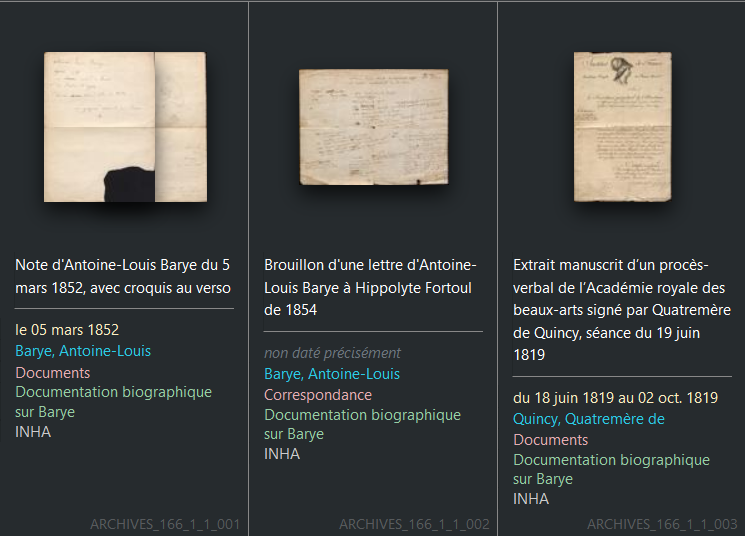
\includegraphics[width=0.8\textwidth]{barye_design_a_plat} 
        \caption{Visualisation « à plat » des documents.} 
        \label{fig:visualisation-plat} 
\end{figure}

La première forme, dite à plat, présente les pages des documents numérisés de manière juxtaposée, permettant ainsi une vue d'ensemble du corpus\footnote{Disponible à l’adresse suivante : https://barye.inha.fr/corpus}. Cette approche, simple, présente l'inconvénient de ne pas rendre compte de toute la matérialité des documents (trois dimensions, volumétrie…). 

\begin{figure}[h] 
        \centering 
        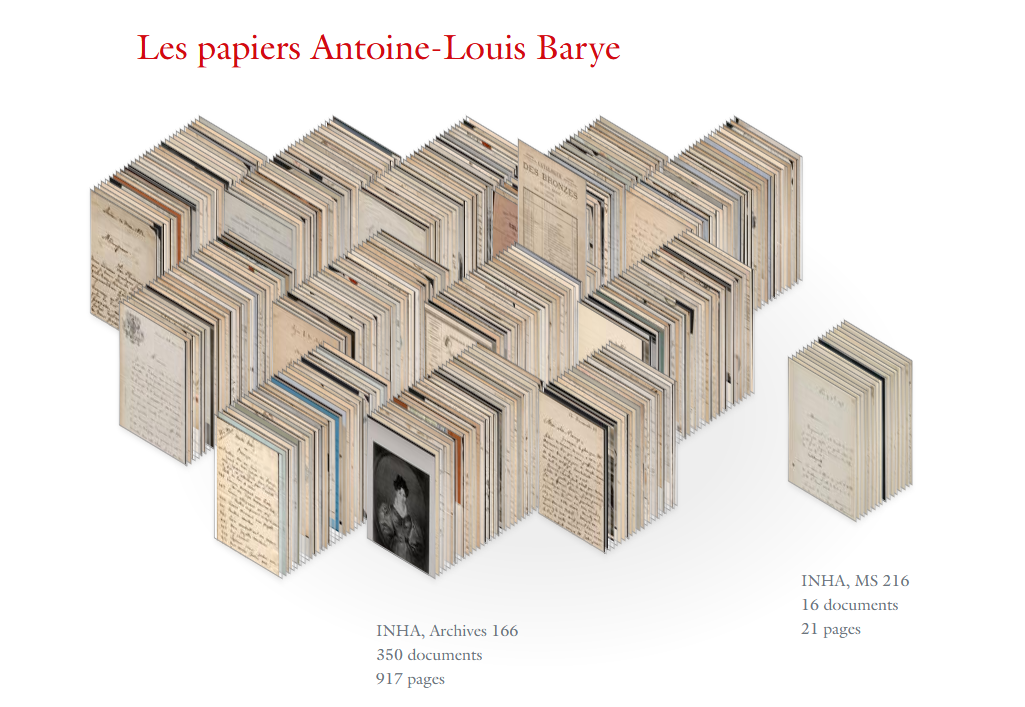
\includegraphics[width=0.8\textwidth]{barye_design_isometrique } 
        \caption{Visualisation isométrique des documents.} 
        \label{fig:visualisation-iso} 
\end{figure}

La deuxième forme, dite isométrique, vise à pallier cette lacune en offrant une représentation en trois dimensions des documents, bien que celle-ci tende à réduire la taille des documents de manière artificielle pour les rendre tous de format égal\footnote{Disponible à l’adresse suivante : https://pense.inha.fr/}. Il ne s’agit donc pas encore d’une représentation totalement réaliste.

Une troisième forme, dite de visualisation « bibliothèque » ou « étagère », qui a mis plus de deux ans à être développée, permet, elle, une représentation fidèle des proportions des documents et des volumes des corpus, offrant ainsi une expérience plus immersive\footnote{Disponible à l’adresse suivante : https://barye.inha.fr/presentation}. Le caractère massif ainsi que la relative variété (sur le plan formel) du fonds sont ici bien restituées.

\begin{figure}[h] 
        \centering 
        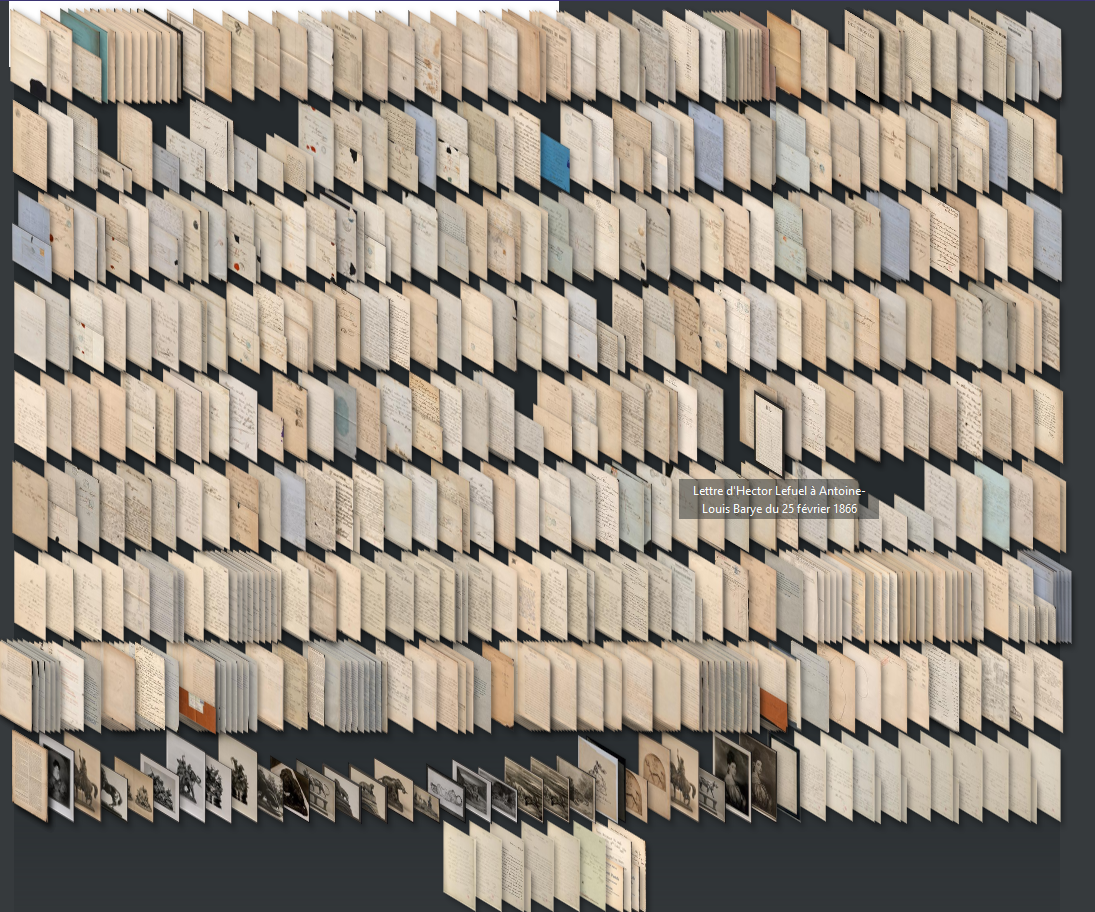
\includegraphics[width=0.8\textwidth]{barye_design_bibliotheque} 
        \caption{ Visualisation sous forme « étagère ».} 
        \label{fig:visualisation-biblio} 
\end{figure}

\begin{figure}[h] 
        \centering 
        
\includegraphics[width=0.8\textwidth]{barye_design_parcours_arts_deco} 
        \caption{Visualisation dite « en parcours ».} 
        \label{fig:visualisation-parcours} 
    \end{figure}

Enfin, la visualisation dite « des parcours », conçue comme une déclinaison de la vue bibliothèque, en mettant en valeur une sélection de documents selon des thématiques précises\footnote{Disponible à l’adresse suivante : https://barye.inha.fr/parcours/BaryeEtLesArtsDecoratifs}.


Le projet \pense accorde également une importance particulière à l’accessibilité de ses interfaces, en intégrant des standards web adaptés aux utilisateurs de lecteurs d’écran. Cette démarche, fondée sur les recommandations WAI-ARIA\footcite{initiative_wai_wai-aria_nodate} (\textit{Accessible Rich Internet Applications}), vise à structurer le code \html et JavaScript des pages pour permettre une navigation fluide et intelligible, y compris pour les personnes en situation de handicap\footcite{faulkner_using_2018}. 
Toutefois, à ce stade, le projet n’atteint que le premier niveau de ces bonnes pratiques, se concentrant principalement sur une structuration propre du \html en y ajoutant des attributs sémantiques, afin de permettre aux personnes utilisant un lecteur d’écran de saisir une partie de la richesse des pages.

\subsection{Projets d’édition numérique actuellement en cours (2024)}

\subsubsection{Des projets aux caractéristiques diverses}

\textbfit{Le projet Raoul-Rochette}\\

Le projet Raoul-Rochette, lancé en juin 2023, se concentre sur l’édition numérique d’un album de dessins d'art antique (essentiellement romain, étrusque et grec) constitué par Désiré Raoul-Rochette (1790-1854), archéologue et historien de l’art antique\footcite{gran-aymerich_raoul-rochette_2010}.
Ce projet a permis de constituer une base de données tiré de l’extraction de « composants » des dessins, segmentés selon différents critères (planches, dessins, signatures) grâce à l’utilisation de la plateforme Transkribus\footcite{inha_dessins_nodate}. Un prototype d’édition numérique a été mis en ligne, proposant une recherche à facette qui permet de filtrer les œuvres selon divers paramètres : le type de dessin, les matériaux représentés, l’aire chrono-culturelle, l’auteur du dessin, ainsi que les lieux de découverte et de production des objets représentés. Cette édition croise donc les données iconographiques en haute définition avec un commentaire érudit tiré des ouvrages de l’archéologue, favorisant une confrontation entre l'image et le texte, et s’inscrit en lien direct avec la bibliothèque numérique de l’INHA. 
Le projet est néanmoins actuellement en pause indéfinie à l'heure actuelle (2024).
\newline
\textbfit{Le projet Pressouyre}\\

Un autre projet significatif est celui consacré aux documents de fouille de l’archéologue Léon Pressouyre, assisté par son épouse Sylvia, historienne de l’art, dans la mise au jour des vestiges du cloître disparu de la collégiale Notre-Dame-en-Vaux (Châlons-en-Champagne), édifié au XIIème siècle et détruit à partir de 1759. 
Le projet, lancé en septembre 2023, porte sur l’étude des archives de Pressouyre (1935-2009), elles aussi conservées par l’\inha \footnote{Voir : https://calames.abes.fr/pub/\#details?id=FileId-3423}   qui documentent une entreprise de recherche et de reconstitution intellectuelle de plus de vingt ans. Ce fonds d’archives considérable, composé de carnets de notes, relevés et fichiers détaillant les fouilles entreprises à partir de 1963, sous la supervision de Pressouyre et de son équipe\footcite{inha_edition_nodate-1} est particulièrement remarquable, comme le souligne Isabelle Périchaud, coordinatrice du projet, de par le soin particulier qui a été apporté à l’inventaire rigoureux de chaque découverte, ce qui confère à ce fonds une richesse « exceptionnelle » \footcite{perichaud_a_2022}. 
Le projet, soutenu à nouveau par l’utilisation de Transkribus pour la transcription et la segmentation des fiches de fouille, vise également une modélisation en trois dimensions du cloître, à partir des fragments retrouvés. Cette approche plutôt novatrice (mais non complètement nouvelle pour \pense !) contribue à révéler un peu plus l’ambition expérimentale du projet. 
\newline
\textbfit{Le projet Thierry}\\

Un troisième projet notable est le projet Thierry, lancé en septembre 2023 et mené en collaboration avec Jérôme Delatour, responsable des collections photographiques de l'\inha, ainsi que les chercheuses Sipana Tchakerian et Nayiri Tcharkhoutian. Ce projet porte sur le fonds d'archives de Jean-Michel et Nicole Thierry, historiens de l'art (tous deux initialement de formation médicale),  spécialisés dans l'art arménien (auteurs avec Patrick Donabédian de l’ouvrage de référence publié chez Mazenod, \textit{Les arts arméniens}, 1987) \footcite{mouradian_jean-michel_nodate}, et vise à éditer et valoriser les nombreux documents rassemblés au cours de leurs voyages de recherche sur une période s’étendant sur 46 ans\footcite{inha_fonds_nodate}. 
Les archives, essentiellement des fiches de voyage, incluent des itinéraires, des commentaires et des photographies. Le travail de transcription (manuelle) et de segmentation (automatique) est en cours. Si la segmentation automatique a pu être mise en place du fait d’une certaine régularité de mise en forme notamment en ce qui concerne les fiches d’itinéraires, il est à noter qu’une transcription automatique par \ocr, a été écartée, et ce, bien que les documents soient tous quasi-intégralement typographiés, du fait de l’introduction de caractères non latins, comme des caractères de l’alphabet arménien, ainsi que d’un riche système d’abréviations complexes, qui nécessiteraient un entraînement spécifique du modèle d’\ocr pour produire des résultats satisfaisants. Le projet comporte une composante de visualisation cartographique des différents trajets effectués par les Thierry, avec une projection des itinéraires sur une carte, qui a fait l’objet d’un prototype mis en ligne\footcite{inha_fonds_nodate}. 
Pour chaque voyage documenté par les fiches, le trajet est projeté sur un fonds de carte pour l’instant vierge – un choix privilégié dans un premier temps, tant du point de vue technique (lisibilité des informations), que du point de vue scientifique (complexité de représentation de l’évolution des frontières au cours du temps et tensions politiques à prendre en compte émergeant de la dénomination choisie pour les lieux, notamment en ce qui concerne les territoires disputés encore aujourd’hui entre l’Arménie et l’Azerbaïdjan par exemple (citons le conflit au Haut-Karabakh)).
Enfin, il convient de souligner que l’un des aspects centraux de \pense réside dans la multimodalité de ses projets. Du traitement iconographique (\textit{Karbowsky}, \textit{Raoul-Rochette}) à la modélisation 3D (\textit{Karbowsky}, \textit{Pressouyre}), en passant par la cartographie interactive (\textit{Thierry}), \pense met en avant une approche fluide et hybride qui articule des disciplines et des méthodes variées.

\subsubsection{La correspondance Doucet/René-Jean, un statut à part ?}

\textbfit{La BAA et la Bibliothèque de l’INHA : un héritage institutionnel riche}\\

Le projet d’édition de la correspondance entre Jacques Doucet, couturier, collectionneur et mécène que nous avons déjà présenté, et René-Jean, proche collaborateur de Doucet, critique d’art et bibliothécaire de la Bibliothèque d’Art et d’Archéologie, s’inscrit dans le cadre du programme intitulé « La Bibliothèque d'art et d'archéologie de Jacques Doucet : corpus, savoirs et réseaux » \footcite{lequipe_du_carnet_edition_2021} lancé en 2018\footcite{noauthor_a_nodate}, peu après le déménagement de la Bibliothèque de l’\inha dans la salle Labrouste, en 2016\footcite[p.17-19]{cugy_histoire_2020}. Le projet s’appuie également sur la base de données « Acteurs de la BAA », disponible sur la plateforme AGORHA\footcite{inha_lettres_nodate}. 
Le programme, initié par Marie-Anne Sarda, est une poursuite d’un précédent programme mené de 2011 à 2016 sur les collections personnelles de Jacques Doucet, et coordonné par Chantal Georgel. Ce programme entend valoriser l’héritage institutionnel de Doucet, à travers la numérisation et l’étude de ses archives, conservées à la \bnf et à l’\inha. Le fonds principal sur lequel repose ce projet est le « NAF 13124 », constitué de la correspondance de Doucet et René-Jean, donnée à la \bnf en 1946 par René-Jean lui-même\footcite{inha_lettres_nodate}. Ce fonds constitue la majeure partie de l’ensemble documentaire faisant l’objet de l’édition numérique (89 sur les 98 documents recensés). Un fonds secondaire, « Autographes 143-145 », est conservé à la bibliothèque de l'\inha dans le fonds Doucet et est issu d’un don plus récent réalisé par la fille de René-Jean, Sylvie Maignan en 2006\footcite{flejou_jacques_2015}.

Le projet d’édition numérique de la correspondance au sein du projet \pense a débuté lui au printemps 2021 sous la direction de Pascale Cugy, historienne de l’art et spécialiste de la \baa\footcite[p.2]{cugy_histoire_2020}, parallèlement au développement du projet \textit{Karbowsky}, lui aussi en lien direct avec la figure de Doucet, nous l’avons dit. Il s’agissait pareillement de « confirmer » la réplicabilité des processus utilisés pour le fonds Barye. 

Il est tentant de considérer le projet d’édition de l’échange épistolaire de Doucet avec René-Jean, qui de par sa nature, sa temporalité et ses correspondants, aborde beaucoup la question de l’élaboration de la \baa ; comme ayant une place particulière au sein de l’institution. En effet, il existe un lien de filiation clair entre la \baa et la Bibliothèque de l’\inha, régulièrement volontiers présentée comme une « héritière » de la bibliothèque de Doucet. Rappelons que la \baa, constituée à partir de 1908 dans « 6 appartements de la rue Spontini » \footcite{flejou_jacques_2015}, toute entière consacrée à l’histoire de l’art et à l’archéologie, et constituée avec une approche voulue comme scientifique (intégrant des publications savantes, des archives, des fonds photographiques et iconographiques comme des dessins ou des estampes) a été donnée par Doucet à l’Université de Paris en 1917 puis rattachée à l’\inha en 2003. Par ailleurs, le fonds issu de la \baa de Doucet constitue encore une grande partie des collections de la bibliothèque de l’actuel \inha, comme le souligne Pascale Cugy\footcite[p.2]{cugy_histoire_2020}. 
La correspondance entre Jacques Doucet et René-Jean, qui nous permet d’explorer la manière dont Doucet entretenait ses relations avec ses collaborateurs artistiques et savants, apparait comme auxiliaire précieux pour comprendre la genèse et le fonctionnement de la \baa : il est donc tout naturel de la voir devenir objet d’une édition numérique à part entière dans le cadre de \pense. 
\newline
\textbfit{Les figures de Jacques Doucet et de René-Jean : brèves présentations biographiques}\\

Né en 1853, Jacques Doucet a d'abord bâti sa fortune dans la haute couture, reprenant le magasin familial situé rue de la Paix à Paris et le faisant connaître mondialement en y cultivant une clientèle prestigieuse. Collectionneur, amateur d’art, il s’intéresse d’abord aux collections XVIIIème (l’un des objets de l’édition \textit{Karbowsky}), avant de se tourner vers le mécénat d’artistes contemporains, notamment après la vente en 1912 de sa collection XVIIIème à la suite d’un traumatisme personnel, la mort brutale de sa maîtresse Jeanne Ruaud. Saisissant l’intérêt esthétique de l’avant-garde, il acquiert en 1924 les \textit{Demoiselles d’Avignon} de Picasso. Son très fort intérêt pour l’histoire de l’art, perceptible dans toutes ses entreprises (y compris ses choix artistiques en tant que couturier), prend forme avec la constitution d’une bibliothèque qui deviendra la \baa. Ses collections parvenues à la Bibliothèque de l’\inha en 2003 sont aujourd’hui conservées sous le fonds « Bibliothèque de l’INHA – collection Jacques Doucet ». Il disparaît le 30 octobre 1929 à l’âge de 76 ans.

René-Jean, de son nom de naissance René Hippolyte Jean (1879-1951), lui, est issu d’un milieu plus modeste. Il officie d’abord comme journaliste et critique d’art dès 1900, avant de devenir sous-bibliothécaire à la Bibliothèque des Arts décoratifs (1904). Il est finalement engagé le 1er septembre 1908 par Doucet en qualité de bibliothécaire, « plus comme collaborateur que comme fonctionnaire »\footnote{Extrait de la lettre d’engagement de Doucet à René-Jean : « […] Le plus sérieux est que vous devez à la bibliothèque que je forme tout votre dévouement et toute votre intelligence, que je considère prendre en votre personne plus un collaborateur qu’un fonctionnaire. », dans \footcite[p.139]{chapon_cetait_2006}}, avec pour mission de constituer une bibliothèque spécialisée dans l’histoire de l’art\footcite{sarda_rene-jean_2021}, la même qui deviendra plus tard la \baa. 

            
        \sautdepage

        %% Chapitre 2%%
        \hypertarget{chap2}{%
        \chapter{De la transcription à l’enrichissement des sources : le traitement des corpus textuels}\label{chap2-traitement-textuel}}

            Intéressons-nous à présent aux phases de traitement de la donnée textuelle, en nous penchant sur la mécanique concrète suivie par le projet \pense. Les sources historiques qui font l’objet des éditions numériques, qu’elles soient conservées par l’\inha ou par ses partenaires le sont généralement sous forme de fonds d’archives, qui doivent donc préalablement être numérisées et transformées par ce biais en format image : il s’agit de les rendre tant lisible sur écran (et ainsi valorisable auprès du public) que traitable par la machine. Au cours de la phase de numérisation, il s’agit de transformer l’objet encore matériel en « données » . Cette transformation « manufacturée » s’accompagne de processus, de traitements qui font l’objet de choix, de réflexions, d’orientation (une médiation soulignée par Johanna Drucker\footcite[p.8]{drucker_is_2013}). 
Après l’étape de la numérisation, viennent les phases d’extraction du texte à partir des images puis d’encodage du texte. Ce sont ces étapes que nous explorerons dans \hyperlink{chap3}{le prochain chapitre}. Nous nous concentrerons ici sur la chaîne de traitement appliquée en vue de l’édition du corpus de correspondance Doucet/René-Jean.

\subsection{De la numérisation à la « mise en données » : la transcription et le balisage, premières étapes de la curation de données}

\subsubsection{Politique de transcription suivie}

\textbfit{Un usage relativement hétérodoxe et assumé de l’outil Transkribus}

Pour traiter les documents manuscrits (entre autres) dans le cadre du projet \pense, l’outil Transkribus a été privilégié. Ce logiciel, développé par l’université d’Innsbruck dans le cadre du projet européen READ (\textit{Recognition and Enrichment of Archival Documents}), constitue une plateforme dédiée à la transcription de textes manuscrits. Proposant un modèle ouvert et participatif, il rassemble une vaste communauté de chercheurs, archivistes, et utilisateurs bénévoles\footcite{carius_plateforme_2020}. Le projet READ, qui a permis de créer cet outil, visait justement à établir une collaboration entre plusieurs domaines de spécialité : des archivistes, des chercheurs en sciences humaines, des informaticiens et des bénévoles\footcite{noauthor_recognition_2015}. Il permet non seulement une transcription manuelle ou automatique (au choix), mais aussi l’entraînement de modèles sur mesure, la recherche dans les transcriptions, un proto-balisage compatible avec la \tei,  l’annotation des documents et l'export dans divers formats. 

Le choix de \pense s’est porté sur Transkribus pour plusieurs raisons. Comme l'explique Sébastien Biay, Transkribus dispose d’un atout majeur en termes d’ergonomie en comparaison avec d’autres outils disponibles, notamment E-Scriptorium, dont l’utilisation s’avère plus complexe et moins aisée à appréhender par des équipes non formées techniquement\footcite[p.24]{biay_chaine_2022}. Son application en ligne (elle-même plus facile d’accès que le client expert bureau en local – comme le note également Jean-Christophe Carius\footcite{carius_plateforme_2020}, ce qui a donné lieu à l’élaboration d’une fiche explicative synthétique pour aider les chercheurs à naviguer dans le modèle de données appliqué par la logique de Transkribus\footcite{inha_schema_nodate}) demeure plus intuitive et plus facile à prendre en main par une équipe non spécialiste d’humanités numériques.  Cette dimension d’accessibilité est un facteur décisif pour le projet \pense, qui vise à impliquer les chercheurs dans l'élaboration de l'édition numérique sans toutefois les forcer à se transformer en développeurs professionnels. Il s'agit de créer un environnement collaboratif où les historiens de l'art peuvent interagir directement avec les outils numériques, tout en restant au cœur du processus de recherche, au lieu d'être isolés des enjeux techniques. 
Signalons qu’à cet effet, des tutoriels\footcite{carius_plateforme_2020} existent en ligne pour familiariser les chercheurs avec l’usage de cet outil\footcite{perrin_tutoriel_2019}.

En ce qui concerne l’export des données, Transkribus permet une extraction en \tei, un format largement utilisé pour l’encodage de textes en humanités numériques francophones. L’utilisateur peut non seulement transcrire, mais aussi baliser le texte, un balisage qui n’est pas complètement rudimentaire (possibilité d’ajouts d’attributs). Avec Transkribus, ce processus est facilité par une interface graphique intuitive, bien plus accessible pour un non-spécialiste qu’une arborescence \xml. Ainsi, les chercheurs peuvent directement baliser des éléments comme des noms de personnes (\textit{persName}), des lieux (\textit{placeName}), ou encore des événements. Un système de balisage, appuyé sur le standard \tei, en cohérence avec le public visé par le service, est proposé, mais une personnalisation demeure possible. Ce balisage s’adapte au contexte des documents étudiés, tout en permettant une personnalisation selon les besoins du projet\footcite{noauthor_pour_nodate}. 
A l’export, on obtient des fichiers \tei à l’architecture simple, en trois parties, comprenant \textbf{<teiHeader>}, \textbf{<facsimile>} et \textbf{<text>}. 

L’ergonomie de Transkribus est également saluée par d'autres projets académiques qui l’ont adopté, comme l'ANR « Foucault Fiches de lecture », où le logiciel a été utilisé pour faciliter la transcription semi-automatique des documents, grâce à une phase d'apprentissage basée sur des réseaux neuronaux (\hyperlink{chap6}{voir chapitre 6}) \footcite[p.104]{bermes_patrimoine_2020}.

Dans le domaine patrimonial, l’utilisation de Transkribus ne se limite pas aux bibliothèques et aux archives, il a aussi trouvé sa place dans les musées. Bien que le recours à la reconnaissance de texte manuscrit (\htr) reste discret dans ce milieu, comme le souligne Alix Chagué, Transkribus a joué un rôle déterminant dans son appropriation par des institutions culturelles : en effet, la quasi-totalité des musées ayant eu recours à l’\htr se sont appuyés sur le logiciel, apprécié pour permettre aux utilisateurs de maîtriser chaque étape de la chaîne de traitement, de la numérisation à l’obtention d’une extraction textuelle, et de « gérer de manière autonome leurs campagnes de transcription » \footcite[p.4]{chague_intelligence_2022}. Transkribus est apprécié en ce qu’il permet de manière ergonomique et relativement transparente pour l’utilisateur d’entraîner des modèles d’IA pour la reconnaissance optique de caractères manuscrits ou typographiés en les affinant (\textit{fine-tuning}) par des vérités terrains (\textit{ground truth}), échantillons représentatifs restreint du corpus étudié mais suffisamment important pour que le modèle puisse assimiler les motifs récurrents.
Cependant, il faut noter dans le cadre du projet \pense, cet aspect n’a pas été pleinement exploité. En effet, le projet a plutôt fait le choix de la transcription manuelle, en raison notamment de la complexité des documents traités, comme nous le verrons plus loin. 
Cette décision a été motivée par plusieurs facteurs : l’hétérogénéité des manuscrits (présence de plusieurs scripteurs pour des projets comme celui de Barye, ou mise en page irrégulière comme dans le cas de Doucet), ou encore la faible volumétrie des documents dans le cas de fonds comme celui de Doucet, insuffisante pour constituer un ensemble représentatif pour l'apprentissage d’un modèle\footcite{carius_plateforme_2020}. Si la segmentation automatique (également proposée par Transkribus) a été explorée notamment dans le cas du projet Thierry, qui semble présenter une relative régularité de mise en page, la tâche de transcription demeure manuelle, pour des raisons évoquées notamment \hyperlink{chap1}{dans le précédent chapitre} (présence de caractères non latins, abréviations non développées, ajouts manuscrits et graphies de lieux parfois non répertoriées – translittérations non fixées depuis le cyrillique ou l’alphabet arménien notamment). Nous aborderons plus en détail les raisons du choix de la transcription manuelle dans le \hyperlink{chap4}{chapitre 4}.
\newline
\textbfit{De l’importance de l’établissement d’une politique de transcription en amont}\\

Le projet d’édition numérique \pense s’est rapidement confronté à une problématique récurrente dans ce type de travail : celle de la cohérence du balisage, une difficulté qu’il aurait été possible d’éviter par une réflexion approfondie sur la transcription en amont. Comme l’indiquent Peter Robinson et Gautier Poupeau\footnote{Dans \footcite{poupeau_reflexions_2004} et \footcite{poupeau_ledition_2008}}, l’élaboration d’une politique de balisage explicite, partagée entre les chercheurs et les ingénieurs, est une étape fondamentale à mener en amont pour s’assurer de la cohérence du travail éditorial. Robinson, de son côté, insiste sur la nécessité de fonder toute édition numérique sur une politique de transcription claire et basée sur des principes explicites\footcite{blanc_feracci_quest-ce_2022}. 
Une telle anticipation aurait pu permettre de résoudre des difficultés spécifiques, notamment celle de l’application irrégulière de balises comme \textbf{`<orgName>`} et \textbf{`<work>`}, qui, dans certaines portions du corpus, sont présentes de manière inégale. Ce manque de constance dans le balisage se révèle particulièrement problématique lors du traitement automatisé des données textuelles, perturbant ainsi l’identification correcte des entités.
L’exemple du projet Thierry, où une réflexion sur le balisage est menée dès le départ, met en lumière l’importance de ce travail préparatoire, non seulement pour éviter des incohérences, mais aussi pour permettre l’intégration des exigences des chercheurs avec celles des ingénieurs. En effet, cette approche concertée favorise une meilleure harmonisation des besoins en termes de contenu scientifique et de traitement numérique, garantissant une plus grande efficacité dans la gestion des données. Cette différence d’approche entre les projets Doucet et Thierry peut en partie s’expliquer par la plus grande maturité de \pense dont bénéficie le projet Thierry, qui a débuté en 2023, à la différence du projet Doucet, qui a vu la phase de transcription et de balisage débuter bien plus tôt, à une époque où l’expérience de \pense avec Transkribus comme avec le standard \tei était peut-être moins importante.
\newline
\textbfit{Projet d’enrichissement non abouti}\\

Un projet d’enrichissement des éléments propres à la correspondance, inspiré des propositions faites dans le manuel \textit{Encoding Correspondence}\footcite{dumont_encoding_2019}, élaboré par le \tei Special Interest Group on Correspondence, et mettant en avant une série de balises TEI spécifiques adaptées à la structure et aux conventions des échanges épistolaires occidentaux, n’a pu par exemple être mené à son terme. Parmi les objectifs initialement envisagés, il était question d’ajouter des balises jugées manquantes dans le <body>, le corps du texte, parmi lesquelles : 

\begin{itemize}[label=\textbullet]
    \item \textbf{<pb/>} (\textit{page beginning}), accompagné de l’attribut @type ayant en valeur ‘folio’ : ceci afin de baliser le marquage de l’information typographique présente sur certaines lettres (dans le sous-ensemble NAF13124), dont l’origine n’est pas pleinement connue, mais qui permet de constituer, dans une approche « génétique » du fonds, un premier marqueur de la logique de classement appliquée soit par René-Jean, soit par la BnF qui a reçu la majeure partie du fonds en 1946.  

    \begin{figure}[h] 
        \centering 
        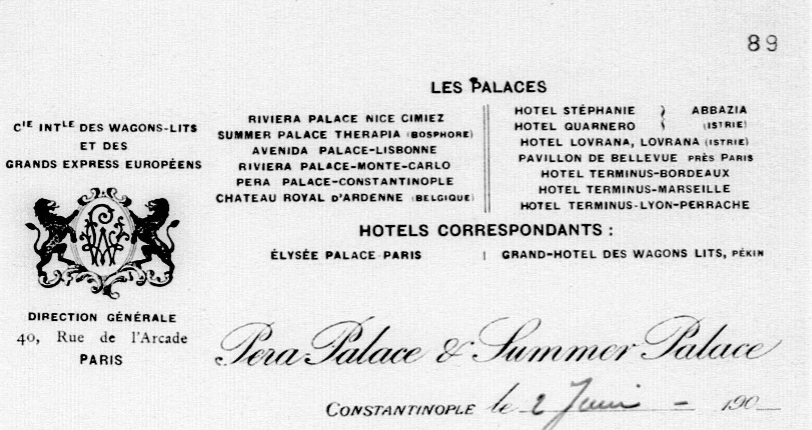
\includegraphics[width=0.8\textwidth]{folio_doucet} 
        \caption{Copie de la lettre bnf\_naf13124\_2\_62, portant la mention typographiée du « folio », « 89 » dans l’angle supérieur droit.} 
        \label{fig:doucet-folio} 
    \end{figure}

    Un autre élément de type « foliotation » manuscrit celui-là et qui n’est ni de la main de Jacques Doucet ni de la main de René-Jean, est présent dans le corpus (sous-ensemble « Autographe 143-145 ») et pourrait faire l’objet d’un balisage similaire (avec quelques variations notamment dans la valeur de l’attribut, qui serait à déterminer auprès de la responsable scientifique). Il s’agit d’une numérotation a priori indépendante de la foliotation, vraisemblablement rajoutée lors de l’archivage du corpus, possiblement par Sylvie Maignan, la fille de René-Jean, qui a effectué elle-même un classement et une numérotation des feuillets du corpus avant d’en faire don à la Bibliothèque de l’\inha au début des années 2000. 

    \begin{figure}[h] 
        \centering 
        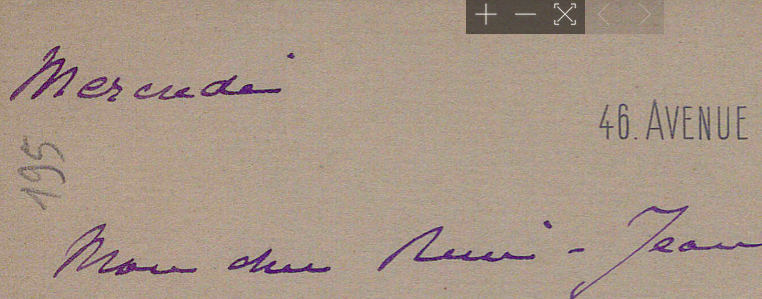
\includegraphics[width=0.8\textwidth]{numerotation_maignan} 
        \caption{Copie de la lettre BINHA, Aut. 143\_02\_195, portant la mention manuscrite de la numérotation appliquée par Sylvie Maignan, « 195 » au crayon à papier, perpendiculaire par rapport au sens de l’écriture, flanc gauche.} 
        \label{fig:doucet-maignan} 
    \end{figure}

    Lors de la transcription manuelle de la correspondance, le choix a été de marquer l’existence de ces ajouts directement dans le corps du texte, en s’inscrivant ainsi dans des choix de transcription propres à l’édition traditionnelle : l’italique et l’usage de parenthèses ont ainsi été privilégiées. Ce choix, pertinent dans le cadre d’une édition papier ou traditionnelle, n’intégrant pas l’usage d’un format balisé, peut être limitant dans le cas d’une édition \tei, en ce qu’il confond sémantique et typographie. 
    En \tei, l’information peut être rendue par le choix de balises appropriées, qui, dans un deuxième temps, lors de la phase de transformation vers l’\html, peut se traduire par des variations typographiques. L’intégration d’informations « périphériques » au texte d’origine directement dans le corps du texte peut en effet apparaître gênante lors du traitement automatique, d’où cette initiale orientation vers le choix de balise \textbf{<pb/>}, recommandée par le manuel \textit{Encoding Correspondence}. 
    \item L’usage de la balise \textbf{<add/>} comprenant l’attribut @hand et la valeur ‘RJ’ (pour René-Jean), aurait également pu permettre de baliser les passages de texte ajoutés postérieurement par René-Jean et ainsi éviter, de façon analogue au cas cité ci-dessus, l’ajout par l’éditeur du texte brut « (de la main de René-Jean) » en italique. 
    \item \textbf{<back/>} pour les informations textuelles propre à l’agencement des cartes postales (description de la carte postale située au dos de la zone de texte).
    \item \textbf{<fw/>} (\textit{form work}) accompagné de l’attribut @type et de la valeur ‘header’ pour les en-têtes de papiers à en-têtes, comme les documents portant le nom et l’adresse de l’hôtel où séjourne Doucet par exemple – cas fréquemment rencontré dans le corpus.
    \item \textbf{<stamp/>} ou \textbf{<figure @type=’cachet’/>} pour l’encodage des informations relatives aux éléments textuels rattachés à des timbres ou des tampons.
    \item L’usage de balises telles que \textbf{<signed/>} pour la signature, \textbf{<salute/>} pour la formule de politesse ou encore \textbf{<dateline/>} pour les informations de datation aurait également pu être pertinent. 
\end{itemize}

L’irrégularité de placement , vis-à-vis de ces balises, des parties textuelles qui auraient pu faire l’objet d’un balisage tel que décrit plus haut, combiné à la grande variation de ce type d’information, complique encore un peu plus leur identification et leur repérage. 
Une balise de description spécifique aux échange épistolaires dans le \textbf{<teiHeader/>} était également envisageable, il s’agit de la balise \textbf{<correspDesc/>} incluse dans le \textbf{<profileDesc/>}\footcite{tei_consortium_tei_2024}, permettant d’encoder précisément les informations relatives à chaque acteur de la correspondance, pour chaque lettre échangée.

Plusieurs obstacles ont entravé la mise en œuvre de ces enrichissements. 
D’une part, l’export \tei de la transcription manuelle obtenu via l’outil Transkribus a généré un grand nombre de balises auto-fermantes, telles que \textbf{`<lb/>`}, \textbf{`<ab/>`}, \textbf{`<pb/>`}, ou \textbf{`<fw/>`}, utilisées pour signaler la correspondance entre le texte et l’image ou pour marquer les éléments de mise en page, qui ont pu gêner la circulation dans l’arborescence \xml. Ces balises, bien qu’utiles pour la structuration visuelle du texte, se sont parfois avérées problématiques du point de vue de la préservation de la logique sémantique du balisage textuel. 
En particulier, la balise \textbf{`<lb/>`}, indiquant le passage à la ligne (\textit{line beginning}), a provoqué des coupures gênantes dans certaines balises, comme les noms de personnes. Par exemple, un nom complet écrit sur deux lignes se retrouve scindé en deux balises `<persName>`, compliquant ainsi le traitement automatique de ces données nominatives. Cet effet est exacerbé lorsque les parties textuelles concernées ne sont pas homogènes ou apparaissent de manière irrégulière, rendant plus complexe leur balisage et leur repérage ultérieur. En effet, dans une situation telle que « Jacques » apparaît en fin de ligne et « Doucet » en début de ligne suivante, le résultat suivant est susceptible de se produire : 
\begin{minted}[linenos,frame=lines,fontsize=\small]{xml}
    <persName>Jacques</persName>
    <lb/>
    <persName>Doucet</persName>
\end{minted}, provoquant, lors de l’indexation automatique, l’identification de deux entités nommées pour une seule personne. 

Les balises encapsulées, comme \textbf{`<persName>`} dans un \textbf{`<choice>`}, constituent une autre source de complications. Dans certains cas, ces balises n’ont pas été correctement identifiées par les outils de repérage utilisés, comme en témoigne l’exemple du nom « Holleau » dans le fichier bnf\_naf13124\_2\_60, où la balise \textbf{`<sic>`} (portant la valeur de l’adverbe « sic », signalant une graphie (ici de nom propre), jugée irrégulière), englobant le nom pose un problème pour certains outils de repérage des balises, du fait d’espaces surnuméraires induits par la présence d’autres balises au sein de la balise \textbf{<persName>} :
    \begin{minted}[linenos,frame=lines,fontsize=\small]{xml} 
    <persName>
        <comment>
            <choice>
                <corr/>
                <sic>Holleau</sic>
            </choice>
        </comment>
    </persName>
    \end{minted}.
\newline
\textbfit{Un héritage parfois problématique de l’édition traditionnelle}

Les difficultés rencontrées dans le projet \pense trouvent également leurs racines dans un héritage parfois pesant ou inadapté de l’édition traditionnelle, où les conventions typographiques priment souvent sur les potentialités offertes par l’édition numérique. En effet, dans certaines parties du corpus, le choix a été fait de suivre les conventions de l’édition papier, introduisant des mentions comme « (de la main de René-Jean) » directement dans le texte, en italique et entre parenthèses. Cette décision, motivée par la volonté de rester fidèle aux conventions éditoriales classiques\footcite{nougaret_ledition_2015}, a cependant posé problème dans le cadre de l’édition numérique, comme nous l’avons brièvement évoqué plus haut. 
Cette approche peut ainsi être jugée comme ne prenant pas toujours en compte les spécificités de l’édition numérique et notamment les potentialités du balisage, en confondant mise en forme finale et traitement intermédiaire du corpus : là où il serait possible d’utiliser une balise \tei sémantiquement appropriée et qui serait éventuellement restituée par une traduction typographique  respectant les conventions de l’édition classique (italique, parenthèses, mention complémentaire…), le choix a été fait d’intégrer directement dans le texte du corpus une indication éditoriale, brouillant potentiellement les lignes entre texte original et texte édité, une situation susceptible de poser problème dans le cas d’une édition qui se veut « diplomatique ».

En effet, la volonté affirmée de proposer une double lecture, à la fois diplomatique (imitative) et critique (proposant un apparat critique et une révision du texte) au lecteur\footnote{« Tout le sens du projet \pense est donc de restituer cette épaisseur du texte manuscrit, tout en donnant accès à une version éditorialisée que l’internaute pourra à loisir citer et commenter à son tour », dans \footcite[p.2]{carius_principes_2024}}, vient ainsi se heurter aux potentialités du numérique, car on peut voir dans ces complexités de balisage un mélange entre plusieurs formes éditoriales, notamment dans l’exemple de la note « de la main de RJ » : le fait d’inclure dans le texte cette mention de l’éditeur, distinguée du corps du texte par un simple marquage typographique comme des crochets ou des parenthèses, est à mettre en lien avec un réflexe éditorial critique traditionnel, et vient gêner l’édition diplomatique au sens strict (dans lequel elle n’a pas lieu d’être). 
Il est peut-être également possible de voir dans la préférence pour un balisage typographique (tel qu’avec la balise de mise en forme \textbf{<hi/>}) au détriment du balisage sémantique (\textbf{<add @hand/>}) une certaine hâte à produire une version finale du texte, sans avoir pleinement exploré les potentialités de la réflexion numérique. 

\subsubsection{Choix de balisage des textes}
\newline
\textbfit{Le standard TEI}\\

Le projet \tei se présente comme une entreprise « durable et influente » dans le domaine des humanités numériques. Conçu à la fin des années 1980 autour de l’élaboration d’une « grammaire » du langage \sgml puis \xml adaptée à l’encodage de documents patrimoniaux, il affiche pour ambition d’offrir un cadre clair, adaptable et facilement implémentable pour normaliser et  structurer la production de données textuelles, essentiellement destinées à la recherche en \shs. Comme le souligne Lou Burnard, l’un des fondateurs de l’initiative, la \tei émet des recommandations pour la création de textes numériques, en portant l’ambition de cultiver la collaboration au sein d’une vaste communauté scientifique (appuyée sur son Consortium, rassemblement d’organisations partenaires pour la plupart issues du monde universitaire)\footcite{burnard_quest-ce_2015}. 
Ces recommandations mettent particulièrement l'accent sur l'analyse sémantique du texte et garantissent une interopérabilité avec différents environnements logiciels permettant la réutilisation des données, car elles se veulent indépendantes de tout cadre technique spécifique. Le standard a connu plusieurs évolutions depuis sa première version en 1987, et la cinquième édition (P5), publiée en 2007, étant désormais fondée exclusivement sur \xml, abandonnant ainsi le \sgml utilisé dans les premières versions.
La flexibilité de la \tei permet des personnalisations étendues grâce au principe de l’\odd, qui autorise la création de schémas d’encodage adaptés à des projets spécifiques\footcite{noauthor_odd_nodate}.

Les recommandations proposées par la \tei sont compilées dans un document unique appelé \textit{Guidelines}, décrivant en détail (sous la forme de l’ODD originelle de la version P5) les bonnes pratiques pour l’encodage des textes numériques. 

Un document encodé en \tei est structuré en plusieurs sections essentielles. La première balise croisée dans l’arborescence \xml d’un texte encodé en \tei est le \textbf{`<teiHeader/>`}, qui contient l’ensemble des métadonnées du fichier (titre, nom de l’auteur, contexte de production, etc.). Cette balise se compose généralement de quatre sections principales, dont une seule est obligatoire\footcite{tei_consortium_tei_2023} : le \textbf{`<fileDesc/>`}, qui décrit les aspects bibliographiques du document électronique. Parmi les trois autres sections généralement retrouvées, citons la balise \textbf{`<encodingDesc/>`} qui documente « la relation entre le texte numérique et ses sources », à savoir, le plus souvent, la politique d’encodage adoptée ; le \textbf{`<profileDesc/>`} qui fournit des informations sur les « aspects non bibliographiques » du texte ; enfin, le \textbf{`<revisionDesc/>`} résume l’historique des modifications apportées au fichier depuis sa création, à la manière d’un fichier \textit{log}. 

La structure des documents \tei se prolonge avec la balise \textbf{`<text/>`}, qui renferme la transcription du texte divisé en plusieurs sections : \textbf{`<front/>`} pour les éléments préliminaires comme la page de titre, \textbf{`<body/>`} pour le corps principal du texte, et \textbf{`<back/>`} pour les éléments post-liminaires. 
Dans le cadre des documents générés via Transkribus par exemple, une autre balise est systématiquement introduite avant le \textbf{<text/>} : \textbf{`<facsimile/>`}, qui assure un lien entre les fac-similés des documents numérisés et leur transcription en identifiant (grâce à des balises et attributs enfants) par des points « géographiques » l’emplacement du texte (obtenu grâce à la transcription, manuelle ou automatique) au sein de l’image. 

L’usage du standard \tei n’est pas restreint à la seule recherche universitaire, bien que celle-ci demeure son domaine de prédilection. Selon des données recueillies dans le \textit{Digital Catalogue of Digital Editions}, 196 des 337 éditions répertoriées utilisent \xml-\tei comme format d’encodage\footcite{ucl_centre_for_digital_humanities_digital_nodate}. 
Cependant, il existe des cas où des projets préfèrent ne pas utiliser la \tei, comme le souligne Patrick Sahle. Deux raisons principales entrent en jeu pour expliquer ce choix : 
\begin{itemize}
    \item d’une part, l’apprentissage de la \tei peut être perçu comme chronophage, et certains projets estiment ne pas avoir les ressources nécessaires pour maîtriser ces compétences en temps limité, 
    \item d’autre part, des balises \xml personnalisées peuvent mieux correspondre aux spécificités des textes sources que celles proposées par la \tei, offrant une flexibilité supplémentaire\footcite[p.174-75]{sahle_what_2016}.
\end{itemize}
De plus, il est à remarquer que l’encodage en \tei, pour des raisons de compatibilité de caractères, est davantage adapté pour les langues à alphabet latin comme le français, l’anglais ou le latin, tandis que les langues disposant d’un alphabet non-latin ou d’un système d’écriture différent, tels que le cyrillique, l’abjad arabe ou les sinogrammes, rencontrent encore des difficultés d’implémentation dans ce format\footcite[p.177]{sahle_what_2016}.

En France, l’utilisation de la \tei (assez largement partagé dans les projets d’éditions numériques), est plutôt encouragé dans le cadre des projets soutenus par des grandes institutions de recherche. Comme le note \citeauthor{chateau-dutier_editions_2021}, le \textit{Guide des bonnes pratiques numériques} de 2009, rédigé par le Très Grand Équipement Adonis, devenu Huma-Num, recommande explicitement le recours à cette norme pour l’encodage de documents dans le cadre de projets de recherche en \shs\footcite{tge-adonis_guide_2009}. Château-Dutier remarque par ailleurs que l’adoption de la \tei par le milieu de la recherche française, demeure relativement récent : le premier projet français à avoir utilisé la \tei ayant été l’édition des cours d’Antoine Desgodets en 2008\footcite[p.81]{chateau-dutier_editions_2021}. Aujourd’hui, la \tei est devenue un standard largement adopté pour les éditions critiques numériques dans la sphère des humanités numériques francophones\footcite{blanc_feracci_quest-ce_2022}, et notamment en histoire de l’art\footcite[p.82]{chateau-dutier_editions_2021}.
\newline
\textbfit{Les libertés prises par le projet \pense vis-à-vis du standard TEI}\\

Le projet \pense, bien qu’aligné sur le standard \tei, a pris certaines libertés vis-à-vis des recommandations officielles. Il est important ici d’introduire les notions de « conformité » et de « validité » : si, dans le contexte étudié dans ce chapitre, la \textbf{conformité} (ou le caractère « bien formé » d’un document) se réfère au respect de la syntaxe \xml (garanti par exemple par la présence d’une déclaration \xml avant la racine du document, par le respect du principe de non-chevauchement des balises et de l’architecture arborescente propre à \xml, par exemple) ; la \textbf{validité}, elle, concerne le respect de la grammaire particulière, ou du schéma, appliqué au \xml – ici, il s’agit du respect de la « grammaire » \tei : à savoir, le respect de la logique de balisage introduite par \tei : certaines balises ne peuvent être enfants d’autres balises par exemple. Un document conforme peut donc être invalide. 
Le caractère invalide d’un document peut entraîner des problèmes d’interopérabilité, notamment lorsqu’il s’agit d’appliquer des traitements automatiques sur le fichier, nécessitant ainsi un pré-traitement supplémentaire. 

Un exemple concret des choix inhabituels réalisés par le projet \pense concerne l’utilisation d’identifiants non uniques (@xml:id). En effet, l’attribut @xml:id, ayant pour rôle de donner un identifiant unique à des entités déterminées (comme des noms de personnes avec <persName/> ou des noms de lieux, avec <placeName/> par exemple), ne peut avoir qu’une valeur unique dans tout le document encodé\footcite{marsh_xmlid_2005}. Or, lors de la mise en place de l’édition Doucet-René-Jean et de la mise en place de l’identification, cette règle n’a pas été complètement respectée.  Une solution possible pour corriger cette situation est d’intégrer un index des personnes dans la balise \textbf{`<profileDesc>`}, définissant ainsi chaque identifiant unique une fois pour chaque document et permettant de référencer ces identifiants dans le \textbf{`<body>`} du document à l’aide de l’attribut @ref accompagnée d’une valeur identique à la valeur de @xml:id mais précédée d’un croisillon (« # »). 
Bien que cette méthode permette de se conformer tant aux \textit{Guidelines} \tei qu’aux bonnes pratiques d’encodage \xml, sa mise en œuvre est susceptible de s’avérer chronophage. 
L’autre alternative, déjà pratiquée par \pense dans le cadre de l’édition \textit{Barye}, consiste à ne pas utiliser l’attribut @xml:id, mais de lui préférer l’attribut @ref accompagné d’une spécification quant au référentiel utilisé pour formuler l’identifiant (comme @ref-agorha, @ref-idref ou @ref-wikidata). 

Par ailleurs, la question de l’utilisation d’une \odd dans le cadre de \pense mérite d’être posée. L’ODD permet de créer un schéma de validation personnalisé pour une édition numérique au format \tei. Comme le souligne \citeauthor{biay_chaine_2022}, certains projets nécessitent un degré de précision et de spécificité tel qu’il devient nécessaire de produire une ODD\footcite[p.72]{biay_chaine_2022}, mais cela ne semble pas être le cas pour le projet \pense. Étant donné la diversité de nature des projets d’édition numérique, la création d’une \odd n’apparaît pas comme une priorité pour \pense, même si cette option pourrait être envisagée si l’encodage devait devenir plus complexe à l’avenir.

\subsection{L’encodage des métadonnées : transformations appliquées aux en-têtes TEI}

\subsubsection{Enrichissement des métadonnées}

Les transformations appliquées aux fichiers \tei du projet \pense ont permis d’enrichir les métadonnées. Pour réaliser ces modifications, des technologies telles que XQuery et XPath, correspondant aux spécifications du \wwwc, ont été utilisées. Ces langages sont particulièrement adaptés à la manipulation de données en \xml-\tei, car ils permettent de naviguer efficacement dans l’arborescence des fichiers, en passant aisément d’un élément parent à ses éléments enfants. Comme le rappelle Anderson, XQuery est compact, concis et relativement facile à apprendre, ce qui en fait a priori un outil de choix pour les humanistes numériques\footcite{anderson_teaching_nodate}. 
Langage installé sur le Web depuis plus de vingt ans, sa longévité constitue également paradoxalement sa limite fondamentale, en ce que la documentation disponible tend à être ancienne et rattachée à des environnements obsolètes (bien que le langage lui-même n’ait pas grandement évolué depuis la publication de la documentation).  En plus de faciliter les transformations, l’interface de BaseX, utilisée dans le projet, permet de réinjecter directement les modifications dans la base de données.
XQuery s’est révélé particulièrement utile pour l’ajout d’informations manquantes aux fichiers \tei générés par Transkribus, pour la normalisation des données, ainsi que pour l’insertion d’identifiants pérennes à certains éléments.

Le choix des ajouts à opérer pour l’encodage des métadonnées s’est inspiré d’autres projets ayant utilisé la \tei comme le \textit{Thomas Gray Archive}, dont la structure \tei choisie propose une présentation relativement riche des métadonnées\footnote{Voir par exemple le fichier suivant : https://www.thomasgray.org/texts/poems/txt_GrayTh1716_wdeho.xml}.

Les fichiers sur lesquels nous avons travaillé étant directement issus de l’export \tei produit à partir de la transcription Transkribus, l’encodage du \textbf{<teiHeader/>} était particulièrement rudimentaire, ne comprenant que le titre (pour lequel la convention de nommage lors de la transcription avait privilégié l’indication de la cote avant la présentation du contenu), la date lorsqu’elle avait été précisée par l’opérateur effectuant la transcription, ainsi que le nom de l’institution porteuse du projet, la cote, la typologie documentaire, le nombre de page et la langue. 
Nous avons donc choisi d’effectuer les ajouts et transformations suivants, grâce à un script XSLT encapsulé dans un script XQuery  :

\begin{itemize}[label=\textbullet]
    \item \textbf{<projectDesc/>} et \textbf{<editorialDesc/>} à partir de l’exemple proposé par \textit{The Thomas Gray Archive}
    \item normalisation et suppression des cotes dans les titres
    \item ajout d’un identifiant pérenne (IDREF ou AGORHA) pour les noms d’auteurs, grâce à un attribut @ref
    \item ajout d’un identifiant pérenne \ark de la \bnf dans le \textbf{<seriesStmt/>} pour les documents issus du fonds conservé à la BnF
    \item indication du nom de la responsable scientifique du projet dans le \textbf{<respStmt/>}
    \item normalisation des URL (suppression des espaces et des virgules, susceptibles de gêner le traitement automatique du corpus). 
\end{itemize}[label=\textbullet]

\subsubsection{Préparation en amont d’une fonctionnalité d’interface}

La chercheuse en charge du volet scientifique du projet, Marie-Anne Sarda, a émis le souhait d’une interface finale qui puisse permettre de naviguer aisément entre les différentes collections de la \baa de Jacques Doucet. 
Ce désir s'appuyait sur une typologie d'objets d'art mentionnés dans la correspondance de Doucet, parmi les objets classifiés à l'aide de la balise \textbf{`<work>`}. La fonctionnalité  devrait reposer sur une présentation visuelle de type « cartes \textit{Bootstrap} » des œuvres mentionnées, chaque carte représentant une catégorie d'objets collectionnés par Doucet, comme les estampes, imprimés, photographies ou encore les dessins. En cliquant sur ces cartes, les utilisateurs pourraient accéder à des informations plus détaillées sur les œuvres concernées citées dans la correspondance et, idéalement, les admirer, grâce à de potentiels partenariats avec des institutions de conservation. Cette démarche s'inscrit dans un effort de visualisation visant à permettre aux lecteurs de comprendre concrètement les œuvres dont il est question dans la correspondance de Doucet. Notre travail s’est donc concentré sur la manière d’établir la meilleure façon de préparer en amont, grâce à l’encodage \tei, la future exploitation de cette typologie d’œuvres par les fonctionnalités d’interface. Il s’agissait d’identifier, pour chaque typologie isolée par la chercheuse, les lettres mentionnant des œuvres correspondant à cette typologie, pour permettre à terme leur recherche par facettes.

Pour parvenir à cet objectif, un processus en quatre étapes a été suivi : 
\begin{itemize}
    \item La première a consisté en la création par la chercheuse d'un fichier Excel contenant un alignement entre les lettres individuelles et les typologies d'objets d'art évoqués dans ces lettres.
    \item Ensuite, ce fichier Excel a été transformé en fichier \csv, choisi pour des questions d’interopérabilité, alignant plus clairement les identifiants des lettres avec ceux des typologies.
    \item Dans un troisième temps, un script Python a été utilisé pour modifier les identifiants et les faire coïncider avec ceux présents dans la base de données, en ajoutant une nouvelle colonne dans le \csv.
    \item Enfin, un script XQuery a été employé pour traiter les données du \csv, les transformer en fichier \xml, et enrichir la base de données \tei avec les informations contenues dans ce fichier.
\end{itemize}
   
\subsection{L’encodage du corps du texte}

\subsubsection{Protocole suivi pour l’enrichissement des noms de personnes}

Les noms de personnes, identifiés pour la plupart par la balise \textbf{<persName/>} ne présentaient, à quelques exceptions près (telle que l’usage de la balise @key pour certaines occurrences du nom de Doucet) aucune forme d’enrichissement lors de la reprise des fichiers obtenus par export \tei de la transcription effectuée sur le Transkribus. Il s’agissait donc de permettre une indexation optimale pour les noms de personnes.  

Le processus a débuté à nouveau avec la création d'un fichier Excel de travail par la chercheuse, contenant la forme normalisée (« Nom, Prénom ») du nom des personnes, une courte note biographique, ainsi que leur lieu d'exercice. Ce fichier avait vocation à devenir la source de valeurs pour l’ensemble des attributs choisis pour l’enrichissement : 
\begin{itemize}[label=--]
    \item l’attribut @key présente un format et une graphie normalisée des noms de personnes (« Nom, Prénom »)
    \item l’attribut @xml:id comporte une valeur d’identifiant unique, composée par la première lettre du prénom concaténée au nom de famille entier. Ce choix, apparemment arbitraire, a été cependant motivé par un souci d’intelligibilité du code – il aurait été tout à fait envisageable de choisir un identifiant unique de type \uuid, qui aurait néanmoins souffert d’une certaine opacité. Par ailleurs, la volumétrie de la base traitée étant limitée, la choix d’un tel identifiant n’a pas semblé indispensable.
    \item l’attribut @type indique l’occupation, la profession ou la relation par rapport à Doucet, sur la base des informations fournies par la chercheuse.
    \item l’attribut @subtype désigne ici le lieu d’exercice ou de résidence rattaché à la personne. Cette utilisation diffère légèrement des recommandations \tei\footcite{tei_consortium_tei_nodate}, en ce qu’il ne s’agit pas d’une information d’importance moindre que l’information indiquée dans l’attribut @type, mais d’une donnée indépendante.
    \item l’attribut @ref-agorha fournit quant à lui, lorsque disponible, un lien \ark vers la notice AGORHA de la personne concernée. 
\end{itemize}

Le processus d'enrichissement s'est déroulé en neuf étapes :
\begin{itemize}
    \item La première a consisté en une simplification manuelle du fichier de personnes fourni par la chercheuse.
    \item Un fichier \csv a ensuite été créé pour contenir les variations graphiques des noms de personnes trouvées dans le corpus de correspondances. Pour chaque nom, plusieurs versions graphiques étaient alors alignées (la variation trouvée dans le corpus, la version corrigée et la version dite « unifiée » (sous le format devant être intégré à l’attribut @key)).
    \item Un script Python a alors permis de fusionner les données du fichier d'origine simplifié avec celles du \csv produit précédemment, aboutissant à la création d'un nouveau fichier \csv.
    \item Après quelques modifications manuelles supplémentaires, un autre script Python a réorganisé ce fichier par ordre alphabétique et y a ajouté un numéro d'ordre.
    \item Enfin, un script XQuery a permis de transformer ce \csv en fichier \xml, enrichissant la base de données \tei avec les informations nouvellement obtenues.   
\end{itemize}

            
        \sautdepage

        %% Chapitre 3 %%
        \hypertarget{chap3}{%
        \chapter{Visualisation des données de la recherche : enjeux de représentation et d’intelligibilité}\label{chap3-dataviz}}

            \subsection{« Parler aux yeux » (Playfair) : de l’intérêt et des limites de la visualisation}\footnote{Expression empruntée au statisticien William Playfair, dans Eléments de statistique, Paris, 1802, cité dans \footcite{courtin_rapport_2019}}

Le Service numérique de la recherche de l’\inha, bien avant la mise en place du projet \pense, a développé ou commandité des projets de visualisation de données dans le cadre de la valorisation et de l’accompagnement de la recherche menée au sein de l’Institut. Citons parmi ces projets la visualisation sous forme de réseau réalisée dans le cadre du programme de recherche « Répertoire des acteurs du marché de l’art en France sous l’occupation » (RAMA)\footcite{inha_repertoire_nodate}, ou encore les cartographies interactives des données de la base RETIF (« Répertoire des tableaux italiens dans les collections publiques françaises ») \footcite{inha_repertoire_nodate-1}. 
Dans le cadre de \pense, la visualisation des données semble envisagée dès que les données s’y prêtent, soit en adoptant une approche « traditionnelle » de la datavisualisation, en empruntant des formes de modélisation bien établies (la cartographie avec le projet Thierry), soit en explorant des voies connexes, ancrées plutôt dans le design graphique, exploitant la matérialité du corpus pour en offrir une visualisation permettant d’en saisir l’aspect massif (\textit{Barye}) ou d’en restituer l’ambition ou la genèse intellectuelle (\textit{Karbowsky}). Pour toutes ces approches, diverses dans leurs objets et leurs héritages conceptuels, le \snr revendique ouvertement une démarche de  \textit{data storytelling}\footcite{inha_visualisation_nodate}, un concept qu’il peut a priori paraître étonnant de voir émerger dans le domaine des \shs, mais dont l’histoire est pourtant bien entrecroisée avec ces disciplines, notamment dans leur dimension quantitative.

\subsubsection{Recherche d’intelligibilité par la construction narrative : le data storytelling et son application par le SNR}

Le \textit{data storytelling}, ou narration de données, est un concept issu partiellement du monde de l’entreprise (avec notamment la notion voisine de \textit{business intelligence}) et du journalisme\footcite{sanders_developing_nodate}. La promesse du \textit{data storytelling} est de rendre intelligible des informations complexes à travers des représentations visuelles. Ce procédé est particulièrement pertinent dans un contexte où les chiffres et les analyses quantitatives sont souvent présentés de manière abstraite, rendant la compréhension difficile pour les non-initiés. La visualisation de données permet ainsi d’atténuer certains biais liés à une présentation exclusivement numérique des résultats, bien que certains inconvénients inhérents à cette approche méritent d’être discutés, notamment dans le domaine de la recherche scientifique. Nous y reviendrons plus tard.

Le \textit{data storytelling} peut être défini comme l’art de transformer des données brutes en une narration cohérente, rendant ainsi les informations non seulement compréhensibles, mais également exploitables. Comme le souligne \citeauthor{shao_data_2024}, cette pratique consiste à « tisser des faits, des insights, des émotions et des intentions dans une narration engageante qui imbue de sens des idées complexes » \footcite{shao_data_2024}. L’objectif est d’impliquer le public, de le pousser à réfléchir, voire à agir. En appliquant cette définition au domaine de la visualisation de données, le \textit{data storytelling} permet de donner vie aux données, les rendant accessibles et compréhensibles par un large public, tout en facilitant la prise de décision basée sur ces informations (d’où le lien avec la \textit{business intelligence} mentionnée plus haut).
\newline
\textbfit{Regard historique sur la visualisation de données}\\

Bien que le concept de \textit{data storytelling} apparaisse (et soit régulièrement marketé) comme une innovation récente, il s’inscrit dans une tradition plus ancienne de la visualisation des données. Dès les XVIIIème et XIXe siècles, les premiers praticiens de la statistique et de l’analyse de données ont compris l’importance de la présentation visuelle pour rendre intelligibles des questions complexes à un public non spécialisé. Kosara et MacKinlay (cités par  \citeauthor{shao_data_2024}) notent que ces premières tentatives de visualisation ressemblaient déjà aux pratiques actuelles du \textit{data storytelling}, leur objectif étant de montrer, d’expliquer ou de souligner l’ampleur de certains problèmes à des décideurs ou à des publics peu familiers des chiffres. La présentation visuelle ne doit pas se contenter de montrer des chiffres ; elle doit également donner du sens à ces chiffres et permettre de dégager des tendances claires et exploitables. Cette approche a profondément influencé le développement de la visualisation des données, tant dans le domaine scientifique que dans le domaine commercial\footcite{shao_data_2024}.

Le \textit{data storytelling} s’inscrit ainsi dans une histoire plus large de la visualisation des données, elle-même étroitement liée aux évolutions épistémologiques de la statistique. Lev Manovich, dans son analyse de l’histoire de la discipline, identifie trois phases marquantes\footcite[p.19-20]{manovich_data_2015}. 
La première phase, qui s’étend du XVIIIe siècle jusqu’à la première partie du XIXe siècle, est marquée par la collecte et la tabulation de données sociales et économiques. Durant cette période, des pionniers comme William Playfair développent des techniques graphiques de nos jours désormais incontournables, telles que le diagramme en barres, le graphique en courbes, le diagramme circulaire et le graphique en secteurs. Ces premières tentatives ne permettaient cependant de visualiser qu’une seule dimension des objets étudiés, limitant ainsi la portée analytique des représentations.
La deuxième phase, entre les années 1830 et 1890, voit l’apparition de techniques « analytiques et graphiques » permettant d’étudier les relations entre les phénomènes. L’introduction des concepts de corrélation et de régression à la fin du XIXème engendre l’utilisation du diagramme de dispersion, ou \textit{scatterplot}, pour représenter graphiquement ces relations. Cette étape marque une avancée significative dans l’utilisation de la statistique pour visualiser les liens entre différents ensembles de données.
Enfin, la troisième phase, s’étendant de 1900 à 1930, est caractérisée par la systématisation et l’extension des concepts statistiques, notamment grâce aux travaux de Karl Pearson, Charles Spearman, Ronald Fisher et Charles Pierce. Ces chercheurs ont raffiné les concepts tels que la moyenne et la médiane, et ont mis au point des méthodes pour analyser les relations entre deux variables. Cette phase marque la fondation de la statistique moderne, avec des outils et des concepts qui perdurent aujourd’hui dans les domaines de l’analyse quantitative et de la visualisation de données\footcite[p.19-20]{manovich_data_2015}. 

L’histoire de la visualisation de données est aussi marquée par son application dans le domaine de la santé publique, notamment pour représenter la propagation des épidémies. À partir du XVIIIe siècle, avec l’émergence des statistiques modernes, la visualisation devient un outil majeur pour comprendre les dynamiques des populations et de la santé et ainsi envisager de les prévenir et de les anticiper. John Snow au milieu du XIXème siècle, par exemple, utilisa une superposition cartographique pour retracer les sources de l’épidémie de choléra à Londres (et ainsi tenter de l’enrayer), tandis que Florence Nightingale employa des diagrammes en rose pour illustrer les causes de la surmortalité des soldats de la Guerre de Crimée (et ainsi proposer des méthodes hygiéniques pour y remédier). Enfin, le \textit{diagramme de Sankey} de Charles Joseph Minard, retraçant l’émiettement de l’armée napoléonienne lors de la Retraite de Russie, est aujourd’hui considéré comme l’une des visualisations de données les plus emblématiques « de tous les temps », comme le remarque Elyse Graham\footcite[p.450]{graham_introduction_2017}.
Ces premiers « récits de données » visaient non seulement à illustrer l’ampleur de certaines crises sanitaires, mais également à sensibiliser voire à pousser les autorités à agir, comme l’ont relevé, entre autres\footnote{Voir à ce sujet le rôle de la visualisation cartographique dans la prise de conscience des inégalités liées à l’accès des populations non-blanches à l’eau potable dans un quartier du Midwest des Etats-Unis : \footcite{jeffries_how_2014}}, \citeauthor{shao_data_2024}.
\newline
\textbfit{Datavisualisation et SHS}\\

La visualisation de données, dont l’intégration dans les \shs n’est pas récente, ne relève pas toujours tout à fait du réflexe dans le domaine des humanités traditionnelles, en partie en raison du fait qu’elle est souvent (voire exclusivement, pour un certain nombre de représentations canoniques) associée au traitement de données quantitatives. Selon \citeauthor{pawlicka_data_2017}, la forte poussée vers l’intégration systématique des techniques de visualisation de données dans ces disciplines peut même être interprétée comme une tentative de « scientification » des humanités, visant à défendre leur financement en les rapprochant des sciences dures\footcite[p.526]{pawlicka_data_2017}, qui disposeraient, elles, du point de vue d’un certain côté de la société et l’échiquier politique, d’une forme de légitimité à s’établir comme « véritables sciences ». Selon plusieurs auteurs, la démarche adoptée par la datavisualisation, lorsqu’implantée systématiquement, cherche à présenter des résultats empiriques dans un format qui, bien que visuellement convaincant, ne correspond pas toujours à la nature des recherches en sciences humaines, où la complexité et la multiplicité des interprétations doivent être prises en compte. Comme nous le verrons plus loin, la datavisualisation constitue bien une médiation, une interprétation de l’information à part entière, et non une simple représentation factuelle.  

Cependant, en dépit de ces critiques relatives aux biais inhérents à la représentation interprétée de la donnée et à une dimension quantitative qui a pu historiquement inspirée de la méfiance dans le domaine des humanités traditionnelle, il est légitime de constater que la force du data storytelling et de la data visualisation en général réside avant tout dans sa capacité à rendre les données plus intelligibles et plus attractives pour un large public, permettant ainsi de capter l’attention du récepteur. Une visualisation bien conçue peut ainsi rendre explicite une information souvent noyée dans des discours scientifiques difficiles d’accès\footcite{shao_data_2024}.
\newline
\textbfit{Rendre intelligible l’information complexe}\\

La relation entre la visualisation et la cognition humaine n’est pas nouvelle. Plusieurs auteurs\footnote{Parmi lesquels \footcite[p.451]{graham_introduction_2017} et \footcite[p.536]{pawlicka_data_2017}} mettent en avant une donnée anatomique qui expliquerait le succès de la visualisation de données : près de « 30\% du cortex humain est dédié au traitement des informations visuelles », expliquant le rôle donné à la visualisation de la transmission et l’acquisition de la connaissance.    Son efficacité réside dans leur capacité à transformer des données abstraites en récits visuels engageants, en introduisant une véritable « médiation » \footcite[p.80-99]{hinrichs_defense_2019} (au sens proche de celui de vulgarisation), facilitant ainsi la compréhension et la prise de décision.
\newline
\textbfit{Choix de datavisualisation dans le cadre du projet PENSE}\\

Dans le cadre du projet \pense, plusieurs choix de datavisualisation ont été faits pour illustrer et rendre accessible l’édition numérique des lettres échangées entre Jacques Doucet et son bibliothécaire René-Jean. Ces choix sont justifiés par la volonté de mettre en avant les différents événements de la vie de Doucet, de ses collections et des relations épistolaires qu’il entretenait, tout en fournissant un accès direct aux lettres et aux informations pertinentes.

Le premier outil développé est une chronologie interactive\footcite{noauthor_chronologie_nodate}, qui propose une visualisation permettant une mise en évidence de son processus de constitution de collections (achats, ventes, etc.), alignée sur des données biographiques.

\begin{figure}[h] 
\centering 
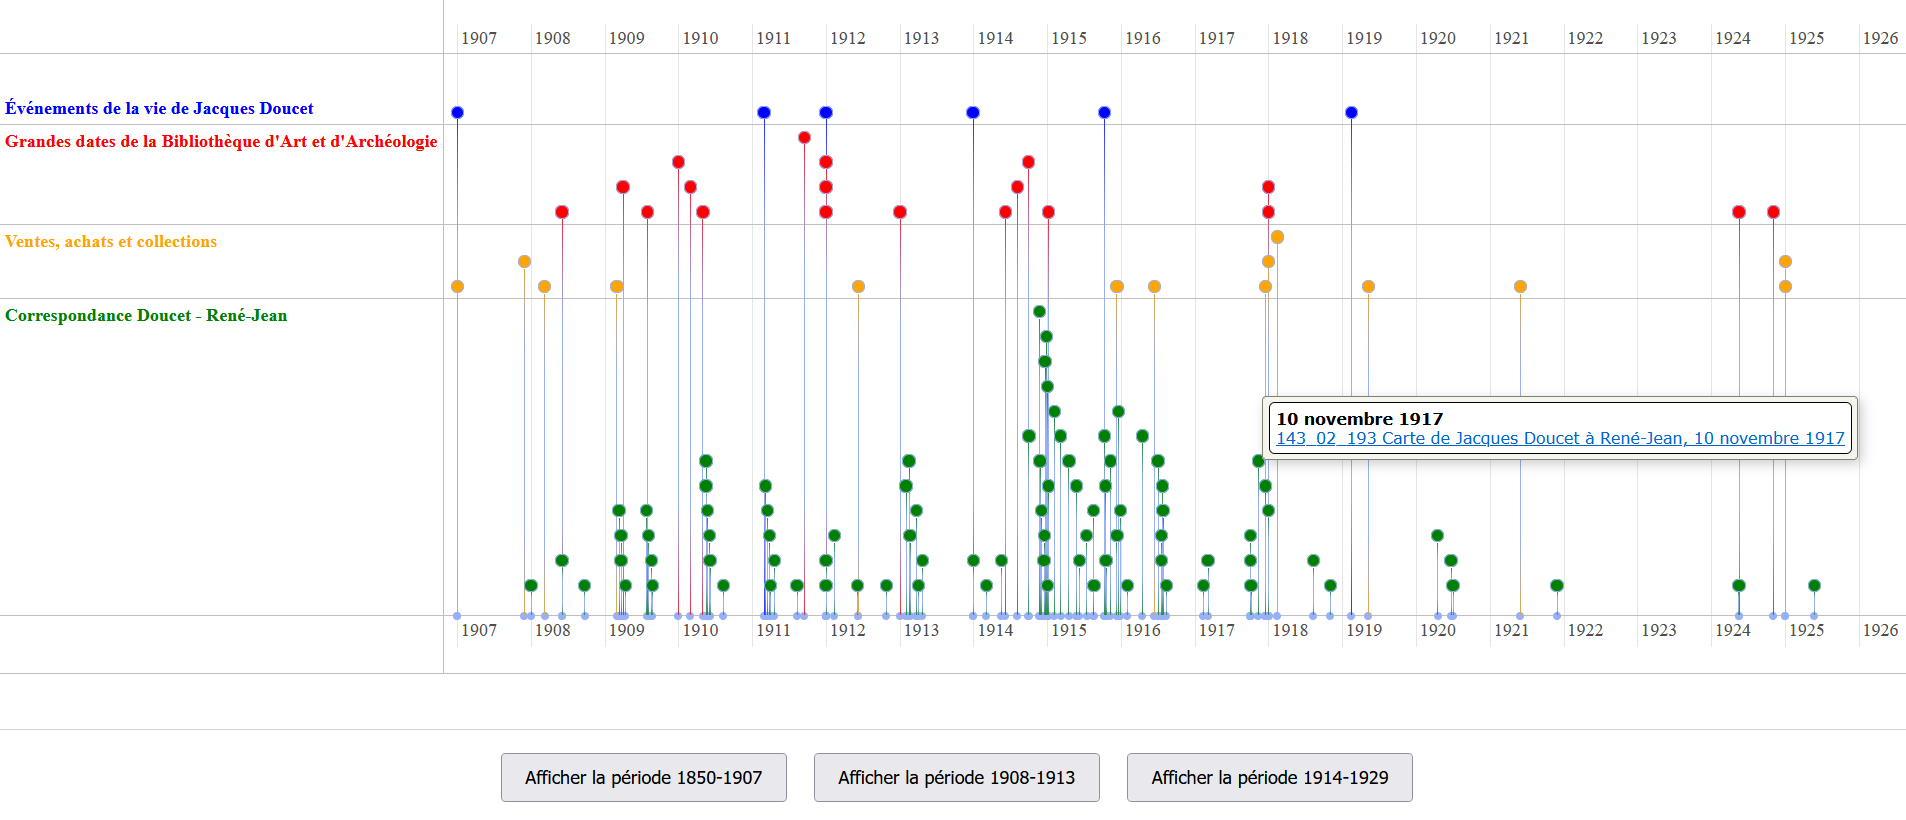
\includegraphics[width=0.8\textwidth]{chronologie} 
\caption{Prototype de chronologie interactive réalisée dans le cadre du stage pour le projet d’édition Doucet/René-Jean.} 
\label{fig:prototype-chrono} 
\end{figure}

Ce dispositif permet d'aligner sur une même ligne temporelle des dates relatives à des événements importants dans la vie de Doucet, les étapes principales de l'élaboration de la \baa, ainsi que la circulation des œuvres ayant appartenu à Doucet, le tout superposé sur la correspondance entretenue avec René-Jean, qui constitue l’arrière-plan principal de la visualisation. L’intérêt principal de cette chronologie réside dans sa capacité à synthétiser des données complexes sous une forme immédiatement lisible et accessible. Chaque événement est codé par une couleur spécifique permettant de distinguer facilement les catégories (correspondance, acquisition, vente, etc.). En survolant les points de la frise, une fenêtre informative apparaît, proposant un court descriptif de l’événement, souvent accompagné d'une image jugée évocatrice afin de renforcer l’immersion et la compréhension. De plus, pour la partie dédiée à la correspondance, l’utilisateur peut accéder directement à chaque lettre d’un simple clic, facilitant ainsi la navigation et l’interaction avec les documents originaux. Ce choix de datavisualisation, au-delà de son efficacité visuelle, permet une interaction fluide et intuitive avec le corpus.

La deuxième visualisation développée dans le cadre du stage est de forme cartographique\footcite{noauthor_carte_nodate}.

\begin{figure}[h] 
\centering 
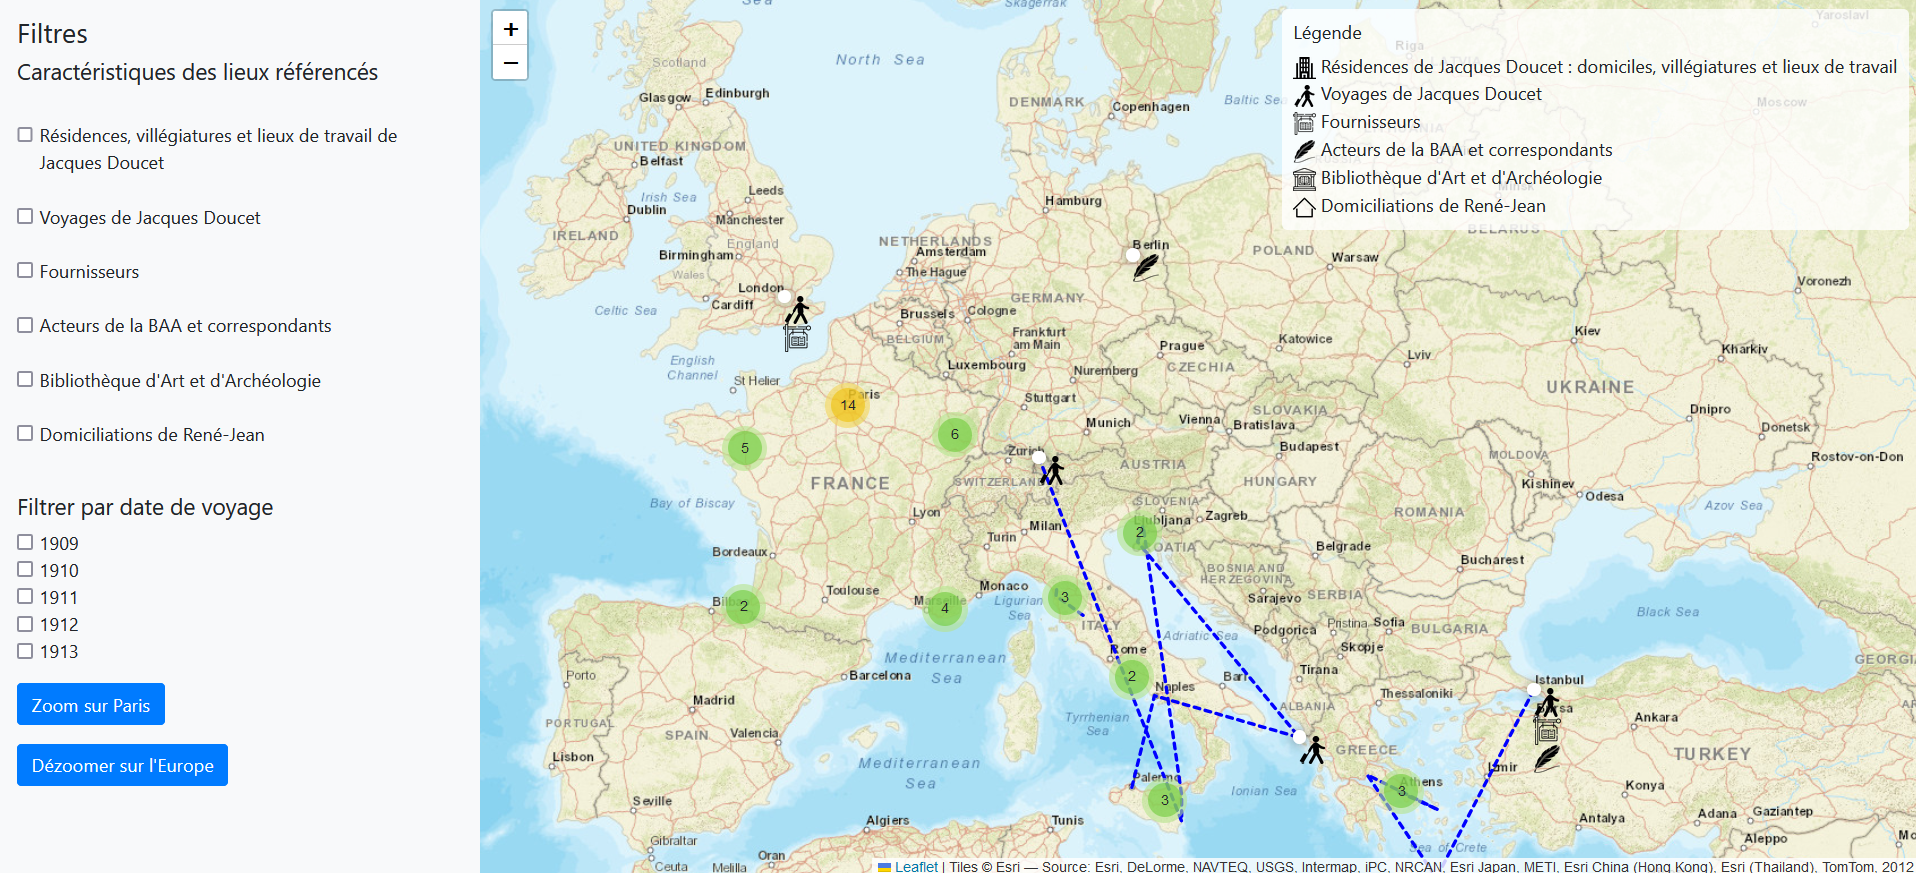
\includegraphics[width=0.8\textwidth]{cartographie} 
\caption{Prototype de cartographie interactive réalisée dans le cadre du stage pour le projet d’édition Doucet/René-Jean.} 
\label{fig:prototype-carto} 
\end{figure}

Cet outil permet de localiser géographiquement les lieux mentionnés dans la correspondance, qu’il s’agisse de résidences, d’étapes de voyages ou de localisations de fournisseurs et partenaires de Doucet. La carte est enrichie par des facettes de recherche permettant à l’utilisateur de filtrer les informations selon différents critères, tels que les résidences ou les voyages, ce qui facilite l'exploration des données spatiales du projet. 
Cette carte, en lien direct avec la correspondance, permet d’illustrer visuellement les réseaux de relations et d’échanges entretenus par Doucet à l’échelle internationale. Toutefois, elle est également soumise à des biais inhérents aux choix et contraintes technologiques et aux limites des sources. Par exemple, certains noms de personnes ou de lieux n’ont pas pu être inclus en raison de difficultés liées à l’identification ou à la qualité des sources, ce qui entraîne des lacunes dans la représentation des partenaires de Doucet sur la carte.

\subsubsection{La \textit{visual literacy} et la gestion des biais}

La datavisualisation est un outil puissant, mais elle comporte des limites importantes, notamment en ce qui concerne la manière dont elle est interprétée. La notion de \textit{visualisation literacy} (ou \textit{visual literacy}, selon les auteurs) met en lumière ces enjeux, en soulignant que même une visualisation bien conçue peut être mal comprise si le récepteur n’a pas les compétences nécessaires pour interpréter les données correctement. 
La \textit{visualisation literacy} est définie par \citeauthor{shao_data_2024} par la capacité à interpréter avec précision les représentations visuelles des données, et à extraire, traiter et tirer des conclusions à partir de celles-ci\footcite{shao_data_2024}. Cette compétence apparaît de nos jours comme une faculté critique dans une société où l’information visuelle (fondée ou non sur des données factuelles) circule abondamment, et où le recul à prendre face à ces représentations doit faire partie intégrante de l’apprentissage du citoyen\footcite[p.454]{graham_introduction_2017}.

Cependant, la responsabilité ne repose pas uniquement sur l’utilisateur, mais également sur le producteur des visualisations. C’est ici que la notion de biais entre en jeu, comme l’explique Johanna Drucker, qui propose de considérer les données non pas comme des faits objectifs existants par eux-mêmes indépendamment de tout contexte (« data »), mais comme des éléments construits et issus d’un travail d’interprétation et de reconceptualisation dans leur importation dans le milieu numérique (« capta »). Selon elle, les visualisations graphiques sont le produit d’un processus interprétatif, où chaque choix de représentation influe sur la manière dont les informations sont perçues. La distinction entre « data » et « capta », pour Drucker, renvoie à la différence fondamentale entre un savoir supposé objectif, « allant de soi », et une connaissance qui est en fait « manufacturée », construite et interprétée à partir de points de vue éminemment subjectifs\footcite[p.5]{drucker_humanities_2010}. En d’autres termes, créer une datavisualisation consiste à fabriquer du « capta » à partir de « capta », c’est-à-dire à prendre des éléments préexistants et à les organiser selon des structures qui sont elles-mêmes des « capta », conditionnées par des objectifs et des biais spécifiques. La transformation d’objets tels que le texte ou les œuvres d’art en données, phénomène voisin de celui décrit ici, est aussi critiquée chez Urzsula Pawlicka\footcite[p.531]{pawlicka_data_2017} comme comportant des risques d’effacement d’informations.
\newline
\textbfit{Quels biais à l’œuvre dans les prototypes de visualisation produits pour l’édition Doucet - René-Jean ?}\\

Dans le cadre des tâches de visualisation effectuées lors du stage, les choix de visualisation ont également été influencés par plusieurs facteurs techniques et théoriques, à commencer par les contraintes technologiques, temporelles et de compétences. 
Concernant la carte, par exemple, les outils utilisés, tels que la bibliothèque JavaScript Leaflet, ont offert des possibilités techniques importantes, notamment en termes d’ergonomie, de prise en main et d’interopérabilité (Leaflet étant la bibliothèque la plus fréquemment utilisée sur le Web pour la production de visualisations cartographiques), mais ces choix ont aussi imposé des contraintes. Le choix du fond de carte est l’un des principaux exemple de biais induit par un choix technologique, car il se base sur des représentations modernes qui ne correspondent pas toujours à la réalité historique des époques concernées. Le choix s’est porté sur un fonds de carte non vierge (contrairement à celui utilisé dans le cadre du projet Thierry par exemple) pour des raisons de compréhension, préférant invoquer à une représentation annotée (et familière) du monde, ce qui permet à l’utilisateur non spécialiste d’identifier rapidement les zones géographiques représentées. Cependant, le fonds de carte n’est pas historiquement juste, il ne correspond pas à la réalité géopolitique du monde tel que Doucet et René-Jean l’ont connu, ce qui constitue une lacune majeure.  L’idéal aurait été d’intégrer un fonds de carte correspondant à l’époque représentée, ce qui était possible techniquement en ayant recours à un fonds de carte d’atlas du début du XXème siècle libre de droit et accessible sur Gallica par exemple, combiné à un outil tel que QGIS pour la création cartographique. Cependant, en raison de contraintes tant technologiques (Leaflet étant plus facile d’accès) que temporelles, cette possibilité n’a pas été pleinement explorée. 
Par ailleurs, compte tenu des grands bouleversements géopolitiques ayant eu lieu sur la période couverte par la correspondance (1909-1928), un seul fonds de carte historique n’aurait pas constitué une visualisation complètement adéquate. On aurait pu envisager l’usage de plusieurs fonds de carte, organisés par tuilage, variant selon la période représentée, mais cela aurait soulevé des difficultés techniques et conceptuelles majeures, notamment en termes de cohérence de lisibilité des informations. 

D’autres biais ont pu émerger, et sont à signaler, dans la représentation des lieux ou des personnes. Certains noms de partenaires de Doucet, par exemple, n’ont pas pu être traités correctement en raison d’un traitement computationnel des sources qui n’a pu parvenir à saisir toutes les occurrences, notamment celles qui ne faisaient pas l’objet d’un balisage, ce qui conduit naturellement à des lacunes informationnelles dans la visualisation. 

Dans un autre domaine, les icônes utilisées dans la cartographie pour représenter certaines informations (résidences, voyages, correspondants, etc.) sont également sujettes à des biais culturels. La manière dont un lieu de villégiature ou un voyageur est représenté visuellement peut varier en fonction des conventions culturelles et graphiques, influençant ainsi la perception de ces informations. Nous nous sommes ici essentiellement basés sur une représentation occidentale contemporaine, fortement influencée par la signalétique commerciale notamment, en reprenant un style de pictogrammes que nous pourrions croiser dans notre vie quotidienne.

Dans le cas de la chronologie, il nous faut remarquer que notre visualisation a été fortement influencée par le premier prototype réalisé pour le projet par l’ingénieur en charge, réalisé à partir de la bibliothèque Vis.js, une solution technologique choisie pour sa facilité d’accès et sa rapide prise en main.

\begin{figure}[h] 
\centering 
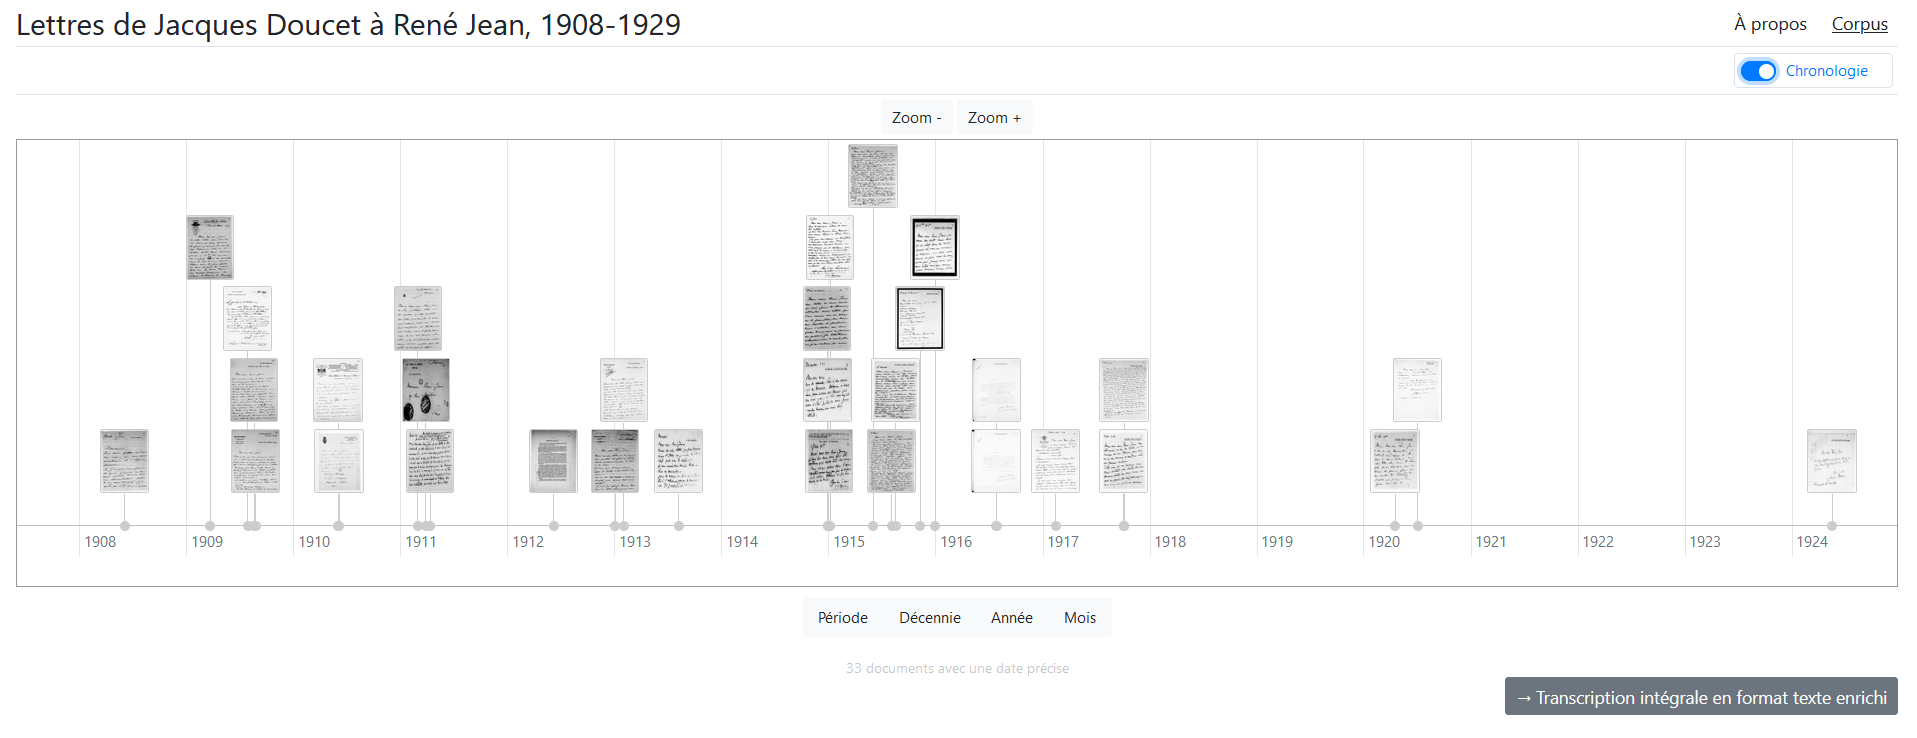
\includegraphics[width=0.8\textwidth]{prototype_prealable_chrono} 
\caption{Prototype de chronologie interactive réalisée par Jean-Christophe Carius pour le projet d’édition Doucet/René-Jean.} 
\label{fig:chrono-jcc} 
\end{figure}

Outre les aspects conditionnés par les contraintes particulière de cette solution logicielle (un « style » de visualisation relativement limité, une moins grande liberté offerte qu’avec D3.js, bibliothèque plus puissante mais moins accessible), certains biais semblent propres à la visualisation chronologique : choix des dates retenues, ce qui relève de la direction scientifique du projet, d’une part, et modélisation du temps, d’autre part (quel séquençage du temps opérer ? Un découpage par mois, par année ?). Nous avons privilégié une approche modulaire, permettant à l’utilisateur, par un système de zoom, de décider du point de focalisation de la chronologie : l’utilisateur peut ainsi techniquement zoomer jusqu’au niveau du jour individuel, les lettres étant associées à leur date précise (au jour près) de production. 

Ainsi, comme mis en évidence dans la présentation de nos choix, la datavisualisation, comme le souligne (entre autres) Johanna Drucker, n’est pas une simple représentation neutre de faits, mais le résultat d’un processus de sélection et d’interprétation où des choix et contraintes techniques et méthodologiques influencent directement le produit final.

\subsection{La datavisualisation comme partie intégrante du processus heuristique de recherche}

\subsubection{La datavisualisation comme « outil procédural » au centre de la philosophie de PENSE}

Dans la philosophie du projet \pense, la datavisualisation n’est pas seulement un outil de communication des résultats (comme elle pouvait peut-être l’être dans son acception initiale, chez Playfair par exemple), mais un véritable instrument heuristique au cœur du processus de recherche et de l’élaboration de la connaissance. Stalph et Heravi, cités par \citeauthor{sanders_developing_nodate} affirment que les datavisualisations remplissent à la fois une fonction épistémologique et une fonction communicative, il ne s’agit donc pas simplement de valoriser l’aboutissement d’une recherche, mais également de faire de la visualisation de données un nouveau point de départ pour de nouvelles analyses\footcite[p.6]{sanders_developing_nodate}, se rapprochant en cela de l’usage de la modélisation conceptuelle, permettant de poser un regard « neuf » sur les phénomènes étudiés. 
En ce sens, elles deviennent un véritable « outil procédural », intervenant dès la phase exploratoire, permettant de comprendre les données en cours de recherche, avant de les communiquer ensuite une fois les analyses terminées \footnote{\footcite[p.1645]{stalph_exploring_2021} cités par \footcite[p.6]{sanders_developing_nodate}}.     

Ce rôle central de la datavisualisation dans le processus de recherche se rapproche de la philosophie du \textit{design thinking}(\hyperlink{chap5}{voir chapitre 5}), où la modélisation visuelle est un moyen d’explorer des idées et de faire émerger de nouvelles perspectives. Dans le cadre de la mise en place des visualisations pour le projet \pense, cette démarche a été adoptée à travers un dialogue permanent entre les chercheurs et les développeurs, avec des prototypes visuels régulièrement mis à jour pour affiner les visualisations. Par exemple, les icônes et les appellations utilisées dans la cartographie ont fait l’objet de plusieurs reprises et révisions, illustrant le caractère itératif du processus. Cela souligne également l’idée que la datavisualisation n’est pas seulement une représentation finale, mais un élément central du processus d’élaboration de la connaissance.
La métaphore du château de sable, proposée par certains chercheurs\footcite{hinrichs_defense_2019}, illustre bien cette conception de la datavisualisation comme un processus dynamique et évolutif, où chaque visualisation est à la fois une « provocation esthétique » (cf. la dimension « attrayante » de la représentation visuelle de l’information), un « processus dynamique de questionnement » (cf. la dimension heuristique) et un « médiateur » pour la transmission efficace de l’information scientifique (cf. la dimension communicative). 
            
        \sautdepage

    %% PARTIE II %%
    \part{La philosophie PENSE : une approche originale au sein des projets français en humanités numériques}

        %% Chapitre 4%%
        \hypertarget{chap4}{%
        \chapter[Lutter contre un certaine « boîte noire » technologique]{Lutter contre une certaine « boîte noire » technologique : \\ \ favoriser l’implication des chercheurs dans l’établissement des projets numériques}\label{chap4-boite-noire}}

            L’un des objectifs principaux et réaffirmé des acteurs de \pense côté numérique est le décloisonnement entre ingénieurs et chercheurs : il ne s’agit pas de limiter le numérique à la réalisation isolée d’interfaces de valorisation, mais au contraire d’inviter les chercheurs à s’y intéresser et à y contribuer pleinement – sensibiliser le monde de la recherche, d’autant plus dans le domaine de l’histoire de l’art. Ce positionnement, tendant volontiers vers une discussion politique, en opposition avec l’idée selon laquelle une technologie efficace serait nécessairement une « boîte noire », c’est-à-dire un système complexe et opaque, voire hermétique dont les mécanismes demeuraient inaccessibles aux non techniciens, est au centre de la philosophie revendiquée par le projet, et en dicte plusieurs approches. 

\subsection{Une stratégie revendiquée : « approche web » contre « approche applicative »}

\subsubsection{Recherche d’accessibilité contre quête de performance}

Cette opposition entre « approche web » et « approche applicative » est comprise dans le contexte présent comme une opposition entre :  

\begin{itemize}[label=\textbullet] % premier niveau de la liste (point rond)
    \item une démarche valorisant les technologies dites du « web », à savoir des technologies (langages et formats), 
    \begin{itemize}[label=--] % deuxième niveau de la liste (tiret)
        \item permettant de structurer et d’exposer des données hébergées sur le web 
        \item accessibles par l’intermédiaire d’un navigateur,
        \item généralement installées depuis plusieurs années dans le paysage web et dont l’histoire est souvent intimement liée au développement de ce dernier 
        \item appuyées sur des standards établis et partagés, 
        \item faisant l’objet de spécifications par le World Wide Web Consortium, organisme de standardisation assurant une certaine garantie d’interopérabilité quel que soit le navigateur et le système d’exploitation utilisé pour accéder aux contenus ; 
    \end{itemize}
    \item une démarche apparaissant davantage : 
    \begin{itemize}[label=--]
            \item tournée vers l’indépendance par rapport au web et aux navigateurs, permettant de concevoir des applications tournant directement un système d’exploitation par exemple,
            \item comme une approche valorisant plutôt l’innovation et la performance et incorporant volontiers une dimension commerciale dont cherchent à s’écarter les technologies traditionnelles du web. 
    \end{itemize}
\end{itemize}

Cette opposition, dont les contours demeurent parfois flous, est particulièrement perceptible dans le discours tenu par l’équipe du projet et dans les choix technologiques réalisés. 
Ainsi, comme l’affirme Jean-Christophe Carius, si des solutions technologiques relativement récentes comme les \textit{frameworks} « tout-JavaScript » (tels que React ou Vue) – assimilé ici à une technologie « non-web », ce qui peut être discutable sur certains points, JavaScript étant généralement groupé dans la catégorie des technologies « web », y compris sous sa forme de langage de backend – sont fréquemment plébiscités dans le monde industriel en raison de leur capacité à gérer des applications à forte charge et à grande échelle (un concept que l’on désigne par le terme de « scalabilité »), il est pertinent de s'interroger sur leur choix pour des projets d’humanités numériques, qui ne partagent a priori pas les mêmes besoins, dans l’écrasante majorité des cas.  On observe parfois une attirance (peut-être par une forme de mimétisme) pour ces outils dans le monde académique, au détriment de technologies web pourtant jugées plus accessibles, plus pérennes et tout aussi efficaces pour les besoins des chercheurs en humanités. 
Cette adoption vue comme « excessive » par certains acteurs du projet, de solutions industrielles dans un contexte de recherche académique peut être questionnée : quelle est la véritable valeur ajoutée de ces outils complexes lorsque l’on travaille sur des problématiques propres aux sciences humaines et sociales ? N’y a-t-il pas pourtant un risque de perte d’intelligibilité, de trop grande complexité des outils et des contenus ainsi développés ?  Un risque d’isolation de l’ingénieur par rapport au chercheur ?
S’inscrivant en faux contre cette tendance (qui demeure cependant encore modeste dans le monde des humanités numériques francophones), \pense tend à entretenir une philosophie de relative simplicité quant à ses choix technologiques, mettant en avant l’accessibilité et la transparence et rejetant une certaine complexité perçue comme inutile. Le recours à des technologies web « simples » et ancrées depuis longtemps dans le paysage d’Internet (\html, CSS…) permet d’inclure un plus grand nombre de chercheurs, qui ont plus de chances d’y avoir été familiarisés. Cela ne signifie pas pour autant un refus complet de la technologie avancée, mais un recentrage sur des outils adaptés aux besoins spécifiques de la recherche.

Cette approche rejoint très partiellement celle du mouvement « low-code », voire « no-code », une tendance qui vise à proposer des outils accessibles sans nécessiter des compétences en programmation. Si ce mouvement suscite parfois des critiques (sécurité, accusation d’ « illettrisme numérique » \footcite[p.3]{cahier_comment_2022}, etc.), il n’en reste pas moins une voie intéressante pour l’inclusion de chercheurs non techniciens dans des projets numériques. Un exemple probant dans le domaine des humanités numériques est l’outil \textit{ImageGraph}, développé par Leonardo Impett, qui permet de manipuler des graphes d’images sans avoir à écrire de code complexe\footnote{Voir l’URL suivante : https://www.meshs.fr/page/imagegraph cité dans \footcite{aubry_artificial_2021}}, cité dans Aubrey et al. Le cas des \cms ou logiciels de gestion de contenu, dont font partie Wordpress, Drupal et Omeka est un autre exemple plus largement utilisé dans le domaine des SHS pour construire et maintenir des sites web à moindre coût.
Le mouvement no-code offre une réponse pour le moins radicale à une problématique récurrente dans le domaine des humanités numériques : celle de savoir si les chercheurs en humanités numériques doivent ou non apprendre à coder. Comme le souligne Consoli (cité par \citeauthor{anderson_teaching_nodate}), ce débat divise la communauté des humanités numériques. Certains estiment en effet qu’il est contre-productif pour les chercheurs de s’investir dans l'apprentissage du code, arguant que cela détourne leur attention de leur véritable objectif scientifique\footcite{anderson_teaching_nodate}.

\subsubsection{S’inscrire dans les principes démocratiques du Web}

Le choix de recourir à une application web plutôt qu’à une application indépendante du Web s’inscrit dans une vision qui privilégie l’ouverture et l’accessibilité. Comme le stipulent les principes éthiques du Web, « \textit{the web is for all people} », et l’utilisation du Web ne devrait pas, selon ces principes, nécessiter un niveau élevé de compétences techniques. En ce sens, les technologies web se doivent d’être « intelligibles » et « ouvertes » afin de permettre une appropriation par un large public, sans exiger des compétences en développement\footcite{noauthor_ethical_nodate}. 
Cette démarche fait aussi partiellement écho aux initiatives d’ouverture des données dans le cadre de la recherche scientifique (accessibilité, circulation de l’information). En France, ces principes sont fortement encouragés, notamment avec la promotion des principes \fair \footcite{wilkinson_fair_2016}. Ces principes, en phase de diffusion dans la communauté scientifique internationale, visent à garantir que les données produites dans le cadre de la recherche soient facilement trouvables, accessibles à tous, interopérables avec d’autres systèmes, et réutilisables par d’autres chercheurs.

Le projet \pense s’inscrit dans cette logique d’ouverture, cherchant à favoriser la circulation des connaissances à travers des technologies web accessibles. Une ambition entérinée au niveau institutionnel avec la diffusion de la \textit{Charte pour l’ouverture des données de l’Institut national d’histoire de l’art}\footcite{nurra_pratique_2023}.

Cependant, notons que cette ouverture des données n’est pas sans coût. Comme le note plusieurs auteurs, ouvrir les données implique souvent des processus longs et coûteux pour les chercheurs et les ingénieurs, notamment en termes d’anonymisation et de gestion des aspects légaux\footcite[p.60]{aubry_artificial_2021}. Ce défi est particulièrement sensible dans les sciences sociales, où il est parfois difficile de concilier ouverture et protection des données sensibles et de doser entre « suffisamment ouvert » et « suffisamment fermé » \footcite{bendjaballah_sciences_2023}, phénomène également abordé par Etienne Anheim qui souligne la surcharge de tâches non directement académiques\footnote{Anheim parle cependant ici spécifiquement de tâches administratives qui ne relèvent pas de la recherche académique à proprement parler.} dans le quotidien des chercheurs\footcite{anheim_administrer_2018}. Il faut cependant noter que cet aspect ne concerne pas directement le cadre de \pense, du fait de la relative ancienneté des sources traitées.

\subsection{Une certaine prise de distance avec les procédés d’automatisation}

\subsubsection{Préserver « le goût de l’archive » (Arlette Farge) : importance du recours aux tâches manuelles}\footnote{\textit{Le Goût de l'archive} est le titre d’un ouvrage très fréquemment commenté d’Arlette Farge (1989) traitant de la relation intime entre le chercheur en histoire et les sources primaires}

Le concept de « goût de l’archive » proposé par l’historienne Arlette Farge, dans l’ouvrage éponyme publié en 1989, souligne l’importance du lien intime entre le chercheur et l’archive dans sa matérialité, dans sa dimension physique, tangible et souvent fragile. Un lien repensé (mais non pas écarté\footcite{clavert_gout_nodate}) à l’ère du numérique avec la transformation de l’archive en « donnée », traitable non seulement plus par l’humain, mais par la machine, installant une médiation supplémentaire qui n’existait pas auparavant.
\newline
\textbfit{Transcription manuelle contre HTR : raisons scientifiques, logistiques et organisationnelles d’une préférence}\\

La transcription manuelle demeure, pour nombre de spécialistes, une activité fondamentale du travail sur les sources. Elle n’est pas simplement une étape technique de reproduction d’un texte, mais représente un véritable travail d’analyse et d’appropriation critique. Comme le font remarquer plusieurs auteurs dans des contextes différents, la transcription est déjà en elle-même une forme d’analyse scientifique, s’inscrivant pleinement dans le travail du chercheur\footcite[p.80]{dufournaud_humanites_2014}, complémentant le travail de commentaire critique (qui peut la suivre ou la précéder) et permettant une véritable « appropriation » du texte, rapprochant la source du chercheur, et dont l’encodage est la suite logique\footnote{« L’encodeur est l’accoucheur du texte » selon Frédéric Duval, dans \footcite[p.15]{duval_pour_2017}}. 
Ce processus est couramment vu auprès des chercheurs non techniciens comme une alternative plus enrichissante que la simple correction d’erreurs issues d’une sortie \ocr ou \htr (reconnaissance par la machine des caractères ou de l’écriture manuscrite), tâche considérée comme aliénante car réduisant le chercheur à un rôle de correcteur typographique, limitant l'interaction avec le contenu à une dimension mécanique et non analytique. Certains chercheurs se détournent aussi des technologies de reconnaissance optique des caractères, non seulement pour des raisons scientifiques, mais aussi parce que ces technologies ne sont pas toujours fiables ou adaptées à des corpus trop peu volumineux ou trop complexes. C’est par exemple le cas du Fonds Thierry, que nous avons déjà évoqué, où la reconnaissance de caractères a échoué en raison de la présence de graphies non latines que l’\ocr n’a pas su déchiffrer. Ce cas illustre les limites de l’automatisation, qui nécessite, même dans le meilleur des cas, une intervention humaine (correction) pour garantir une transcription fiable\footcite{chague_intelligence_2022}.

La méfiance envers l'automatisation dans la transcription se reflète également dans le rejet de ce que certains perçoivent comme une « industrialisation »\footcite[p.83]{chateau-dutier_editions_2021} du processus éditorial. Selon certaines critiques, la chaîne automatisée, qui peut s’étendre de la segmentation à la transcription en passant par le balisage, a pour effet de distancier le chercheur de la source et de transformer une activité intellectuelle en une simple procédure de production. Ce processus est perçu comme l'antithèse de l’approche attentive et critique habituellement attendue dans l’étude des archives.
D’autre part, certaines méthodes de transcription plus spécifiques, comme la transcription imitative, qui consiste à reproduire fidèlement les particularités d’un texte, y compris ses erreurs orthographiques et grammaticales, ont également suscité des débats. Cette méthode, envisagée dans le cadre du projet d'édition numérique des archives Doucet, repose sur une volonté scientifique de fidélité maximale au texte d’origine (édition diplomatique). Toutefois, même des chercheurs expérimentés, (dont des chercheurs ayant travaillé auprès de \pense et dont les propos ont été recueillis par l’intermédiaire de l’ingénieur en charge du projet) ont souligné la difficulté qu’il peut y avoir à produire manuellement un texte imitatif fidèle. En effet, il n'est pas aisé pour un scripteur formé aux normes orthographiques et syntaxiques contemporaines de respecter consciemment les fautes et variations présentes dans un texte d'époque, ce qui complique la réalisation d'une transcription véritablement « authentique » et rend la tâche peut-être plus pénible.
Par ailleurs, en dépit de l’intérêt scientifique que peut représenter la transcription humaine, d'autres solutions sont parfois envisagées pour pallier le caractère chronophage de la transcription manuelle par les chercheurs, mais ces dernières présentent elles-mêmes des limites importantes. L’externalisation vers des prestataires professionnels ou le recours à des amateurs bénévoles dans des initiatives de crowdsourcing sont des pistes souvent étudiées\footcite{chague_intelligence_2022}. Néanmoins, ces alternatives comportent également leurs propres défis, soulignés par \citeauthor{chague_intelligence_2022}, que ce soit en termes de coûts ou de contrôle qualité.
Dans le cas précis des archives Doucet, la fidélité au texte original, qui a contribué à orienter la décision vers une transcription manuelle, s’inscrit dans une perspective d’édition « diplomatique », c’est-à-dire une reproduction la plus exacte possible des documents dans leur forme d’origine\footcite{masai_principes_1950}, y compris les erreurs et anomalies\footcite{gvelesiani_quest-ce_2017}. Cette approche est jugée essentielle dans le cadre de l’édition critique, car elle permet de restituer au plus près la forme du texte avant toute intervention éditoriale\footcite[p.18]{duval_pour_2017}. Toutefois, l’édition Doucet se distingue par sa double ambition. D’une part, elle vise à produire une édition de type diplomatique, fidèle en tous points à l’orthographe (parfois fautive) et à la mise en forme d’origine, d’autre part, elle cherche à proposer une édition critique plus « traditionnelle », comprenant des corrections permettant la pleine intelligibilité du texte\footcite{carius_principes_2024}.
\newline
\textbfit{Une possible méfiance vis-à-vis de l’informatique ?}\\

Il est important de souligner que le projet \pense ne prend pas parti sur l’usage ou non des technologies d’automatisation, mais cherche avant tout à s’adapter aux besoins des chercheurs. La dimension exploratoire est présente, notamment dans les essais d’automatisation des processus de correction après une première phase de transcription imitative, nous le verrons dans \hyperlink{chap7}{le chapitre 7}, mais demeure balisée par l’objectif principal du projet, qui reste centré sur les attentes scientifiques des équipes de recherche. 
Enfin, une certaine méfiance persiste vis-à-vis de l’informatique en général. Comme le rappelle Berra, ce scepticisme repose en partie sur des « représentations sociales » ambivalentes de l’informatique. D’un côté, elle est perçue comme porteuse de progrès et de liberté, mais de l’autre, elle est aussi vue comme un vecteur de bureaucratisation et de déshumanisation\footcite[p.614]{berra_pour_2015}. 
Certaines critiques dénoncent également ce qu’elles appellent le \textit{technological hipsterism} (Earhart), c’est-à-dire une tendance à privilégier l’innovation technologique pour elle-même (« \textit{innovation for innovation’s sake} », comme le formule \citeauthor{earhart_digital_2012}), au profit d’une recherche effrénée de nouveauté et au détriment de la qualité scientifique du travail\footcite[p.24]{earhart_digital_2012}. Le projet \pense se distance clairement et explicitement de cette approche, privilégiant la rigueur scientifique sur l’innovation pour l’innovation. 

\subsubsection{Frilosités institutionnelles possibles vis-à-vis de l’intelligence artificielle}

Le recours à l’\ia dans le domaine de l’automatisation des processus de transcription ou d’analyse textuelle soulève des questions à la fois techniques et politiques. À une époque où l’IA générative semble accessible à tous, il paraît naturel de vouloir intégrer ces technologies dans le champ de la recherche. Cependant, cette intégration soulève des préoccupations, notamment en ce qui concerne la souveraineté des données et des outils utilisés, et plus largement la dépendance possiblement induite à des entreprises privées étrangères pour l’accès à des jeux de données ou à des outils.
\newline
\textbfit{Enjeux politiques : souveraineté des données et du code}\\

L’un des premiers aspects à relever concerne la compréhension du réel fonctionnement des outils d’IA disponibles pour la recherche (crainte d’une « boîte noire ») et la question de l’ouverture des données, une dimension plutôt essentielle pour la mise en place de protocoles de recherche, comprenant une réflexion sur la réplicabilité des expériences, par exemple. L’une des distinctions à effectuer lorsque l’on parle de transparence dans le domaine de l’IA concerne la différence entre l’ «\textit{open source} », qui désigne une transparence totale du code, et les « \textit{open weights} », qui n’ouvrent qu’une partie des paramètres d’entraînement d’un modèle d’IA (typiquement un grand modèle de langage) sans en rendre public le code complet\footcite{ramlochan_openness_2023}. Un certain nombre de \llm à l’heure actuelle relèvent de l’open source, comme les modèles LLAMA de Meta, Mistral de Mistral AI ou BERT de Google, tandis que d’autres demeurent propriétaires, comme GPT d’OpenAI. 
Si ces approches apportent une très relative transparence, elles ne freinent pas les craintes quant aux questions de souveraineté, qui se posent, notamment pour des applications dans des domaines stratégiques\footcite[p.77]{pollotec_intelligence_2018}. Les applications dans le monde de la culture, qui ne relève pas à proprement parler d’un secteur « stratégique » au sens où l’entend traditionnellement le monde politique (qui voit plutôt dans cette appellation des domaines régaliens comme la défense ou le maintien de l’ordre public), sont tout de même soumises à des enjeux de souveraineté proche, notamment en ce qui concerne une possible dépendance aux grandes industries technologiques.
Comme le souligne Sauret, les chercheurs en sciences humaines et sociales (SHS) doivent veiller à constituer leurs propres jeux de données et à éviter de se reposer exclusivement sur les ressources fournies par les entreprises privées, sous peine d'introduire des biais parfois majeurs dans leurs travaux\footcite[p.102]{sauret_intelligence_2022} (d’autant plus susceptibles de passer sous les radars dans le cas d’une « boîte noire » telle qu’évoquée plus haut), entraînant des répercussions épistémologiques significatives et pas forcément anticipées.
\newline
\textbfit{Enjeux budgétaires}\\

Un autre enjeu de taille réside dans les infrastructures nécessaires à l’entraînement des modèles d’IA, qui nécessitent d’importantes capacités de calcul (usage de \gpu). Des solutions de mutualisation des ressources, comme le supercalculateur Jean Zay en France, permettent de réduire les coûts tout en garantissant des performances optimales. Au-delà des ressources informatiques massives à mobiliser, un autre aspect coûteux concerne la constitution et le rassemblement de corpus d’entraînement, données d’apprentissage et d’évaluation des modèles\footcite{chague_lintelligence_2022}. 
\newline
\textbfit{Enjeux éthiques}\\

Enfin, l’utilisation de l’IA pose des questions éthiques non négligeables, tant sur le plan écologique que social. D’un point de vue environnemental, l'entraînement des modèles d’IA entraîne une empreinte carbone importante, il apparaît donc essentiel de développer ou de privilégier des modèles plus « sobres » et moins gourmands en énergie\footcite[p.3]{chague_lintelligence_2022}, ce qui implique parfois des sacrifices budgétaires que les institutions patrimoniales ou de recherche ne peuvent pas nécessairement toujours se permettre. Sur le plan social, l’exploitation des travailleurs précaires, notamment dans les pays des Suds, pour entraîner ces modèles, comme le montre le cas des plateformes telles qu’\textit{Amazon Mechanical Turk}\footnote{Voir à ce sujet l’ouvrage de Phil Jones, \textit{Work Without The Worker}, 2021.}, soulève également des questions de justice sociale. Si la recherche souhaite s’appuyer sur des ressources, il apparaît essentiel de considérer ces aspects avant de s’engager dans une démarche d’adoption de ces outils.

\subsection{La technologie au service de la recherche}

\subsubsection{L’importance du dialogue ingénieur/chercheur}

L’usage des technologies numériques au sein des sciences humaines et sociales a considérablement modifié les pratiques de recherche. En particulier, l’émergence des humanités numériques a engendré une collaboration de plus en plus étroite entre chercheurs et ingénieurs. Ces derniers, souvent perçus comme des facilitateurs, jouent désormais un rôle central dans la production des connaissances, en tant que véritables partenaires. Cette section se penche sur la manière dont le projet \pense illustre cette complémentarité entre technologie et recherche. En nous appuyant sur des exemples concrets issus de notre expérience de stage, nous analyserons l’importance du dialogue entre ingénieurs et chercheurs ainsi que la manière dont la technologie peut s’articuler avec le travail scientifique.
En France, une distinction claire entre ces deux rôles subsiste, en partie dû à un relatif cloisonnement administratif, ce qui n’est pas toujours le cas à l’étranger, comme le soulignent Florence Clavaud et Aurélien Berra\footcite{collectif_formations_2012}. Entre ces deux rôles considérés culturellement et administrativement comme distincts et incarnés dans des individualités séparées, la nécessité du dialogue est mise en évidence pour la bonne mise en œuvre de projets en humanités numériques.

Ce dialogue se concrétise, par exemple, dans le cadre du projet \pense, par des réunions régulières mises en place entre les ingénieurs et les chercheurs responsables des différents volets du projet, un point majeur régulièrement abordé touche à la question des compromis à adopter entre ingénieur et chercheur (qui se traduit souvent sous la forme compromis entre intelligibilité et « performance » notamment). Un exemple significatif de cette collaboration est la question de la gestion des formats de données. Alors que les ingénieurs privilégient généralement l’usage de formats ouverts et interopérables, tels que le \csv, les chercheurs, pour des raisons de confort, préfèrent souvent utiliser des formats propriétaires comme Excel, affichant une certaine ergonomie. Afin de faciliter ce dialogue, une solution technique a été mise en place pour permettre aux chercheurs d’accéder à leurs données sous le format qu’ils maîtrisent le mieux. Ainsi, un bouton a été ajouté sous la prototype de chronologie évoquée dans \hyperlink{chap3}{le chapitre 3}, permettant à la chercheuse de télécharger son fichier de travail au format Excel et non \csv. Ce fichier est converti depuis le format \csv par un script Python utilisant la bibliothèque Pandas. Ce script permet de lire les données sous forme de \textit{dataframe} (tableau à deux dimensions) et de les exporter dans un fichier Excel grâce à la méthode `dataframe.to\_excel`. Par la suite, ce fichier est inséré dans le module XQuery décrivant la page web de la visualisation chronologique, afin de rendre le fichier téléchargeable sous la forme d’un lien.

Ce dialogue entre ingénieurs et chercheurs ne s’arrête pas à des ajustements techniques ponctuels, mais s’inscrit dans une réflexion plus globale sur la manière dont ces deux mondes peuvent travailler de concert. Comme le remarque \citeauthor{bonfait_humanites_2021}, « il faut donc créer des processus d’expérimentations impliquant des spécialistes des deux domaines, histoire de l’art et humanités numériques, pouvant dialoguer sur un même objet de recherche ou inventer des espaces d’interactions » \footcite[p.8]{bonfait_humanites_2021}. Ce type d’expérimentation encourage la collaboration plutôt que la compartimentation des savoirs. En engageant un dialogue constant, ingénieurs et chercheurs dépassent la simple cohabitation de leurs compétences pour s’engager dans un processus collectif de production de connaissances. Ce changement de paradigme, favorisé par l’émergence des humanités numériques, implique une complémentarité entre ingénieurs et chercheurs, qui ne travaillent plus de manière isolée\footnote{Elément mentionné dans \footcite[p.3]{massot_dessiner_2018} et \footcite[p.172]{pelissier_accompagner_2017}}.     

Dans cette optique, l’ingénieur ne peut plus être perçu comme un simple auxiliaire technique\footcite[p.5]{massot_dessiner_2018}. Grâce à ses connaissances techniques, il guide le chercheur dans la mise en œuvre des outils numériques et contribue activement à la production scientifique\footcite[p.7]{massot_humanites_2021}  .

\subsubsection{La technologie complémentaire du travail du chercheur}

La collaboration entre ingénieurs et chercheurs ne signifie pas pour autant que la technologie doive remplacer le travail de recherche\footcite[p.453]{graham_introduction_2017}. En réalité, elle vient en complément des efforts scientifiques. Comme le rappelle \citeauthor{chateau-dutier_editions_2021}, « dans l’idéal, l’activité du chercheur doit le plus possible pouvoir être accueillie dans l’interface numérique » \footcite[p.86]{chateau-dutier_editions_2021}. L’objectif des outils technologiques n’est pas de se substituer au travail du chercheur, mais bien de le faciliter, en permettant une intégration fluide des méthodes de recherche au sein des interfaces numériques.
Le projet \pense s’inscrit dans cette philosophie, en évitant la « prévalence de la technologie sur les besoins de la recherche » \footnote{« L’édition numérique de sources historiques enrichies nous a montré qu’il faut garantir l’équilibre entre les humains et les machines, en évitant la prévalence de la technologie sur les besoins de la recherche. Il faut savoir mettre à disposition des usagères et des usagers des outils numériques qui soient faciles à utiliser, sans jamais banaliser la portée scientifique des contenus. Le but principal est donc de familiariser les chercheuses et les chercheurs avec les outils et les pratiques numériques et leur permettre ensuite d’intégrer ces outils dans la méthodologie de recherche, afin de garantir l’exploitation ainsi que l’intégrité scientifique des données produites » in \footcite{colonna_digital_2024}}. Il s’agit avant tout de créer un environnement où les outils numériques sont mis au service des besoins des chercheurs, sans jamais étouffer leur démarche scientifique. Cette approche est d’ailleurs au cœur du travail du Service numérique de la recherche (\snr) de l’\inha, qui cherche à équilibrer les contributions humaines et technologiques.

Cette philosophie se retrouve dans des aspects très concrets du projet, notamment dans la production de documents intermédiaires à l’usage exclusif de la recherche. Par exemple, le \textit{teiCorpus} et les index sont des outils créés pour permettre aux chercheurs de manipuler des données avant leur publication finale. Les index offrent une vue d’ensemble des noms de personnes, de lieux, d’organisations et d’œuvres que le balisage \tei a permis d’identifier. Cela permet aux chercheurs de détecter d’éventuelles incohérences ou erreurs de capture et de compléter les informations en vue de l’enrichissement des balises par des attributs spécifiques.
De même, le \textit{teiCorpus} avec indexation interne est un fichier unique rassemblant l’ensemble des fichiers \tei de la base de données, permettant une visualisation globale des contenus. Cet outil permet aux chercheurs de n’avoir à consulter qu’un seul index pour avoir accès à l’ensemble des données et de vérifier la cohérence des informations entre les différents fichiers. Ces productions intermédiaires, bien que n’étant pas destinées à être publiées dans le cadre de l’édition numérique finale, jouent un rôle éminent dans le processus de validation des données et d’enrichissement des corpus. Elles illustrent ainsi l’articulation complémentaire entre la technologie et le travail scientifique dans le cadre du projet \pense.
            
        \sautdepage

        %% Chapitre 5 %%
        \hypertarget{chap5}{%
        \chapter[Introduire le \textit{design thinking} dans la recherche en histoire de l'art]{Introduire le \textit{design thinking} dans la recherche en histoire de l’art : \\ \ étude de cas d’une approche par prototypage du développement d’un outil d’interface web}\label{chap5-design-thinking}}

            Outre son engagement fort en faveur de l’usage des technologies du web, \pense se distingue aussi d’un certain nombre de projets en humanités numériques français par son adoption explicite du \textit{design thinking}\footnote{Adoption revendiquée dans la présentation officielle du projet et réaffirmée dans le point d’étape suivant : \footcite{carius_plateforme_2020}} selon une impulsion donnée par l’ingénieur en charge du développement du projet. Ce cadre de réflexion, initialement formalisé dans le monde de l’industrie, est ancré dans un héritage méthodologique valorisant fortement les dimensions de créativité, de collaboration et de prise en compte du besoin de l’utilisateur dans la production de services ou de produits ; des perspectives entrant en résonnance avec un certain nombre d’approches, de pratiques voire de disciplines maintenant bien installées dans le monde large du développement logiciel et importées progressivement, par capillarité ou mimétisme, dans le monde de la recherche en humanités numériques, essentiellement dans la sphère anglo-saxonne. Nous étudierons dans ce chapitre les enjeux d’intégration de ce concept issu dans l’industrie dans le domaine des humanités numériques, tout particulièrement en histoire de l’art, puis nous nous pencherons sur une application concrète de cette méthode dans le cadre du développement de \pense. 

\subsection{Le \textit{design thinking} et son adoption dans les humanités numériques}

\subsubsection{Un concept venu du monde industriel, destiné à « stimuler l’innovation »}

Le  \textit{design thinking}, traduit en français sous le terme « pensée design », dont les contours et les interprétations sont parfois jugés flous\footcite[p.2]{kelly_design_2021}, est l’héritier d’une riche réflexion théorique développée dans le monde du design industriel dès les années 1950\footnote{Voir à ce propos l’ouvrage de Herbert A. Simon, The Sciences of the Artificial, 1969 définissant une « science du design ».}, s’intéressant notamment aux liens entre créativité, collaboration, conception design et résolution de problèmes. Voisin d’autres approches comme le design de service ou le design centré utilisateur (UCD), il a été formalisé comme méthodologie de gestion de projet par Rolf Faste, professeur à l’Université de Stanford dans les années 1980, puis par David Kelley\footnote{Son entreprise précédente (de la fusion de laquelle est notamment issu IDEO) avait participé au design de l’Apple Macintosh (1984), premier micro-ordinateur commercialisé doté d’une interface graphique (cité dans \footcite{vial_quappelle-t-_2012})}, co-fondateur de la firme de design IDEO (1991), avant d’être popularisé massivement par Tim Brown\footnote{Voir l’ouvrage de Tim Brown, Change by design : how design thinking transforms organizations and inspires innovation, 2009} (2008), PDG de cette même entreprise jusqu’en 2019. Nous nous référerons dans ce chapitre à l’acception du terme tel que défini par ce dernier, qui en a notamment simplifié certains principes, cette acception constituant l’approche retenue par l’ingénieur en charge du projet \pense. 

Lui octroyant une généalogie prestigieuse (au moins du point de vue américain) en la personne d’Edison, Brown décrit le \textit{design thinking} comme une véritable « discipline utilisant la sensibilité et les méthodes du designer pour satisfaire les besoins [des clients] avec [un projet] techniquement faisable et [économiquement] viable » \footcite[p.2]{brown_design_2008}. Il s’agit d’adopter une approche « empathique », ouverte d’esprit et volontiers créative (la dimension du « designer » s’inscrit aussi dans cette ambition) pour répondre à des besoins parfois exprimés de manière implicite ou naïve par un non-spécialiste. Les principes fondamentaux de la pensée design selon Tim Brown, qui synthétise ainsi les 7 étapes initialement développées par Rolf Faste (définition, recherche, brainstorming, prototypage, sélection, implémentation, apprentissage) sont une trinité : inspiration,  idéation (ou conceptualisation), implémentation. Le tout centré sur l’écoute et l’observation de l’utilisateur, la collaboration active entre professionnels de différentes disciplines et la production itérative de prototypes systématiquement soumis à la validation par l’utilisateur (ou à défaut, un échantillon représentatif de ce dernier). 

L’approche \textit{design thinking} rappelle beaucoup dans sa philosophie celle du design dit \ux, formalisée en 1988 par l’ouvrage de Donald Norman, \textit{The Design of everyday things}, avec qui elle partage le caractère « centré sur l’utilisateur » \footcite[p.175]{pelissier_accompagner_2017} et une partie de son héritage théorique. La différence la plus fréquemment relevée par les professionnels de l’« ergonomie digitale » est celle de la spécificité. Ainsi, quand le \textit{user experience design} se concentre véritablement sur la relation homme-machine et plus précisément, la conception d’interfaces utilisateur répondant à des besoins et des désirs précis, de manière à assurer une expérience la plus agréable possible pour l’utilisateur, le \textit{Design Thinking}, à la méthodologie volontairement pensée pour s’étendre à des domaines professionnels variés, qui dépassent le cadre du développement logiciel et d’interface, se conçoit plus largement comme un état d’esprit, une approche pouvant englober d’autres pratiques, dont l’UX. 

Cette approche partage un certain nombre de points communs avec les pratiques Agiles, popularisées par le \textit{Manifeste pour le développement Agile de logiciels}\footcite{noauthor_manifeste_nodate} (2001), qui prônent elles aussi des cycles de production « itératifs et incrémentaux », à l’opposé de l’approche « traditionnelle » des cycles de développement dits « en cascade » et des cycles « en V », adoptant plutôt une logique linéaire et séquentielle, pratiques issus du monde de l’industrie traditionnelle. 
Similairement au \textit{data storytelling} que nous évoquions plus tôt, bien le \textit{design thinking} soit souvent présenté comme une solution novatrice, ses principes sous-jacents sont bien antérieurs. En effet, l’ingénierie des facteurs humains (IFH), qui met en avant une prise en compte systématique des utilisateurs dès les phases initiales d'un projet, constitue un précédent notable. Cette discipline, qui s'intéresse à l'interaction entre les êtres humains et les systèmes, remonte à des décennies et s'est progressivement imposée dans de nombreux secteurs professionnels\footcite{vautier_ingenierie_1999}. 
Par ailleurs, le \textit{design thinking} est parfois accusé de manquer de contextualisation dans l’analyse des problèmes qu’il vise à résoudre. Ce manque de prise en compte des facteurs structurels, tels que les inégalités sociales ou économiques à l’origine des problèmes étudiés, a été décrit comme conduisant parfois à des recommandations peu réalistes, trop éloignées des réalités systémiques\footcite{ackermann_design_2023}. De plus, le processus tend à accorder une place prédominante aux designers, au détriment d’autres facteurs, notamment ceux liés à la spécificité des métiers concernés, ce qui peut engendrer une certaine déconnexion avec les enjeux propres à ces domaines.

\subsubsection{Vers une intégration dans les humanités numériques ?}

L'un des principaux arguments en faveur de l'intégration du \textit{design thinking} dans les humanités numériques réside dans la complémentarité de cette méthode avec les processus de recherche. En effet, la logique itérative du \textit{Design Thinking}, souvent fondée sur des cycles successifs de tests et de corrections, est susceptible, à notre sens, de s’accorder avec la démarche heuristique caractéristique de l’élaboration de la connaissance en sciences humaines. Dans le cadre du projet \pense, cette méthode itérative permet une expérimentation continue, encourageant l'essai et l'erreur (\textit{trial and error}) dans le développement de solutions numériques à destination du chercheur.
Le \textit{design thinking} s’intègre également assez naturellement dans les pratiques de management de projet au sein des humanités numériques. Il entend favoriser la diversification des équipes et le dialogue interdisciplinaire\footcite{peche_design_2016}, entrant ici en écho avec les principes mis en avant par les rédacteurs du \textit{Manifeste des Humanités Numériques}\footcite{dacos_manifeste_2011}. Comme le souligne \citeauthor{vial_tournant_2016}, le \textit{design thinking} permet de dépasser la simple commande technique d’un livrable pour adopter une démarche de « co-design », où les chercheurs collaborent dès les premières étapes de conception avec les « designers » et où les tâches de développement informatique et d’élaboration scientifique ne sont pas isolées l’une de l’autre\footcite{vial_tournant_2016}.
Un exemple, toujours cité par Stéphane Vial, illustrant cette approche est le projet \textit{VÉgA}, au cours duquel des égyptologues ont travaillé en étroite collaboration avec des designers pour « co-créer » les premiers « story-boards d'interaction » d’un projet d’interface. Ce processus a permis de repenser non seulement l’interface, mais aussi la manière d’interagir avec l’information, redéfinissant ainsi la relation entre le projet de recherche et son support numérique. Ce type de collaboration montre bien comment le \textit{design thinking} peut servir de médiateur entre les humanités numériques et les sciences de l’information, permettant une meilleure compréhension et manipulation des données\footcite{vial_tournant_2016}.
En outre, Anne Burdick et al., cités par Stéphane Vial, soulignent que les humanités numériques elles-mêmes en tant que discipline (ou « transdiscipline »), reposent en grande partie sur des cycles rapides de prototypage et de test, rappelant fortement ceux chers au \textit{Design Thinking}\footnote{\footcite{burdick_digital_humanities_2012} cité dans \footcite{vial_tournant_2016}}. Cette approche offre une flexibilité qui permet aux chercheurs d'ajuster en permanence leurs méthodes en fonction des retours d'expérience, un atout considérable dans un domaine où l'expérimentation et l’innovation sont centrales.

\subsubsection{Le \textit{design thinking} comme « cheval de Troie » néolibéral ? Une brève réflexion politique}

L’intégration du \textit{design thinking} dans les humanités numériques ne se fait pas sans soulever des préoccupations d’ordre polémique. Son origine commerciale et son association avec le monde de l’entreprise peut expliquer une possible réticence de la part de certains chercheurs en humanités à adopter les principes du \textit{Design Thinking}, y voyant un déplacement des valeurs académiques traditionnelles vers une approche plus orientée vers le marché et l'innovation commerciale\footcite[p.147-48]{grumbach_design_2023}. Il est possible de relier cette critique à une lecture de l’importation de pratiques jugées originellement « étrangères » aux humanités comme source de bouleversements non seulement épistémologiques mais politiques. 
Certains chercheurs sont ainsi susceptibles un processus d’importation de concepts propres au monde de l’entreprise, qui modifie profondément la manière dont les projets de recherche sont conçus et menés. L’introduction du « mode projet », délimité dans le temps, avec des objectifs précis et des enjeux de production de résultats peut être rapprochée de la réflexion de \citeauthor{pawlicka_data_2017} au sujet de la scientifisation des humanités\footcite{pawlicka_data_2017}. Cette approche contraste avec la nature de la recherche académique, davantage centrée sur le processus que sur l’aboutissement d’un produit fini.
L’adoption du \textit{design thinking} dans les humanités numériques peut ainsi être perçue comme une tentative de faire de ces disciplines un champ « pratique, innovant et profitable », une tendance qui est encouragée par des impératifs économiques similaires à ceux qui régissent les entreprises\footcite[p.526-28]{pawlicka_data_2017}. L'importation de concepts issus du monde entrepreneurial n'est pas un choix neutre, surtout lorsque le \textit{design thinking} lui-même est présenté comme une « approche managériale de l'innovation » \footcite[p.12]{peche_design_2016}. Cette logique trouve écho chez une lecture interrogeant le mode projet, cher au \textit{Design Thinking}, comme un possible « cheval de Troie » néolibéral, infiltrant progressivement les humanités à travers leur composante numérique\footcite{smaniotto_dh_2014}.

\subsection{Chronologie d’une gestion de projet : développement d’un bouton de citation automatique de l’édition \textit{Barye}, selon les principes du \textit{design thinking}}

Un exemple concret de l'application des principes du \textit{design thinking} au sein du projet \pense est le développement d’un petit outil (sous forme de bouton cliquable de type « \textit{popover} » \footcite{otto_popovers_nodate}) permettant de citer automatiquement en un clic et selon un format de citation bibliographique établi auprès du chercheur ayant émis le besoin, chaque page de l’édition numérique des \textit{Papiers Barye}. Il a été réalisé en collaboration avec l’ingénieur en charge du projet, et en suivant les principes du \textit{design thinking} tels qu’assimilés au sein de \pense. Cet outil est accessible pour chaque document disponible (sous sa version améliorée par l’ingénieur en charge du projet) sur l’édition numérique, en suivant le modèle suivant : https://barye.inha.fr/document/[cote\_identifiant\_le\_document]/?mode=citation. 

\begin{figure}[h] 
\centering 
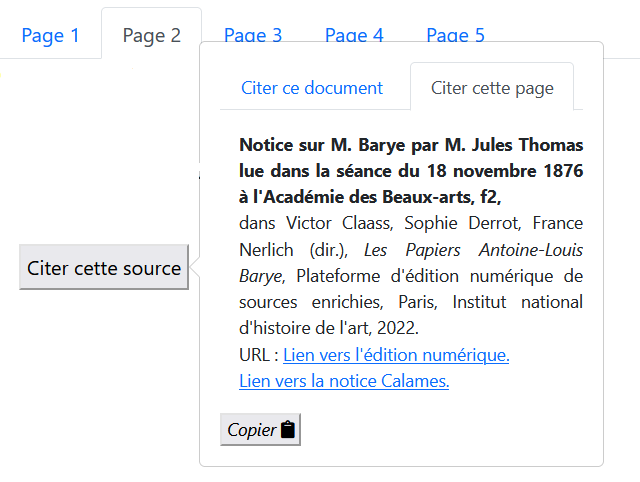
\includegraphics[width=0.8\textwidth]{bouton_citation_transfo_citation_indiv} 
\caption{Prototype de bouton de citation (page de test) tel que produit à l’issue de trois semaines de processus itératifs dans le cadre du stage.} 
\label{fig:prototype-bouton} 
\end{figure}

Les étapes de conception de cet outil suivent les trois phases du \textit{design thinking} décrites par Brown : « inspiration », « idéation » et « implémentation » \footcite[p.5]{brown_design_2008}. Dans un premier temps, les besoins des utilisateurs ont été identifiés, puis conceptualisés sous forme de modélisations, avant d’être finalement implémentés dans une solution fonctionnelle prototypée ayant fait l’objet de plusieurs améliorations accueillant les suggestions émises par le chercheur à l’origine de la demande. 

\subsubsection{Prendre en compte les besoins de l’utilisateur (« empathie »)}

La première étape du processus de \textit{design thinking} consiste à recueillir des informations précises en dialogue avec l’utilisateur final, ici représenté en la personne du chercheur, pour mieux comprendre ses besoins. Ce processus repose sur l’écoute attentive et sur une évaluation équilibrée entre le souhait exprimé par le client et les contraintes techniques ou de faisabilité qui peuvent en découler. Comme le souligne Tim Brown, cette approche est indispensable pour s’assurer que le résultat final correspond non seulement aux attentes, mais qu’il soit également viable dans un contexte de mise en œuvre réelle\footcite{brown_design_2008}.
Dans le cadre du projet \pense, la collecte des informations s’est effectuée sous la forme d’une série de réunions, notamment une réunion initiale, au cours de laquelle le chercheur a pu formuler ses demandes. Une demande spécifique a émergé concernant l’ajout d’un bouton sous forme de pop-over, évoqué plus haut. Celui-ci devait contenir deux onglets : un pour générer une citation l’échelle du document et l’autre à l’échelle de la page individuelle sélectionnée. De plus, un format précis de citation bibliographique a été requis afin de permettre aux utilisateurs de citer facilement les documents présents dans l’édition numérique.
\newline
\textbfit{Familiarité}\\

Comprendre l’usage que les chercheurs font de ces outils constitue une dimension essentielle du \textit{Design Thinking}. Il s’agissait ici de comparer les outils analogues existants sur d’autres plateformes familières aux chercheurs, telles qu’\textit{OpenEdition}, afin d’évaluer les bonnes pratiques en termes d’ergonomie et de proposer une solution facilement appropriable par l’utilisateur ciblé. Parmi les critères analysés figuraient l’intelligibilité de l’outil, sa praticabilité et son assimilation à des codes communs, comme celui du « clipboard », ou presse-papier. En exploitant cette familiarité, l’objectif est de s’assurer que l’utilisateur puisse naviguer aisément dans l’outil, sans avoir besoin de réfléchir excessivement à son fonctionnement – un principe cher au consultant UX Steve Krugs dans son ouvrage intitulé \textit{Don't Make Me Think }.
\newline
\textbfit{Intérêt scientifique de l’outil}\\

Un autre point fondamental à prendre en compte dans la conception de cet outil est son intérêt scientifique, et plus particulièrement la question de la citation. Rendre une édition numérique aisément « citable » est un facteur essentiel pour la diffusion et la reconnaissance scientifique de cette dernière\footcite{sahle_what_2016}. En effet, l’acte de citation permet non seulement de certifier la légitimité d’un document scientifique, mais aussi de favoriser sa réutilisation par la communauté académique, contribuant ainsi à la circulation du savoir. Il s’agit donc de faciliter au maximum l’intégration de l’édition numérique dans le paysage des productions en humanités numériques – un enjeu de taille.
\newline
\textbfit{Réunions régulières pour affiner le projet}\\

Le processus de création de cet outil s’est déroulé de manière itérative, avec des réunions régulières organisées entre les chercheurs, les concepteurs et les ingénieurs. Cette démarche rappelle les méthodes de « co-conception centrée-utilisateur » observées dans d’autres projets comme \textit{Vega}, où les réunions permettent d’ajuster continuellement le prototype afin de mieux répondre aux attentes des utilisateurs\footcite{vial_tournant_2016}. Des réunions effectuées le 15 avril, le 21 et le 29 mai ont été effectuées afin de corriger les prototypes présentés et garantir leur bonne correspondance aux attentes de la recherche.
Parmi les réunions-clés, celle du 15 avril fut dédiée à l’ajustement des aspects formels, tels que l’italique, la longueur des citations, le format de déploiement des URL, l’intégration de liens externes pointant vers les ressources archivistiques (\textit{Calames}) et l’usage d’une virgule plutôt que par des parenthèses pour la séparation de l’URL avec le reste de la citation. Ces ajustements sont essentiels pour s’assurer que les utilisateurs puissent intégrer les citations sans devoir effectuer des corrections manuelles par la suite, garantissant ainsi une cohérence entre les exigences scientifiques et l’ergonomie de l’outil.
Le 21 mai, en préparation de la réunion de pilotage, d’autres éléments formels ont été discutés, notamment la dimension design (volonté d’encadrer les citations) et la nécessité d’adapter les boutons de citation aux parcours spécifiques de l’édition \textit{Barye}, étendant donc l’usage de l’outil au-delà de l’édition des documents manuscrits, en l’intégrant aux commentaires critiques. Une réflexion linguistique a également été menée sur l’usage ou non de l’article démonstratif (« Citer \textit{ce} document » contre « Citer \textit{le} document ») et son impact sur la bonne ergonomie de l’outil. 
\newline
\textbfit{Apport de l’interdisciplinarité}\\

Le processus de conception ne se limitait pas à une approche technique, mais impliquait également une réflexion interdisciplinaire. La réunion du comité de pilotage de \pense du 29 mai illustre cette dimension, en réunissant des experts issus des domaines de l’archivistique, de la bibliothéconomie et des sciences humaines, permettant d’apporter un regard extérieur bienvenu sur la mise en œuvre de l’outil. Ces discussions ont permis d’aborder des questions terminologiques, comme l’usage des termes « feuillet », « page » ou « vue » pour désigner les possibles subdivisions présentes à l’échelle du document, qui selon la matérialité des documents cités et le point de vue adopté sur l’édition, peuvent s’avérer impropres sur le plan archivistique. 

\subsubsection{Modéliser les fonctionnalités attendues (« conceptualisation »)}

Une fois les besoins de l’utilisateur clairement identifiés, la modélisation des fonctionnalités attendues constitue l’étape suivante du processus de conception. Cette phase permet notamment de s’assurer que les parties prenantes – chercheurs, ingénieurs et autres collaborateurs – partagent une vision commune du projet. L’esquisse de storyboards rudimentaires permet ainsi de représenter graphiquement les idées, et vise à dissiper d’éventuelles incompréhensions susceptibles d’émerger à partir des échanges oraux ou des instructions écrites. Ces storyboards, inspirés de l’industrie cinématographique, servent de support visuel aussi bien aux collaborateurs techniques qu’au « client », ici, le chercheur. Une modélisation rudimentaire permet ainsi de vérifier que toutes les parties prenantes sont alignées sur les mêmes objectifs, tout en mobilisant des ressources moindres qu’un véritable prototype.

\subsubsection{Créer, tester et affiner\footnote{« iterative cycles of prototyping, testing and refinement » in \footcite[p.4]{brown_design_2008} (« prototypage »)}

Le processus de développement d’un projet numérique tel que \pense suit une approche caractérisée par des cycles itératifs de création, de test et d’affinement progressif, en cohérence avec les principes du \textit{Design Thinking}. 
Les réorientations successives du projet illustrent cette dynamique. Dans une première phase, une solution entièrement implémentée en JavaScript avait été ainsi envisagée, motivée par la grande flexibilité permise par ce langage. Celle-ci avait pour objectif d’intégrer dynamiquement des feuilles de style XSLT (permettant l’extraction des données textuelles de la base de données \tei et leur transformation en \html « exposable » sur le Web) au JavaScript à travers des requêtes AJAX. Toutefois, cette proposition n’a pas été retenue, ayant été jugée trop complexe et peu adaptée à l’architecture technologique préconisée par l’ingénieur en charge du projet, dans laquelle l’intervention de JavaScript doit se situer en aval, c’est-à-dire au moment du chargement de la page dans le navigateur, et non dans l’interaction avec le serveur (traduisant une approche plus traditionnelle dans l’usage de ce langage). Tandis que des technologies comme XSLT sont davantage employées côté serveur, en amont, pour transformer des données structurées, telles que des documents \xml, avant leur affichage dans le navigateur. Cette séparation des rôles technologiques a donc conduit à une révision de la stratégie initiale adoptée pour le projet \pense. 
\newline
\textbfit{Scripts élaborés}\\

Plusieurs scripts ont été élaborés, essentiellement en XQuery et Python. Les scénarios de transformation XSLT/XQuery visaient à extraire, en temps réel, les informations nécessaires depuis la base de données et à les intégrer sous forme de citations prêtes à l'emploi. Deux approches ont été explorées dans ce cadre : d'une part, la transformation de données en \html accompagnée de code JavaScript, et d'autre part, leur intégration dans des modèles \html préexistants.
Les scripts développés pour la gestion du bouton de citation étaient conçus pour répondre aux besoins spécifiques du projet tout en tenant compte des contraintes techniques imposées par le format des données sources. Les langages utilisés, XQuery et XSLT, se sont révélés adaptés pour manipuler des documents \xml complexes.

Dans le cadre du traitement des fichiers \xml au format \tei, plusieurs scripts intermédiaires ont dû être créés pour répondre à des besoins spécifiques de pré-traitement et d'alignement des données. L’un des premiers scripts développés visait à corriger un problème récurrent dans les fichiers \tei : la présence d’espaces insécables. Ces caractères invisibles provoquaient des erreurs dans le traitement automatique des données. Pour y remédier, un script en Python a été créé pour automatiser leur suppression, normalisant ainsi les fichiers avant leur traitement ultérieur.
Un autre défi technique important a été l’alignement des identifiants entre deux documents \xml distincts et de grammaire différente (\tei et \ead), afin de permettre une mise en concordance des identifiants adossés aux fichiers de la base de données \xml-\tei de \pense avec les identifiants des archives matérielles correspondantes de la base Calames (dont la description est structurée en \xml-\ead, standard pour l’encodage d’inventaires archivistiques). Calames, le \textit{Catalogue en ligne des archives et manuscrits de l’enseignement supérieur}, utilise un système de cote différent de celui adopté en interne par \pense. La principale difficulté résidait dans la différence de granularité entre les identifiants \ead et \tei (les identifiants \tei étant plus précis que les identifiants \ead). Cependant, les deux types de documents partageant une structure arborescente commune, fondée sur le \xml, il a été possible d'utiliser des outils comme XQuery et des bibliothèques Python (telles que \textit{lxml} et \textit{ElementTree}) pour traiter cette correspondance.
Le script développé pour cette tâche avait pour objectif d’automatiser l’extraction des identifiants \tei et leur transformation afin de les aligner avec les identifiants \ead. Le processus débute par l'extraction des identifiants \tei depuis les fichiers correspondants grâce à la bibliothèque \textit{lxml}. Une fois extraits, ces identifiants sont ensuite transformés pour correspondre au format des identifiants \ead. Cette transformation se fait principalement par la normalisation des chaînes de caractères, en supprimant les zéros initiaux et en reformulant la structure des identifiants afin qu’ils soient plus compatibles avec les conventions de nommage du document \ead.
Le script permet ensuite de comparer les identifiants \tei normalisés avec les identifiants \ead, en effectuant une correspondance basée sur une comparaison caractère par caractère. Un algorithme de recherche du « meilleur match » est employé pour déterminer les correspondances les plus précises possibles entre les deux ensembles d’identifiants. Finalement, les résultats de cet alignement sont exportés dans un fichier \csv pour une exploitation future. Ce script constitue une étape importante dans l'enrichissement des métadonnées associées aux documents traités, facilitant ainsi l’intégration du bouton de citation.
\newline
\textbfit{Validation, visualisation et tests}\\

La phase de prototypage, en complément avec la modélisation conceptuelle, étant primordiale pour s’assurer que les solutions proposées répondent aux besoins des utilisateurs finaux, c’est dans cet esprit qu’ont été préparés deux documents destinés à une présentation devant le chercheur principal du projet le 15 avril. Ces documents avaient pour objectif de démontrer l’état d’avancement du prototype du bouton de citation, en particulier sur les aspects liés à l’affichage des données textuelles et à la visualisation des informations sous forme de « cartes ».
Bien que les codes produits à ce stade n’étaient pas conçus pour être des produits finis\footcite[p.3]{brown_design_2008}, ils permettaient d’avoir une vue d’ensemble du système en développement et de tester différentes configurations. Une visualisation par cartes utilisant le \textit{framework} \textit{Bootstrap} a notamment été proposée pour identifier rapidement les anomalies typographiques présentes dans les données textuelles extraites de la base et utilisées pour la citation ; ainsi que les éventuels problèmes dans l’affichage des citations.
Cette étape a permis d’affiner les choix de conception en fonction des retours du chercheur, confirmant ainsi l’adéquation entre les besoins du projet et les solutions technologiques mises en œuvre. De plus, cette démarche s’inscrit dans une logique itérative qui consiste à ajuster continuellement les solutions en fonction des retours des utilisateurs.
            
        \sautdepage

    %% PARTIE III %%
    \part{Dimension expérimentale du projet PENSE : étude des perspectives offertes par l’intelligence artificielle pour l’édition numérique}

        %% Chapitre 6 %%
        \hypertarget{chap6}{%
        \chapter{L’IA au service de l’édition numérique savante, rapide tour d’horizon des applications possibles}\label{chap6-ia}}

            L’intelligence artificielle (IA), notamment sa dimension générative, fait l’objet d’un intérêt croissant depuis l’avènement des grands modèles de langage génératifs, comme celui développé par OpenAI avec ChatGPT, qui facilitent considérablement les interactions entre utilisateurs et modèles d’IA. Bien que ces systèmes aient contribué à une médiatisation intense et à une certaine « démocratisation » de l’IA, il est important de souligner que celle-ci ne se limite pas à ces applications spécifiques. En effet, l’intelligence artificielle représente un champ bien plus vaste (absolument non restreint à l’IA neuronale dont les modèles génératifs cités plus hauts tendent à devenir des emblèmes bien connus du grand public) et ancré dans une histoire longue et complexe. 
Au sein des humanités numériques, l’usage de l’IA se concentre essentiellement sur l’analyse textuelle (dont traitement automatique de la langue) et l’analyse d’image (forme du traitement du signal\footcite[p.98]{sauret_intelligence_2022}), qui figurent parmi les quatre principaux piliers de ce que Olivier Bonfait et ses collaborateurs appellent la « \textit{computational art history}\footcite[p.6]{bonfait_humanites_2021}, une approche qui s’inscrit dans un cadre méthodologique où les technologies numériques transforment la recherche en histoire de l’art. 

\subsection{Histoire (non exhaustive) de l’intelligence artificielle}
\subsubsection{La naissance d’un concept}

La notion d’intelligence artificielle, telle que nous la comprenons aujourd’hui, a pris forme dès le milieu du XXe siècle. Marvin Minsky, l’un des pionniers du domaine, décrivait l’IA comme la « construction de programmes informatiques qui s’adonnent à des tâches qui sont, pour l’instant, accomplies de façon plus satisfaisante par des êtres humains car elles demandent des processus mentaux de haut niveau tels que l’apprentissage perceptuel, l’organisation de la mémoire et le raisonnement critique »\footcite{puren_intelligence_2020}. 
Dans la même veine, Yann LeCun, autre figure de l’IA, précise que son objectif est de « faire faire aux machines des activités que l’on attribue généralement […] aux humains »\footcite{saporta_breve_2018}. 
Ces définitions qui soulignent d’abord le caractère imitatif de l’IA avant la notion de dépassement des capacités humaines, entrent en écho avec une question féconde dans le domaine de la science-fiction, source de fantasmes métaphysiques et de réflexions théoriques sur la nature-même de l’être humain, présentes dans beaucoup de cultures (de « l’homme machine » de La Mettrie (1747) au personnage du « golem » dans le folklore juif…) – l’angoisse et l’espoir simultanés qu’inspire l’IA reflètent en partie la tension entre le pouvoir créateur de l’humain et ses limites, voire son impuissance vis-à-vis d’une potentielle future autonomie des machines. 
Le terme « intelligence artificielle » lui-même a été formulé en 1956 par John McCarthy\footcite{bermes_patrimoine_2020} durant un atelier organisé à Dartmouth College et réunissant des scientifiques pionniers de l’IA tels que Minsky, Allen Newell et Claude Shannon\footcite{puren_intelligence_2020}. 
\newline
\textbfit{IA forte et IA faible}\\

La distinction entre IA « forte » et IA « faible » est fondamentale pour comprendre les différentes approches de cette technologie. L’IA forte désigne une machine capable de développer une véritable conscience de soi, de ressentir des émotions authentiques et de produire un raisonnement lui permettant de comprendre les raisons sous-jacentes à ses actions\footcite{puren_intelligence_2020}. Cette ambition dépasse largement la simulation de l’intelligence humaine pour atteindre un niveau de fonctionnement identique à celui du cerveau humain, où la machine serait en mesure d’apprendre de manière autonome et d’adapter son comportement en fonction des nouvelles informations qu’elle acquiert. Cependant, ce type d’IA demeure largement hypothétique et soulève des défis colossaux.
En revanche, l’IA dite « faible » est moins ambitieuse, mais aussi plus réalisable. Elle désigne des programmes capables de raisonner, d’accumuler des informations et de résoudre des problèmes, mais en simulant seulement ces capacités, sans pour autant posséder une véritable « intelligence » \footcite{puren_intelligence_2020}. Cette approche est aujourd’hui celle qui sous-tend la majorité des systèmes d’intelligence artificielle disponibles, y compris ceux utilisés pour le traitement de texte, la reconnaissance vocale ou encore l’analyse d’image.
\newline
\textbfit{Machine learning et deep learning}\\

L’apprentissage automatique, ou \textit{machine learning}, constitue un domaine central de l’intelligence artificielle. Il s’agit de « l’étude et de l’entraînement d’algorithmes » permettant aux ordinateurs d’apprendre à partir de grandes quantités de données et de faire des prédictions. Cet apprentissage peut se faire de manière supervisée, c’est-à-dire avec l’intervention humaine, ou de manière non supervisée, où l’algorithme apprend de lui-même en identifiant des corrélations dans les données\footcite{puren_intelligence_2020}.
Dans l’apprentissage supervisé, l’algorithme est d’abord entraîné sur un ensemble de données fournies par des humains avant d’être appliqué à de nouvelles données non connues. La qualité des résultats dépend alors en grande partie de la qualité des données fournies et de la cohérence de l’entraînement. En revanche, l’apprentissage non supervisé implique une exploration autonome des données par l’algorithme, sans intervention humaine préalable. Ce dernier regroupe et classe les informations de manière autonome, sans avoir été spécifiquement programmé pour résoudre une tâche donnée\footcite{puren_intelligence_2020}.
L’essor du \textit{deep learning} depuis le milieu des années 2010 a représenté une avancée majeure dans le domaine de l’apprentissage automatique. Reposant sur des réseaux de neurones profonds, c’est-à-dire des architectures composées de plusieurs couches de neurones, chacune interprétant les informations de la couche précédente\footcite{puren_intelligence_2020}, ce type d’algorithme connaît de nos jours une certaine expansion en raison de la disponibilité accrue de vastes quantités de données d’entraînement et de l’accroissement des capacités de calcul des machines. En exploitant ces nouvelles ressources, les réseaux de neurones artificiels sont désormais capables d’apprendre de manière quasi autonome à partir des informations qu’ils traitent. 

\textbfit{Objectifs d’origine}\\

Le contexte d’émergence des premières tentatives pour l’élaboration d’une intelligence artificielle est marqué par la guerre froide et notamment la nécessité en découlant de traductions précises, notamment du russe vers l'anglais. L'importance de la traduction en cette période a orienté la recherche vers le traitement du langage humain par des machines. Le « Georgetown-IBM experiment », mené le 7 janvier 1954, illustre cette tendance. Il s'agissait de la première démonstration d'une machine capable de traduire, bien que de manière très limitée, seulement 250 mots et 49 phrases soigneusement choisies du russe vers l’anglais\footcite{puren_intelligence_2020}. Cet événement est souvent cité comme une étape fondatrice dans le domaine de la traduction automatique.
Quelques années plus tard, en 1968, le gouvernement américain crée la société Systran (System Translation), un projet encore plus ambitieux\footcite{puren_intelligence_2020}. Ces initiatives trouvent plus tard leur apogée dans l'émergence de la traduction statistique dans les années 1980, rendue possible par l'utilisation de grands corpus alignés bilingues. Ces développements ont façonné durablement les recherches en \tal.
Parmi les avancées significatives dans le domaine de l'intelligence artificielle (IA), l'introduction des réseaux de neurones convolutifs (\cnn) dans les années 1990 occupe une place prépondérante\footcite{puren_intelligence_2020}. Ces réseaux permettent d'assembler des informations en couches successives de « neurones », chaque couche recevant et interprétant les informations transmises par la couche précédente\footcite{puren_intelligence_2020}. Ce modèle supposément biomimétique a jeté les bases de nombreuses applications modernes, notamment dans la reconnaissance d'images et le traitement du langage. Toutefois, il convient de rappeler que l’image du « réseau de neurones » n’est qu’une analogie, comme le souligne \citeauthor{sabah_intelligence_2004}Gérard Sabah\footcite[paragraphe 87]{sabah_intelligence_2004}.  En effet, la connaissance actuelle du fonctionnement du cerveau humain est encore partielle, et l’analogie entre les réseaux de neurones artificiels et biologiques repose davantage sur une représentation simplifiée que sur une réalité scientifique.

\subsubsection{Courants symboliques et connexionnistes}

L'intelligence artificielle a connu des périodes de recherche marquées par deux approches dominantes : l'IA symbolique et l'IA connexionniste. Ces paradigmes s'opposent dans leurs principes fondamentaux : l'approche symbolique, ou cognitiviste, repose sur un raisonnement déductif et logique, empruntée au raisonnement humain conscient, tandis que l'approche connexionniste privilégie un raisonnement inductif, « basé sur l'expérience » \footcite[p.7]{bensamoun_rapport_2020}. Le \textit{deep learning}, appartenant au modèle connexionniste, marque le triomphe de cette approche, qui a pourtant connu une certaine mise à l’écart dans les décennies précédentes.

\textbfit{IA symbolique}\newline

L'IA symbolique, parfois surnommée « bonne vieille IA » (\textit{good old fashioned AI} ou GOFAI), se base sur des moteurs de règles et des systèmes experts. Cette approche repose sur un raisonnement formel, logique et explicable, rendant chaque étape du processus suivi par la machine compréhensible par l’humain. Parmi ses pionniers, on retrouve des chercheurs influents tels que Hubert Gelrnter, Allan Newell, Herbert Simon, John McCarthy, James Slagles et Thomas Evans qui ont contribué à poser les fondements d'une IA capable de manipuler des symboles et de résoudre des problèmes complexes par la mise en œuvre de règles prédéfinies\footcite{ezratty_que_nodate}.

\textbfit{IA connexionniste}\newline

En opposition à l'approche symbolique, le connexionnisme est fondé sur des réseaux neuronaux inspirés du fonctionnement biologique du cerveau humain. L'article fondateur de cette approche, intitulé « A logical calculus of the ideas immanent in nervous activity » (1943) et écrit par Warren McCulloch et Walter Pitts, marque un tournant majeur dans l'histoire de l'IA et l’acte de naissance du mouvement connexionniste selon Gilbert Saporta\footcite[p.3]{saporta_breve_2018}. Le \textit{perceptron} de Franck Rosenblatt en 1957-1958, algorithme d’entraînement supervisé spécialisé pour des tâches de classification linéaire (c’est-à-dire de division de données en « classes »), un réseau de neurones dit « simple » et présenté comme la première « machine à apprendre », et constitue l'une des premières implémentations formelles de cette approche\footcite[p.3]{saporta_breve_2018}. Le \textit{perceptron} et ses variantes plus complexes (comme les réseaux multicouches) sont des exemples classiques de réseaux de neurones artificiels, ancrés dans l’approche connexionniste, qui cherchent à simuler certains aspects des réseaux neuronaux « biologiques » (en s’appuyant sur le traitement distribué de l'information à travers des réseaux d'unités simples et interconnectées – comme des neurones).
Cette approche, bien que performante, est souvent critiquée pour son manque d'explicabilité, et ses « boîtes noires », rendant parfois difficile l'interprétation des résultats obtenus. Elle repose sur des méthodes probabilistes, notamment dans des domaines comme la reconnaissance d'images, où les solutions proposées se traduisent par des « pourcentages de véracité » plutôt que des certitudes formelles\footcite{ezratty_que_nodate}.

\textbfit{Opposition entre symbolistes et connexionnistes}\newline

L'opposition entre ces deux courants de l'IA s'illustre par la division entre les \textit{neats}, partisans des méthodes symboliques, et les \textit{scruffies}, adeptes des méthodes connexionnistes, comme le rappelle Olivier Ezratty\footcite{ezratty_que_nodate}. Alors que l'approche symbolique privilégie la logique formelle et l'explicabilité, le connexionnisme est souvent perçu comme une « boîte noire », difficile à déchiffrer. Cependant, ces deux courants ne sont pas totalement irréconciliables, comme le souligne Olivier Ezratty, qui fait une analogie entre les façons dont les humains et les machines apprennent. Ainsi, un humain peut apprendre à la fois par la lecture et l’apprentissage de règles formelles (symbolisme) et par l'expérience empirique (connexionnisme). Ces deux modes d'apprentissage sont complémentaires : l'un traite les flux d'information, tandis que l'autre exploite le stock de connaissances acquises\footcite{ezratty_que_nodate}.

\textbfit{Le connexionnisme peut-il parvenir à dépasser le \emph{semantic gap} ? }\newline

Une question majeure dans le domaine du traitement computationnel du langage naturel, reste à savoir si le connexionnisme peut combler le « \textit{semantic gap} », concept rappelé par Lev Manovich et désignant l'écart entre la manière dont un humain extrait et traite des informations et la manière dont une machine le fait\footcite[p.22]{manovich_data_2015}. Ce problème est particulièrement prégnant dans le domaine de la pragmatique, une composante de la linguistique traitant de l'interprétation contextuelle du langage, et qui demeure aujourd'hui l'une des parties les plus complexes à transposer en algorithmes\footcite[p.19]{yvon_petite_2007}, qu’ils soient d’origine symbolique ou connexionniste.

\textbfit{Hivers de l’IA}\newline

L'histoire de l'IA est ponctuée de périodes dites « hivers », où les recherches stagnent, voire sont abandonnées. Pour l'IA connexionniste, le premier hiver a eu lieu entre 1970 et 1980, suite à la démonstration des limites du \textit{perceptron}\footcite{saporta_breve_2018}. Un deuxième hiver intervient à partir de la fin des années 1980, en raison de l'insuffisance des capacités de calcul nécessaires pour développer des réseaux neuronaux plus complexes\footcite{saporta_breve_2018}.
L'IA symbolique, quant à elle, connaît également ses périodes de recul, notamment depuis une quinzaine d’années. L'une des principales raisons réside dans « l'inadéquation de ses méthodes pour le traitement du langage », champ de recherche majeur en IA, ainsi que dans la difficulté à « collecter et structurer [de manière exhaustive] les règles du savoir humain » \footcite{ezratty_que_nodate}.

\textbfit{IA générale et IA forte}\newline

Un autre sujet de débat concerne la distinction entre IA générale (AGI) et IA forte, souvent confondues. L’IA générale, qui ferait preuve de capacités d’adaptation et de raisonnement comparables à celles de l'intelligence humaine, est encore loin d’être réalisée. Les débats à ce sujet restent vifs, et il est probable que la solution réside dans une combinaison des approches connexionnistes et symboliques selon Olivier Ezrarry\footcite{ezratty_que_nodate}.

\subsubsection{Applications possibles dans les GLAM (Galleries, Libraries, Archive, Museums) et dans les institutions de recherche}

Les humanités numériques (HN) bénéficient de nouvelles méthodes de traitement des données, notamment grâce à la data science, qui devient un outil essentiel pour gérer les grandes volumétries d’informations auxquelles sont confrontées les institutions patrimoniales. Par exemple, dans les musées, bibliothèques et archives, l’utilisation de techniques avancées de traitement de données permet non seulement de traiter des volumes massifs d’informations\footcite{bermes_patrimoine_2020}, mais aussi d’aborder de manière plus nuancée des volumes plus restreints\footcite[p.29]{manovich_data_2015}. 
Le concept de \textit{distant viewing} s’inscrit dans cette perspective. Adapté du \textit{distant reading} de Franco Moretti, ce concept se concentre sur l'analyse à grande échelle d'objets picturaux, en permettant de traiter des ensembles d’images de manière collective, plutôt qu’individuelle. L’IA, combinée aux pratiques de la science des données, offre des possibilités sans précédent pour traiter des volumes massifs d’images, ce qui est devenu indispensable après les réflexes de numérisation massive engagés dès les années 1990 et par l’explosion des productions d’archives nativement numériques\footcite{arnold_distant_2019}.
Un autre exemple frappant de l'application de l'intelligence artificielle (IA) dans le domaine du patrimoine est la reconstruction d'œuvres d'art dégradées ou disparues, dont nous ne disposons que de photographies de mauvaises qualités, comme les œuvres citées par David Stork\footcite[p.685-87]{stork_how_2023}, grâce au \textit{deep learning}. Toutefois, il est important de noter que la qualité des résultats dépend fortement de l'entraînement du modèle et des compétences en histoire de l'art mobilisées lors de cette phase d’apprentissage. En effet, la machine peut produire une hypothèse statistiquement plausible, mais historiquement inexacte. Il s'agit d'un domaine où la collaboration entre ingénieurs et chercheurs devient alors essentielle pour garantir la pertinence du résultat obtenu. Le dialogue entre ces deux groupes est indispensable pour que les ingénieurs, souvent perçus comme responsables des aspects techniques, et les chercheurs, experts du contenu, puissent conjointement interpréter les résultats produits par l’IA. En effet, L’ingénieur seul, à moins d’être lui-même un spécialiste (« un historien [de l’art] programmeur », pour reprendre la phrase d’Emmanuel Le Roy Ladurie\footcite{lemny__2017}) ne peut saisir toutes les nuances complexes à prendre en compte.
Enfin, il convient également de noter que l'IA n'est pas l'unique facteur ayant entraîné des changements de paradigmes en histoire de l'art. Comme l'expliquent Aubry, Costner et James, l'IA est certes un vecteur de transformation, mais elle ne fait que s’inscrire dans une tendance plus large qui inclut l’évolution des technologies numériques et les pratiques de recherche associées\footcite[p.59]{aubry_artificial_2021}.

\subsection{Perspectives offertes par la « vision par ordinateur »}

\subsubsection{Traitement de l’image picturale}

Dans le cadre du traitement d’images picturales, l'intelligence artificielle permet d'extraire, d'identifier et de segmenter des éléments spécifiques au sein des œuvres d'art. Le processus commence par l'extraction des données visuelles d'une image, qui est ensuite soumise à un algorithme de reconnaissance, spécialement entraîné pour l’identification de certains motifs. Celui-ci est capable de détecter des formes, des couleurs et des motifs, permettant ainsi la classification des différents éléments picturaux. La segmentation joue un rôle clé dans ce traitement en divisant l’image en plusieurs segments, chacun représentant une composante spécifique, telle qu’un personnage ou un objet. 
Dans le cadre du projet \pense, une partie du corpus Karbowsky a été traitée par des méthodes de segmentation manuelle. Cependant, l’ambition à long terme est d’automatiser cette tâche (pour les corpus qui s’y prêtent !), afin d’accélérer le processus d’analyse d’un corpus particulièrement vaste. Cela permettrait de traiter non seulement un volume important d'images, mais également d’appliquer ces techniques à des corpus hétérogènes de manière plus systématique.

\subsubsection{Traitement de l’image comportant du texte}

L’application des techniques d’intelligence artificielle au traitement de l’image contenant du texte est une composante fréquemment retrouvée dans les projets d’édition numérique. Le développement de l'\ocr et de l'\htr a permis une amélioration significative de la transcription automatique des documents. Ce processus se décompose en plusieurs étapes : tout d’abord, la segmentation permet de localiser les blocs de texte sur une image. Ensuite, une analyse de la mise en page (organisation logique des blocs) peut être effectuée pour organiser ces segments. Enfin, la transcription automatique (basée sur la reconnaissance de pixels) convertit les caractères identifiés dans chaque bloc en texte numérique\footcite[p.3]{chague_htr-united_2022}. Ces tâches reposent sur des techniques d'apprentissage supervisé ou non-supervisé, nécessitant l'entraînement de modèles spécialisés à partir de larges volumes de données d'exemple. Il existe de fait une grande proximité technique entre l’\htr et l’\ocr, les deux technologies partageant des principes similaires\footcite[p.5]{biay_chaine_2022}. Enfin, signalons que d’autres applications voisines existent,  comme \textit{l’Optical Layout Recognition} (OLR) et \textit{l’Optical Musical Recognition} (OMR). L'OLR s’intéresse à l’identification des structures de mise en page au sein des documents visuels, tandis que l’OMR se concentre sur la reconnaissance de partitions musicales\footcite[p.91]{bermes_patrimoine_2020}.

\subsection{Applications possibles en traitement automatique de la langue}

Le traitement automatique de la langue (TAL) est une discipline de plus en plus centrale dans les projets d'édition numérique, particulièrement ceux qui visent à automatiser et enrichir l'analyse des corpus textuels. En termes simples, le TAL se concentre sur le développement d'algorithmes capables de traiter, d'analyser et de comprendre les langues humaines naturelles à travers des processus automatiques. Parmi les applications notables dans ce domaine, on retrouve des tâches comme la reconnaissance d'entités nommées, qui permet l'identification automatique de noms propres (personnes, lieux, organisations) dans un texte. Cela facilite grandement l'indexation automatique des données et la cartographie des relations entre différents éléments au sein des corpus, des outils présentant un intérêt non négligeable pour des éditions numériques dans le domaine des humanités numériques, ou dans une approche différente, pour les instruments de recherche archivistique comme cela été l’objet du projet \textit{NER4Archives} par exemple\footnote{Voir pour cela : https://hal.science/hal-03625734}. D'autres tâches plus traditionnellement rattachée à l’analyse linguistique, comme l'étiquetage grammatical (ou \textit{POS tagging}) et la lemmatisation, qui permettent respectivement de catégoriser les mots par leur fonction et de réduire les mots à leur forme « canonique », peuvent s’avérer utiles dans les processus de pré-traitement textuel pour les éditions numériques\footnote{Sur l’évolution du TAL vers l’IA, voir : \footcite[paragraphe 17]{leon_histoire_2015}}.

\subsubsection{Textométrie et analyse statistique de la langue}

\textbfit{Une approche ancienne}\newline

L’analyse statistique et quantitative de la langue est l'une des premières approches historiquement associées au développement des humanités numériques. Elle est souvent assimilée à l'\ia symbolique, en raison de sa dimension systématique et quantitative. Le travail de Roberto Busa est fréquemment cité comme l'un des premiers exemples d'application de méthodes computationnelles dans l'analyse des textes. En tant que précurseur des humanités numériques, Busa a employé des techniques lexicographiques pour établir des concordances dans les corpus, préfigurant en cela, selon Pierre Mounier, le concept de \textit{distant reading} de Franco Moretti\footcite[paragraphe 5]{mounier_ibm_2018}. Il paraît cependant anachronique de parler d’usage d’IA symbolique pour le travail qu’a mené Busa, puisque le concept n’était pas encore formulé (1956) lorsqu’il débuta en 1949 son entreprise computationnelle. Il semble cependant s’être appuyé sur un système basé sur des règles statistiques, système qui, en évoluant, a été rattaché au mouvement symbolique de l’intelligence artificielle. Comme l'a noté Mounier, bien que le concept d'IA symbolique n'ait pas encore été formulé à l'époque, le travail de Busa s'appuyait déjà sur un système de règles statistiques, anticipant ainsi certaines des méthodes modernes d'analyse des corpus.
\newline
\textbfit{La textométrie, une formalisation de l’approche statistique des textes}\\

La textométrie, qui constitue l’une des approches du traitement statistique des corpus textuels, s'est principalement développée en France à partir des années 1970, avec les travaux de Pierre Guiraud, Charles Muller et de Jean-Paul Benzécri. Il s’agit de quantifier et de visualiser les relations entre les mots et les textes\footcite{pincemin_quest-ce_2008}, permettant ainsi de repérer des patterns lexicaux ou structurels au sein des corpus. Les résultats de ces analyses permettent non seulement de produire des visualisations cartographiques des textes, mais aussi d'interpréter les données sous la forme de regroupements et de mises en évidence de termes clés à travers les corpus  \footnote{Voir également \footcite{pincemin_textometrie_2020}}. 
Malgré l'importance de cette discipline, son usage dans les éditions numériques (bien que théoriquement facilitée par la compatibilité de la plateforme TXM avec le format \tei par exemple\footcite{noauthor_txm_2019}), notamment dans le domaine de l'histoire de l'art, reste relativement limité. Comme l'a observé Emmanuel Château-Dutier, l'application de la textométrie et de l'analyse du discours dans les éditions numériques en histoire de l'art demeure encore à explorer ; situation pouvant partiellement s’expliquer par la relative moindre attention portée au texte en histoire de l’art, au bénéfice de l’image\footcite[p.86]{chateau-dutier_editions_2021}.
\newline
\textbfit{La lecture distante et le traitement de corpus massifs}\\

Un autre concept clé dans ce champ est celui de la « lecture distante » (ou \textit{distant reading}), proposé par Franco Moretti en 2000. Ce dernier a développé cette approche comme une alternative à la lecture dite « proche » (ou \textit{close reading}), qui privilégie une analyse approfondie d'un texte singulier. À l'inverse, la lecture distante consiste à analyser de vastes bases de données textuelles, souvent constituées de milliers de textes, dans le but de détecter des motifs récurrents (des \textit{patterns}) ou des structures « qui traversent les siècles et les frontières » \footcite{puren_intelligence_2020} afin de dégager des tendances littéraires sur le long terme. Pour Moretti, les méthodes classiques d'analyse littéraire souffrent d'un biais, en se concentrant exclusivement sur des auteurs appartenant au canon littéraire, excluant de fait une grande partie de la production textuelle de leur époque\footcite[paragraphe 12]{mounier_ce_2018} ; la lecture distante entend ainsi combler ce manque par l’analyse de corpus massifs, assistée de nos jours par méthodes computationnelles, qu’elles soient statistiques, issues de la textométrie ou d’autres approches voisines (la fouille de texte ou l’analyse sémantique latente, sur lesquelles nous ne nous attarderons pas ici), ou neuronales, par le recours aux capacités de classification d’un grand modèle de langage par exemple.

\subsubsection{La correction automatique de texte : de l’IA symbolique au \textit{deep learning}}

La correction de textes revêt une importance scientifique centrale dans le cadre d’une édition critique, particulièrement pour des projets visant à produire une version intelligible et fluide d’un texte en éliminant les scories qui en entravent la lecture, telles que les ratures, hésitations graphiques, ou encore erreurs variées. La tradition éditoriale critique tend à présenter un texte corrigé et « normalisé » selon les conventions orthographiques, grammaticales et de mise en forme contemporaines de l’époque de la publication\footcite{nougaret_ledition_2015}. Dans le cadre du projet \pense, nous nous sommes intéressés à la question de la post-correction orthographique et syntaxique du corpus de correspondance Doucet - René-Jean, successive à la production d’une transcription manuelle imitative ayant scrupuleusement respecté la forme d’origine, comprenant de nombreux écarts par rapport aux conventions d’écriture du XXIème siècle. Plus précisément, il s’agissait de s’interroger sur les possibilités offertes par un grand modèle de langage en ce qui concerne cette tâche de correction.
La correction automatique a suivi une évolution importante depuis ses débuts. Dans un premier temps, les correcteurs (ou « correcticiels » \footcite{jacquet-pfau_correcteurs_2001}) étaient basés sur des règles simples, telles que les correspondances exactes de mots, avant de se complexifier avec l’introduction de dictionnaires. Cela a permis d’élargir le champ des corrections, mais cette approche restait limitée aux erreurs directement identifiables par rapport aux normes lexicales et orthographiques. Le développement d’algorithmes de détection plus sophistiqués, comme ceux basés sur des modèles statistiques, a permis de franchir une nouvelle étape, notamment en prenant en compte les probabilités d’apparition des mots dans un contexte donné\footcite{mitton_fifty_2010}. Enfin, les dernières avancées dans le domaine de l’intelligence artificielle ont introduit le \textit{deep learning}, ayant recours à des réseaux neuronaux pour détecter des erreurs plus subtiles.

\textbfit{Usage d’un LLM pour la correction automatique de textes}\newline

Il existe une littérature relativement abondante sur l’usage de grands modèles de langage (\llm) pour la post-correction de texte bruités, c’est-à-dire présentant des anomalies essentiellement d’ordre typographiques, générés par \ocr ou \htr (reconnaissance automatique des caractères, typographiques ou manuscrits). Cependant, avant de plaquer les observations émises dans ces contextes-ci sur le cas de la post-correction que nous avons choisi d’opérer pour le corpus Doucet, il est important de noter une différence importante : le corpus textuel sur lequel nous travaillons est un corpus produit par transcription imitative générée par l’humain. Les anomalies ou erreurs caractéristiques rencontrés dans ce corpus sont donc de nature différente des anomalies rencontrées dans les sorties d’\ocr ou d'\htr. Là où un corpus imitatif reflétera les erreurs spécifiques d’un scripteur, pouvant avoir plusieurs origines (adoption d’une graphie fautive, erreur d’inattention, conventions orthographiques ou syntaxiques appartenant à une époque différente), les erreurs de transcription post-\ocr ou \htr se rapprochent davantage de fautes de frappe, dues à des confusions typographiques\footcite{mitton_fifty_2010}. Par exemple, un texte \ocr est souvent sujet à des erreurs où des caractères similaires sont confondus, comme la lecture d’un double N « nn » au lieu d’un « m » \footcite[p.95]{baranes_vers_2012}.

\textbfit{Fonctionnement d’un LLM pour le traitement du langage}\newline

Un \llm fonctionne très différemment des techniques de correction symbolique traditionnelles. La première étape dans le processus de correction est le prétraitement du texte. Ce prétraitement inclut la tokenisation (découpage du texte en unités distinctes appelées tokens) et la vectorisation desdits tokens. Cette étape consiste à transformer les tokens en vecteurs mathématiques, ce qui permet aux modèles de travailler sur des données numériques\footcite{das_building_2024}. Comme l’explique Ezratty, le \textit{deep learning} ne « comprend » pas le texte au sens humain du terme, mais il génère une représentation mathématique de ce texte, traitant les mots voire les syllabes comme des vecteurs\footcite{ezratty_que_nodate}.  Les calculs de distance entre vecteurs permettent alors de repérer des similarités entre des séquences textuelles.
La deuxième étape clé dans le fonctionnement d’un \llm, tel que GPT de OpenAI est la contextualisation du texte via le mécanisme d'attention. Ce processus repose (pour un \llm tel que GPT) sur une architecture appelée \textit{Transformer}, dans laquelle des couches d'attention (notamment l'attention multi-tête\footcite{noauthor_transformateurs_nodate}) permettent au modèle de « comprendre » le contexte global du texte. Ce mécanisme, appelé « self-attention », permet au modèle de peser l'importance de chaque mot dans une séquence en tenant compte des autres mots qui l’entourent\footcite[p.2]{vaswani_attention_2023}.   Cela donne au \llm une capacité à maintenir un contexte cohérent sur de longues distances dans le texte, contrairement aux approches plus locales des techniques symboliques.
La troisième étape est la génération de la correction, qui repose sur la prédiction probabiliste des tokens les plus appropriés à chaque position dans la séquence. Le modèle propose des substitutions, des réarrangements, ou même la suppression de certains tokens en fonction des probabilités calculées. La différence entre la génération de la correction et la reconstruction du texte réside dans le fait que la génération se concentre sur les changements locaux (à l’échelle du token ou de la séquence), tandis que la reconstruction consiste à valider le texte dans son ensemble pour garantir une cohérence structurelle.
L’utilisation des \llm pour la correction de corpus bruités, comme les textes historiques océrisés, a cependant ses limites. Certaines études indiquent que ces modèles ont tendance à surcorriger, c’est-à-dire à apporter des modifications inutiles ou exagérées. Ce problème peut néanmoins être relativement atténué grâce à des techniques de \textit{prompt engineering}qui permettent d’optimiser les exemples et les instructions donnés au modèle\footcite[p.135]{boros_post-correction_2024}. Comme l’indiquent plusieurs auteurs, il vaut mieux qu'un correcteur automatique sous-corrige plutôt qu'il ne sur-corrige, car la sur-correction altère l'intégrité du texte original, tandis que la sous-correction préserve davantage le texte en dépit de quelques erreurs\footcite[p.2]{baranes_vers_2012}.

\textbfit{Les alternatives aux LLM pour la post-correction côté neuronal : zoom sur les MLM et les modèles Seq2Seq}\newline

Les \mlm sont une autre catégorie de modèles qui peuvent être utilisés pour la correction de textes. Leur fonctionnement diffère des \llm en ce qu’ils s’appuient sur une technique appelée « \textit{masked language modeling}». Ce processus consiste à masquer certains tokens dans une séquence, sous la forme ‘[MASK]’ par exemple, et à demander au modèle de prédire ces tokens manquants en se basant sur le contexte environnant. Parmi les \mlm, citons par exemple CamemBERT, adaptation franco-française du BERT de Google\footcite{martin_camembert_2020}.   Cette approche permet au modèle de comprendre les relations contextuelles de manière plus fine\footnote{Sur le fonctionnement précis des \mlm, voir : Daniel Jurafsky et James H. Martin, « Masked Language Models », in \textit{Speech and Language Processing}, 2024, https://web.stanford.edu/~jurafsky/slp3/11.pdf}.   
Le \textit{Seq2Seq} (\textit{Sequence to Sequence}) est une architecture utilisée pour des tâches de génération de texte, notamment la traduction ou la correction automatique. Contrairement aux \llm, qui utilisent généralement un seul décodeur, les modèles \textit{Seq2Seq} reposent sur une architecture encodeur-décodeur, où l’encodeur transforme une séquence d'entrée en une représentation fixe, et le décodeur génère une nouvelle séquence à partir de cette représentation. Cette approche permet une vision plus globale du texte et une meilleure compréhension des relations entre les tokens, ce qui en fait un outil puissant pour la correction de textes\footcite{sutskever_sequence_2014}. La technique de vectorisation utilisée dans \textit{Seq2Seq}, est également différente de celle des \llm, car elle vise à créer des représentations continues des mots dans un espace vectoriel, en s’appuyant sur la similarité sémantique entre les mots et non seulement sur leur fréquence d'apparition dans les textes. Il semble qu’un modèle \textit{Seq2Seq} aura une vision plus « globale » que celle d’un LLM vis-à-vis du texte pris en entrée pour une tâche de correction. 
            
        \sautdepage

        %% Chapitre 7 %%
        \hypertarget{chap7}{%
        \chapter[Un exemple d’usage de l’IA neuronale en post-traitement de corpus textuels]{Un exemple d’usage de l’IA neuronale en post-traitement de corpus textuels : correction automatique du corpus Doucet par grand modèle de langage (LLM). \\ \ Protocole, résultats et alternatives}\label{chap7-llm-postco}}

            \subsection{Le corpus Doucet : caractéristiques graphiques et objectifs de normalisation}

Avant de nous pencher sur les anomalies récurrentes observables dans le corpus de correspondances (1908-1929) entre Jacques Doucet et René-Jean, ayant fait l’objet d’une transcription imitative\footnote{Voir les chapitres 2 et 4 du présent mémoire.} rappelons brièvement son contexte de production. Il s’agit d’une partie d’un échange épistolaire privé (les lettres expédiées par Doucet et reçues par René-Jean), non destiné à la publication, s’étendant sur une période relativement étendue, et concentré en une assez modeste volumétrie (moins de 100 lettres pour le corpus actuellement traité (2024) par le projet \pense). Ne présentant, pour la majeure partie des documents, qu’un scripteur unique (Doucet), à quelques exceptions très localisées (ajouts manuscrits de René-Jean, numérotation introduite par Sylvie Maignan…), l’écriture est manuscrite, cursive et susceptible de présenter des difficultés à la lecture.

En ce qui concerne la conformité avec les conventions orthographiques et syntaxiques (ponctuation…), un certain nombre d’anomalies récurrentes sont observables dans le corpus, ce qui interroge notamment en ce qui concerne le rapport de Doucet à l’écriture, et plus largement la nature des pratiques d’écriture à l’époque et dans le milieu social de Doucet. On peut se demander s'il s'agit de caractéristiques propres à cette époque ou au processus d'apprentissage de l’écriture tel qu’on l'enseignait aux enfants au moment de l'enfance de Doucet. Cependant, il est difficile de se prononcer de manière définitive, faute de documentation scientifique suffisante sur ce point. Il semble néanmoins pertinent de souligner certains éléments notables.

\subsubsection{Typologies d’anomalies fréquemment rencontrées}

\begin{center}     
\begin{longtable}{|p{5cm}|p{5cm}|p{5cm}|}
    \hline
    \textbf{Type d'anomalie} & \textbf{Exemple} & \textbf{Correction attendue}\endfirsthead \\ \hline
    \textbf{Type d'anomalie} & \textbf{Exemple} & \textbf{Correction attendue}\endhead \\ \hline
    
    Absence d’accentuation ou accentuation inexacte/irrégulière & « il vous expediera » (bnf\_naf13124\_2\_61),\newline « du plus grand interét presentée avec » (bnf\_naf13124\_2\_59) & « il vous expédiera […] »,\newline « du plus grand intérêt présenté avec […] » \\ \hline
    Absence de ponctuation (point et virgule) & « Nous sommes en bonne santé Amitié à tous » (bnf\_naf13124\_2\_61),\newline « vous l'enverra moyennant finance bien entendu c'est un homme precieux pour l'Art chretien. » (bnf\_naf13124\_2\_60) & « Nous sommes en bonne santé. Amitié à tous. »,\newline « vous l’enverra moyennant finances, bien entendu c’est un homme précieux pour l’Art chrétien. » \\ \hline
    Substitution de la virgule par le point & « et de vos bons souhaits. nous revoila » (bnf\_naf13124\_2\_60) & « et de vos bons souhaits, nous revoilà […] » \\ \hline    
    Absence de tirets dans les inversions sujet-verbe & « Avons nous une revue grecque sur l'art chretien » (bnf\_naf13124\_2\_60) & « Avons-nous un revue grecque sur l’art chrétien […] ? » \\ \hline   
    Substitution du point d’interrogation par un point final. & « toutes celles que ce
Simiriottis a pu me livrer sont marquees dans son catalogue joint a l'envoi, il doit completer ce qui manque mais quand. » (bnf\_naf13124\_2\_61) & « toutes celles que ce Simiriottis a pu me livrer sont marquées dans son catalogue joint à l’envoi, il doit compléter ce qui manque, mais quand ? » [hypothèse interprétative] \\ \hline    
    Substitution du point par le tiret & « Faites moi donc creance d'une semaine ou deux - Merci et bien à vous. » (bnf\_naf13124\_2\_52),\newline « j'ai été si pris par les mille choses qu'il faut que je fasse moi-même qu'il ne m'a pas été possible de venir un peu causer avec vous - Je vais bien moral et physique voici pour moi. » (bnf\_naf13124\_2\_49) & « Faites-moi donc créance d’une semaine ou deux. Merci et bien à vous. »,\newline « J’ai été si pris par les mille choses qu’il faut que je fasse moi-même qu’il ne m’a pas été possible de venir un peu causer avec vous. Je vais bien, moral et physique, voici pour moi. » \\ \hline 
    \caption{Typologie des anomalies fréquemment rencontrées dans le corpus Doucet.} % Légende sous le tableau
\end{longtable}   
\end{center}

Premièrement, ces anomalies semblent rappeler un usage de la ponctuation qui pourrait être qualifié d'« oral » ou « à l’ancienne », rappelant des pratiques de l’écriture du XVIIIe siècle, où l’usage de la ponctuation visait à refléter les pauses respiratoires dans le discours oral. Comme le remarque Annette Lorenceau, cette approche de la ponctuation, substituant la virgule par un point et le point final par un tiret par exemple, s'éloigne des règles strictement grammaticales privilégiées au XIXe siècle, se caractérisant par une utilisation plus codifiée et plus abondante (voire excessive, du point de vue contemporain) des signes de ponctuation\footcite[p.51]{lorenceau_ponctuation_1980}. Ce phénomène, observé chez Doucet, pourrait s'expliquer par plusieurs hypothèses aux appuis néanmoins relativement faibles, que nous émettons ci-après. D’une part, la familiarité de Doucet, que l’on sait grand collectionneur d’art du XVIIIème, avec la culture livresque de cette époque, pourrait avoir influencé son écriture. D'autre part, une certaine habitude de la dimension orale des échanges (écrivant à ses destinataires comme il parle à ses collaborateurs) pourrait justifier une écriture proche du langage parlé. Il est également à noter que l’usage du tiret comme d’un point final est notée par Marie-Anne Sarda, chercheuse responsable de l’édition numérique de la correspondance de Doucet, comme « courante » au XIXème siècle\footcite{carius_principes_2024}. Remarquons que dans ce cas précis, il est également possible qu’il s’agisse d’un simple choix de représentation graphique consistant à étendre le tracé du point final jusqu’à le faire ressembler à un tiret.

\subsubsection{Résultat souhaité par la recherche}
Le projet \pense s’inscrit dans une volonté de maintenir une continuité avec les traditions de l’édition papier tout en proposant une expérience de lecture adaptée aux possibilités offertes par le numérique. En s'inspirant des corpus alignés bilingues, comme le montre l'exemple du projet \textit{Architrave}\footcite{noauthor_architrave_nodate}, ainsi que des éditions génétiques, telles que \textit{E-Balzac}, \pense cherche avec l’édition Doucet, nous l’avons déjà dit, à offrir une double lecture : d’une part, une édition diplomatique imitative, respectant la matérialité du manuscrit, et d’autre part, une édition critique plus classique, conforme aux normes modernes d’édition de textes manuscrits\footcite{carius_principes_2024}.
Cette double approche permettrait aux lecteurs de naviguer facilement entre ces deux versions, éventuellement à terme grâce à un système d’onglets interactifs (comme dans l’édition \textit{Architrave}), offrant ainsi une expérience enrichie. 
Il s’agit donc pour l’étape de la correction devant servir de base à l’édition critique, de proposer une lecture facilitée au lecteur : les anomalies les plus fréquemment retrouvées, à savoir les erreurs de ponctuation et d’accentuation, doivent donc faire l’objet d’une normalisation, selon la forme proposée ci-dessus. Pour cela, et en s’inscrivant dans la dimension expérimentale affirmée de \pense, nous avons fait le choix de nous pencher sur les perspectives proposées par l’\ia générative. 

\subsubsection{Présentation des outils choisis}
Nous nous sommes tournés vers l’\api de GPT 3.5, qui s'est avéré être un choix pertinent en raison de sa facilité de prise en main et de sa capacité à traiter des tâches complexes sans nécessiter un entraînement spécifique du modèle. Cette décision a été motivée par des contraintes de temps et d'infrastructure, en lien avec le cadre temporel du projet. Bien que l’utilisation de cette \api soit payante, le coût par token\footnote{Un token, dans le contexte de l’\api GPT, représente une unité minimale de texte, composée de quelques caractères ou mots, utilisée par le modèle pour générer une réponse. Chaque requête envoyée à l’\api se voit facturer en fonction du nombre de tokens consommés (tokens fournit en entrée par l’utilisateur et tokens produits en sortie par l’IA générative) ce qui permet de mesurer la quantité de texte traité lors de chaque opération.} s’est révélé compatible avec les besoins du projet, le corpus à traiter étant d’une volumétrie assez faible. La préférence pour l’\api plutôt que pour l’interface de Chat de GPT se justifie par un meilleur contrôle des paramètres du prompt, les capacités de systématisation (application du prompt à un corpus de plusieurs fichiers) et par la possibilité de produire des fichiers au format TXT directement en sortie. 
En parallèle, Google Colab a été utilisé comme environnement de travail pour faciliter les expérimentations initialement envisagées, avec des modèles plus spécifiques, comme le \mlm CamemBERT, du fait de sa capacité à exploiter des ressources GPU externes (ressources limitées fournies par Google). Ce choix s’explique par le besoin de ressources informatiques supplémentaires, notamment pour des tâches de fine-tuning de modèles. Google Colab, bien que soumis à certaines limitations en termes de temps d’exécution et de ressources, nous permettait alors de surmonter un certains nombres de contraintes. Bien que le recours à un \mlm ait été finalement abandonné du fait de difficultés techniques, nous avons conservé l’usage aux notebooks de Google Colab par confort et ergonomie.

\textbfit{L’enjeu de la réplicabilité}\newline
Un enjeu majeur de l’usage de grand modèle de langage pour des tâches spécifiques concerne la réplicabilité : le modèle étant entraîné avec des données d’apprentissage massives combinées à des milliards de paramètres pouvant apparaître comme peu aisément manipulables, voire comme une véritable « boîte noire » pour l’utilisateur, comment s’assurer que le modèle générera la même réponse au même prompt quelle que soit les conditions ? Pour essayer de limiter les variations, il s’agit de configurer un certains nombres de paramètres dont notamment la température. 
Dans le contexte du \textit{prompt engineering} (que l’on peut définir comme l’ensemble des méthodes, exprimées en langage naturel ou sous forme de code de plus bas niveau, permettant de modeler la réponse fournie par un modèle d’IA générative), la température est un paramètre clé permettant de moduler la créativité d’un modèle de langage. En abaissant la température, on favorise des réponses plus déterministes, où le modèle aura moins tendance à explorer des alternatives variées et créatives (mais aussi plus susceptibles de virer à l’hallucination). En revanche, une température élevée encourage des réponses plus créatives, mais moins prévisibles. Le contrôle de ce paramètre apparaît donc essentiel pour obtenir des résultats reproductibles dans le cadre de l'utilisation des \llm\footcite{reddy_controlling_2024}.
D'autres paramètres, comme le \textit{top-k} et le \textit{top-p}, peuvent également être ajustés pour moduler la sortie générée par le modèle. Le paramètre \textit{top-k} restreint les choix possibles du modèle aux \textbf{k}\footnote{Le « k » dans top-k se réfère seulement à un sous-ensemble des meilleurs éléments.} mots les plus probables à chaque étape de génération, tandis que \textit{top-p} (ou \textit{nucleus sampling}, échantillonnage de noyau) permet de considérer uniquement les mots dont la probabilité cumulée atteint un certain seuil\footcite{weinmeister_beyond_2024}. De même que pour la température, plus les valeurs assignées à ces paramètres sont basses, plus les réponses susceptibles d’être générées seront jugées statistiquement probables. Ces ajustements offrent un contrôle plus fin sur la qualité et la cohérence des résultats produits par le \llm. En les combinant avec la température, il est possible d’influencer la variabilité des réponses tout en maintenant une certaine cohérence dans les sorties.

\subsection{Requêtage de l’API de GPT 3.5 pour la correction automatique de texte non balisé}
\subsubsection{Présentation technique de l’outil}

L’\api GPT 3.5, développée par OpenAI, repose sur un modèle de langage de grande taille (\llm, \textit{Large Language Model}), capable de générer du texte en se basant sur des milliards de paramètres et d'un corpus textuel immense, comprenant notamment une partie du web archivé par l’organisation Common Crawl pour GPT 3\footcite[p.8]{brown_language_2020}. Ces modèles utilisent des techniques d’apprentissage profond pour analyser des séquences textuelles et générer des prédictions, permettant ainsi de produire des réponses pertinentes aux requêtes sous la forme de texte structuré. La version GPT 3.5, sortie en 2022, version affinée du modèle précédent GPT-3, constitue l’outil sur lequel nous allons nous concentrer ici. 

\textbfit{Qu’est-ce qu’une API ?}\newline
Une \api, ou interface de programmation applicative, selon la définition donnée par Frédéric Clavert, est « un dispositif logiciel qui permet à deux programmes d’échanger, par exemple, des fonctionnalités ou des données » \footcite{clavert_gout_2017}. Dans le cas de GPT 3.5, l’\api offre un accès direct aux capacités du modèle pour des tâches variées telles que la génération de texte ou la correction automatique, sans avoir à passer par l’interface de Chat, qui, bien qu’ergonomique, comporte un certain nombre de limites, notamment en ce qui concerne le contrôle des paramètres orientant le prompt. 

\subsubsection{Le prompt engineering}
\textbfit{Principes et méthodes}\newline

L’un des aspects essentiels de l’utilisation des \llm pour la génération de texte est l'optimisation du \textit{prompt engineering}. Cette approche consiste à formuler des requêtes (\textit{prompts}) de manière à maximiser la pertinence et la qualité des réponses fournies par le modèle. Le \textit{prompt engineering} repose sur la maîtrise des différents paramètres disponibles, tels que la température, pour ajuster la sortie générée. En fonction des objectifs recherchés, il est possible d’affiner les réponses, d'améliorer leur précision ou d’encourager la créativité du modèle. Selon les approches adoptées, le processus peut inclure plusieurs variantes, comme le \textit{zero-shot}\footnote{Une instruction est donnée au modèle, sans exemple spécifique au préalable de ce qui est attendu.}  , le \textit{one-shot}\footnote{Un seul exemple est fourni au modèle en plus de l’instruction, pour affiner sa réponse.} ou le \textit{few-shot prompting}\footnote{Plusieurs exemples sont fournis au modèle.}, chacune présentant un degré variable de contextualisation nécessaire pour orienter la réponse\footcite{aryani_8_2023}. Diverses méthodes utilisant le langage naturel, dont l’efficacité n’est pas toujours bien mise en évidence dans la littérature scientifique, ont été proposées pour augmenter les chances d’obtenir un résultat adéquat, comme le fait d’assigner explicitement un rôle au modèle  (« Tu es un correcteur automatique ») ou de lui demander de développer son raisonnement dans sa réponse(méthode de la \textit{chain of thought}) \footcite{noauthor_prompt_nodate}. 

\textbfit{Enjeux linguistiques}\newline
Les prompts en langage naturel peuvent être rédigés dans toutes les langues pour lesquelles le modèle dispose de données d’entraînement. Nous pouvons penser que plus les données d’entraînement sont massives dans une langue donnée, plus le modèle est performant pour accomplir la tâche demandée. C’est la raison pour laquelle une réflexion a d’abord été menée pour déterminer si le prompt devait être rédigé en français ou en anglais, langue très largement représentée sur le Web, et qui, on l’imagine, constitue la majeure partie des données d’entraînement. Cependant, selon une étude menée avec GPT 3.5 en 2024, il n’existe pas de différence massive de performance entre les langues les plus largement représentées en ce qui concerne l’efficacité des prompts\footcite{jordan_need_2024}. Seules les langues très peu dotées (comme le tamoul, dans l’étude citée), pâtissant de leur faible représentation au sein du corpus d’entraînement. Le français étant très bien dotée sur le Web (étant la 4ème langue la plus utilisée), il n’est donc pas si évident qu’un prompt en anglais donne de meilleurs résultats qu’un prompt en français, d’autant que le texte à analyser puis à générer, lui, se trouve en français. Nous avons donc fait le choix de rédiger notre prompt en français. Il aurait été intéressant d’approfondir cette étude par une approche comparative qui aurait permis d’aligner les résultats obtenus avec un prompt français et avec un prompt anglais, mais du fait, notamment, de contraintes de temps, cette exploration n’a pu être pleinement menée.
Le prompt finalement choisi est finalement d’une grande simplicité et a surtout exploité les possibilités offertes avec le prompt en langage naturel, se concentrant sur des instructions claires et brèves et fournissant au moins un exemple de résultat attendu.

\subsubsection{Evaluation de la qualité du résultat obtenu}
Pour évaluer la qualité des corrections proposées dans le cadre de notre projet, nous avons mobilisé plusieurs métriques issues du domaine du traitement automatique du langage naturel (TAL ou NLP pour \textit{natural language processing}). Chacune de ces métriques présente des avantages spécifiques en fonction du type de tâches à évaluer, et permet d’obtenir une vue d’ensemble des performances du modèle employé. Toutefois, il est essentiel de contextualiser ces mesures et d’en comprendre les limites dans le cadre précis de la correction automatique, une tâche qui souvent diffère, parfois grandement, des objectifs initiaux pour lesquels ces outils ont été conçus.

\textbfit{Le score ROUGE}\newline
Le \textit{ROUGE Score} (pour \textit{Recall-Oriented Understudy for Gisting Evaluation}) \footnote{Pour le papier de référence introduisant cette métrique, voir \footcite{lin_rouge_2004}} est une métrique fréquemment utilisée pour évaluer la qualité de résumés générés automatiquement, comparant la similarité entre un résumé généré par machine et un ou plusieurs résumés « de référence » rédigés par l’humain (assimilables à des vérités terrains (ou \textit{groundtruth})), et en mesurant les recouvrements de n-grams (unités de mots consécutifs) ainsi que de séquences de mots plus longues. Le score est généralement décliné en plusieurs variantes, notamment ROUGE-1, ROUGE-2 et ROUGE-L, qui mesurent respectivement le recouvrement de unigrammes, de bigrammes et de la plus longue sous-séquence commune (LCS) entre les résumés générés et les résumés de référence\footcite{santhosh_understanding_2023}.
Dans le cadre de notre étude, à partir de la comparaison entre les corrections générées par GPT 3.5 et les corrections manuelles, nous avons obtenu les scores suivants : ROUGE-1 : 0.9756, ROUGE-2 : 0.9537 et ROUGE-L : 0.9756. Ces résultats indiquent une forte similarité (une similarité parfaite correspondant à un résultat de « 1 ») entre les corrections proposées par notre modèle et les corrections effectuées par un humain, en particulier en ce qui concerne les unigrammes et les séquences de mots plus longues. 

Cependant, cette proximité élevée ne signifie pas nécessairement que la correction est parfaite ou exempte d’erreurs. En effet, bien que le modèle reproduise efficacement des chaînes de mots similaires aux références, il n’est pas garanti que ces chaînes soient les plus pertinentes ou les plus correctes dans le contexte de la correction automatique. Ces scores doivent donc être interprétés avec précaution. 

\textbfit{Le score BLEU}\newline
Le \textit{BLEU Score} (pour \textit{Bilingual Evaluation Understudy}) \footnote{Pour le papier de référence introduisant cette métrique, voir : \footcite{papineni_bleu_2002}} est une autre mesure habituellement utilisée notamment pour évaluer la qualité des traductions générées par des machines. 

Similairement au score ROUGE, BLEU évalue la proximité entre une traduction produite par un modèle et une ou plusieurs traductions de référence rédigées par un humain en calculant la proportion de n-grams partagés entre ces traductions\footcite{santhosh_understanding_2023}. Contrairement à ROUGE, qui favorise le rappel\footnote{Le rappel étant le rapport entre le nombre de vrais positifs (les éléments ayant été correctement identifiés par le modèle comme pertinents) et le nombre total d'éléments pertinents (qui inclut à la fois les vrais positifs et les faux négatifs, c'est-à-dire les éléments pertinents qui n'ont pas été identifiés comme tels).}  , BLEU met davantage l'accent sur la précision, c'est-à-dire sur la proportion de segments générés qui correspondent effectivement aux segments de référence.

Dans le cadre de l’étude portant sur la correction du corpus Doucet, nous avons calculé un \textit{BLEU score} de 0.7607. Ce score, relativement élevé, indique que le modèle parvient à générer des corrections qui, en grande partie, correspondent aux corrections attendues. Toutefois, il est important de souligner que BLEU, à l’instar de ROUGE, ne prend pas en compte le contexte grammatical ou sémantique global dans lequel les corrections sont effectuées. Par conséquent, bien que ce score témoigne d’une certaine qualité des corrections, il ne garantit pas que celles-ci soient toujours absolument appropriée.

\textbfit{La distance de Levenshtein}\newline
La distance de Levenshtein est une mesure de la différence entre deux chaînes de caractères données, exprimée par le nombre minimal d’opérations nécessaires (insertion, suppression, substitution de caractères) pour transformer une chaîne en une autre.
Dans notre projet, la distance de Levenshtein moyenne calculée est de 142.25. Ce résultat, qui peut sembler élevé au premier abord doit cependant être interprété eu égard à la volumétrie du corpus. Un score de Levenshtein élevé signifie a priori que les corrections apportées par le modèle impliquent un grand nombre de modifications par rapport au texte corrigé manuellement, cependant, plus le corpus à traiter comporte de caractères, plus les opportunités de modification sont élevées. Des petites différences de correction dispersées sur l’ensemble du corpus sont ainsi susceptibles de s’accumuler et d’être perceptibles lors de l’obtention du résultat. Il ne faut cependant pas ignorer une possible tendance à la sur-correction de la part du modèle qui peut également expliquer cette distance relativement importante.

\textbfit{Des métriques adaptées à l’évaluation d’une tâche de correction automatique ?}\newline
Bien que ces métriques aient été conçues pour évaluer des tâches comme la traduction automatique ou la génération de résumés, elles peuvent néanmoins fournir des indications pertinentes dans le cadre de la correction automatique, en ce que leur utilisation permet de proposer une représentation quantitative du degré de similitude entre textes corrigés par la machine et textes corrigés par l’humain (correspondant à une « vérité terrain »). Cependant, il demeure important de noter que ces outils n’évaluent pas la pertinence sémantique ou grammaticale des corrections proposées. Par conséquent, ils ne suffisent pas à eux seuls pour garantir la qualité d'une correction automatique dans sa globalité – ce qu’a priori seule une vérification manuelle humaine est capable d’assurer encore aujourd’hui.

\subsubsection{Limites de l’expérience}
\textbfit{Paramétrage du prompt}\newline

Le prompt utilisé aurait gagné à être optimisé en ajustant certains paramètres spécifiques des modèles génératifs tels que la \textit{temperature} et le \textit{top-k}. Ces paramètres, qui contrôlent respectivement la diversité des réponses générées et la taille de l’échantillon des réponses possibles, n’ont pas été entièrement mobilisés dans le cadre de notre expérience (seule la température, fixée à 0,7 a été incluse, mais nous n’avons pas effectué de comparaisons approfondies avec d’autres niveaux de températures). Un meilleur ajustement de ces variables aurait peut-être permis de limiter les cas de sur-correction ou d’améliorer la qualité des propositions de correction.

\textbfit{Contraintes de temps et d’infrastructure}\newline

L’expérience s’est également déroulée dans un cadre contraint, avec une durée d’une semaine et un nombre limité de tokens disponibles pour le traitement des données. Ces contraintes ont limité la possibilité d’expérimenter avec des ajustements de paramètres ou des configurations alternatives du modèle, ce qui aurait pu permettre d'obtenir des résultats plus fins.

\subsection{Quelles alternatives au LLM pour la correction neuronale du corpus Doucet ?}

\subsubsection{La piste des modèles MLM et Seq2Seq à l’épreuve de la correction textuelle}

Dans la recherche d'alternatives aux \llm, les modèles Seq2Seq et \mlm\footnote{Voir chapitre 6.} constituent a priori des candidats intéressants pour la correction automatique, compte tenu de leurs performances sur des tâches de TAL analogues (traduction notamment). Toutefois, leur mise en œuvre nécessite un entraînement spécifique en raison des défis particuliers posés par notre corpus. Il s’agit ici de la limite principale que nous pouvons identifier, et qui explique le fait que nous n’ayons pas pu mettre en œuvre ces alternatives au cours de notre stage.

\textbfit{Modèles de type MLM}\newline
Comme nous l’avons évoqué brièvement plus tôt dans ce mémoire, les modèles de type \mlm, tels que CamemBERT\footcite{martin_camembert_2020} et FlauBERT développés par l’INRIA pour le français, sont pré-entraînés sur des volumes massifs de données textuelles, pour prédire les mots manquants (ou « masqués ») dans une phrase donnée. Cependant, dans le cadre de notre corpus, des ajustements spécifiques sont nécessaires pour tenir compte des erreurs fréquentes, comme la présence d’espaces surnuméraires, les problèmes de capitalisation, de ponctuation, et d’accentuation.

\textbfit{Modèles Seq2Seq}\newline
Les modèles Seq2Seq, tels que \textit{MBART}, \textit{T5} ou encore \textit{BARThez} pour le français, offrent une autre alternative. Ces modèles reposent sur une architecture de transformation dite « séquence-à-séquence », qui les rend particulièrement adaptés pour des tâches nécessitant des révisions complexes d’un texte. Cependant, comme pour les \mlm, ces modèles doivent être entraînés sur notre corpus pour prendre en compte ses particularités. Un modèle potentiellement intéressant que nous avions identifié au cours de notre stage est un modèle de type « ByT5 » de correction textuelle disponible sur la plateforme \textit{Hugging Face}\footnote{Voir https://huggingface.co/sdadas/byt5-text-correction.}. Bien que pré-entraîné sur des tâches correspondant à nos besoins, ce modèle présente des limitations majeures vis-à-vis de l’usage que nous envisagions d’en faire. D’une part, il nécessite un pré-traitement des fichiers afin de les rendre compatibles avec les exigences du modèle, comprenant notamment l’ajout de préfixes de langue, d’autre part ce modèle est considérablement limité par la taille des fichiers qu’il peut traiter, étant surtout approprié pour des corrections locales de phrases isolées, ce qui imposerait de fragmenter nos données avant traitement, une tâche possiblement chronophage et pouvant être évitée avec d’autres solutions.
            
        \sautdepage
        

\sautdepage

    %% Conclusion
    \monchapitre{Conclusion}
    \addcontentsline{toc}{chapter}{Conclusion} % inclure la conclusion dans la table des matières
    Le projet de plateforme d’édition numérique de sources enrichies développé par l’Institut national d’histoire de l’art (\inha) est particulièrement intéressant à étudier, en ce qu’il mêle, par une approche originale, des pratiques bien établies dans le monde des humanités numériques à des méthodes et aspects venus de mondes a priori bien éloignés, tels que ceux du commerce, de l’industrie et du service. En effet, si le projet intègre pleinement dans sa chaîne de traitement des formats et des technologies déjà couramment adoptés dans le paysage français des humanités numériques, comme le format d’encodage \tei et la visualisation interactive de données, il incorpore également des approches moins fréquemment croisées, comme le \textit{design thinking}, ancré dans le monde industriel, et les méthodes Agile, qui, si elles ne sont pas entièrement étrangères au monde de la recherche (notamment anglo-saxonne, où leur importation a pu donner lieu à des controverses critiques), sont encore bien loin d’être des standards dans les humanités numériques françaises, comme le souligne l’ingénieur en charge du développement du projet, Jean-Christophe Carius. Leur introduction dans un projet d’édition numérique en histoire de l’art, semble donc a priori suggérer une volonté, ou du moins une disposition de l'\inha à expérimenter avec des outils issus d’autres secteurs. Dans une institution comme l’\inha, que l’on imagine volontiers conservatrice du fait de son héritage (marqué par le don de la Bibliothèque d’Art et d’Archéologie de Doucet, grand bibliophile), l’existence de \pense démontre qu’il existe une certaine appétence pour l’innovation, bien qu’encore prudente et timide. Notons que le stage qui a servi d’appui à la rédaction de ce mémoire, a été le lieu de premiers essais en ce qui concerne l’introduction et l’exploitation de l’intelligence artificielle pour le traitement de la langue dans le cadre de la valorisation scientifique et patrimoniale des sources de l’histoire de l’art. 

L’une des dimensions centrales du projet de plateforme \pense réside dans sa philosophie, héritée notamment des principes du Web, et axée sur l’ouverture, la transparence, l’ergonomie (tant pour le chercheur que pour l’utilisateur final) et l’accessibilité. \pense propose ainsi, en adéquation avec la politique impulsée par le \snr et en écho avec la démarche vers la science ouverte encouragée par le Ministère de l’Enseignement et de la Recherche, une démarche d’ouverture des données et des sources, en privilégiant une diffusion large et libre des connaissances produites. Cette démarche est voisine d’une approche privilégiant l’intelligibilité des technologies utilisées. 

Car si \pense intègre certains concepts issus de l'industrie, d'autres approches qui pourtant partagent ce même héritage, notamment celles orientées vers la performance technique et la complexité des développements applicatifs, sont délibérément écartées. Cela reflète la philosophie affirmée par les acteurs du projet, pour lesquels la technologie doit être envisagée avant tout comme un outil au service de la recherche, et non comme une fin en soi. Ce regard critique sur la place de la technologie se distingue d’autres initiatives en humanités numériques, plutôt axés sur l’ingénierie, où les figures de l’ingénieur et du chercheur s’éloignent, ou au contraire se confondent, voire sont fusionnées. Au contraire, dans le projet \pense l’approche choisie est plutôt de mettre en avant la complémentarité de ces deux rôles et d’affirmer l’importance capitale du dialogue entre les deux. Dialogue appuyé et encouragé notamment précisément par la mise en place de méthodologies comme celle du \textit{design thinking}, centré sur une démarche itérative impliquant le développeur comme « l’utilisateur » du début à la fin du projet.

Les limites technologiques rencontrées par le projet \pense sont relativement typiques de celles que l’on observe fréquemment dans le domaine des humanités numériques. Parmi celles-ci figurent le choix, en dépit des possibilités technologiques, de privilégier les tâches manuelles pour la correction des textes, en raison des performances encore limitées des technologies de reconnaissance optique de caractères (OCR) et de reconnaissance automatique de l’écriture manuscrite (HTR), qui ne leur permettent pas encore de satisfaire en autonomie les exigences de qualité des données dans la recherche. 

Enfin, il s’agit de rappeler encore une fois le double rôle scientifique et patrimonial porté par le projet \pense et incarné dans la « co-départementalité » à l’œuvre dans sa mise en place (Département de la Bibliothèque et de la Documentation et Département des Etudes et de la Recherche). Ce double rôle, observable dans un double objectif, est particulièrement perceptible, tant du point de vue du choix des technologies choisies (qui doivent rester relativement accessibles pour les chercheurs et ergonomiques pour les utilisateurs hors des murs de l’\inha), que du développement des interfaces (double public) ou encore du traitement appliqué aux sources. Cette double dimension est reflétée par le double patronage de l’institution hôte, placée sous l’égide du Ministère de la Culture et du Ministère de l’Enseignement supérieur et de la Recherche.  

    
%%%%%%%%%%%%%%%%%%%%%%%%%%%%%
%% ANNEXES %%%%%%%%%%%%%%%%%%
%%%%%%%%%%%%%%%%%%%%%%%%%%%%%

\appendix
    \part*{Annexes}	
    \addcontentsline{toc}{part}{Annexes} % inclure les annexes dans la table des matières
    
    \chapter[Les transformations TEI]{\label{label}Les transformations TEI}
        \newline
        \section{Encodage des métadonnées}
	    \begin{minted}[linenos,frame=lines,fontsize=\small]{xquery}
(: Chargement de la base :)

let $base := collection('Doucet')

(: Scénario de transformation XSLT :)

let $style :=
  <xsl:stylesheet version='3.0'
    xmlns:xsl='http://www.w3.org/1999/XSL/Transform'
    xmlns="http://www.tei-c.org/ns/1.0"
    xmlns:tei="http://www.tei-c.org/ns/1.0"
    xmlns:prefix1="http://www.tei-c.org/ns/1.0"
    exclude-result-prefixes="prefix1">       
    <xsl:output method="xml" omit-xml-declaration="yes" indent="yes" />
    
    <xsl:template match="@* | node()">
        <xsl:copy>
            <xsl:apply-templates select="@* | node()"/>                     
        </xsl:copy>          
    </xsl:template>
    
  <xsl:template match="//*:fileDesc">
    <xsl:copy>
        <xsl:apply-templates select="@* | node()"/>
    </xsl:copy>
     <encodingDesc>     
      <projectDesc>
        <p>Description du projet éditorial</p>
      </projectDesc>
      <editorialDecl>
        <normalization>
          <p>Description du protocole de normalisation.</p>
        </normalization>
        <correction>
          <p>Description du protocole de correction.</p>
        </correction>
        <punctuation>
          <p>Description du traitement appliqué à la ponctuation.</p>
        </punctuation>
      </editorialDecl>
    </encodingDesc>
</xsl:template>
    


    
    <xsl:template match="//*:fileDesc/*:titleStmt">
      <titleStmt>
        <title type="main">
          <xsl:value-of select="replace(./*:title,'^[^A-Z]+', '')" />
        </title>
        <xsl:choose>
              <xsl:when test="not(exists(./*:author))">
                <author>
                Commission archéologique de l&apos;Indochine
                </author>
               </xsl:when>  
              <xsl:otherwise>
              </xsl:otherwise>           
          </xsl:choose>
       
       <author>
       <!-- <xsl:for-each select="./*:author">  -->
  
   
          <xsl:if test="contains(./*:author, 'Jacques Doucet')">
            <xsl:attribute name="ref-idref">https://www.idref.fr/033048010</xsl:attribute>          
          DOUCET, Jacques
          </xsl:if>
          <xsl:if test="contains(./*:author, 'René Jean')">
            <xsl:attribute name="ref-idref">https://www.idref.fr/033994579</xsl:attribute>
          JEAN, René</xsl:if>
          <xsl:if test="contains(./*:author, 'Félix Pommier')">
          <xsl:attribute name="ref-idref">https://www.idref.fr/121451623</xsl:attribute>
          POMMIER, Félix</xsl:if>
          <!-- </xsl:for-each> -->


        </author>        
     </titleStmt>
     
   <editionStmt>        
        <respStmt>
           <name>SARDA, Marie-Anne</name>
           <resp>Coordination scientifique, transcription</resp>
        </respStmt>        
     </editionStmt>     
    </xsl:template>

    
    <xsl:template match="//*:fileDesc/*:publicationStmt">
      <publicationStmt>
         <publisher>Institut national d’histoire de l’art (INHA)</publisher>         
         <idno type="INHA"></idno>         
      </publicationStmt>
    </xsl:template>

    
    <xsl:template match="//*:fileDesc/*:seriesStmt">
    <seriesStmt>
    <title>
    <xsl:attribute name="ref-bnf">
        <xsl:if test="starts-with(./*:title, 'BNF_NAF16584')">ark:/12148/btv1b10073919q</xsl:if>
        <xsl:if test="starts-with(./*:title, 'BNF_NAF13124')">ark:/12148/btv1b9066501z</xsl:if>        
      </xsl:attribute>
      <xsl:value-of select="./*:title"/>   
         
    </title>
        <!-- Nécessité de modifier les conditions ('idno' au lieu du 'title') -->          
        <xsl:if test="starts-with(./*:title, 'BNF_NAF16584')">
          <ref type="series-bnf">
            https://archivesetmanuscrits.bnf.fr/ark:/12148/cc3975x
          </ref>
        </xsl:if>
        <xsl:if test="starts-with(./*:title, 'BNF_NAF13124')">
          <ref type="series-bnf">
          https://archivesetmanuscrits.bnf.fr/ark:/12148/cc60483
          </ref>
        </xsl:if>
        <xsl:if test="starts-with(./*:title, 'Autographes 143_02')">
          <ref type="series-calames">
          https://calames.abes.fr/pub/#details?id=Calames-201572213721131
          </ref>
          <ref type="series-calames">
          https://calames.abes.fr/pub/#details?id=FileId-1975
          </ref>
        </xsl:if>         
        </seriesStmt>         
    
    </xsl:template>
    
  
   

   
    <xsl:template match="//*:sourceDesc//*:msIdentifier/*:institution">
      <institution>
      Institut national d’histoire de l’art (INHA)
      </institution>
    </xsl:template>

   
    <xsl:template match="//*:profileDesc/*:langUsage">
      <langUsage>
        <language ident="fr">French</language>
      </langUsage> 
    </xsl:template> 
    
    <xsl:template match="//*:lb">
      <xsl:copy-of select="."/>
      <xsl:text>
        &#x20;
      </xsl:text>
    </xsl:template>
      
  </xsl:stylesheet>
 
(: XQuery appliquant la transformation à chaque fichier :)

let $transfos := 
  for $page at $pos in $base
    let $id := base-uri($page)
    let $transfo := xslt:transform($page,$style)
   return $transfo

let $chemins := 
  for $transfo in $transfos
    let $url_1 := replace($transfo/*:TEI//*:idno/text(), ', ', '_')
    let $url_2 := replace($url_1, '. ', '_')
  return $url_2||'.tei.xml'
    
(: Génération d'une nouvelle base de données à partir de la transformation :)

return (db:create('Doucet2',$transfos,$chemins))
\end{minted}
	    \clearpage
        \newline
        \section{Transformation permettant l'implémentation d'une fonctionnalité d'interface à terme}
        \begin{minted}[linenos,frame=lines,fontsize=\small]{xquery}
declare namespace tei="http://www.tei-c.org/ns/1.0";

(: Fonction personnalisée pour parser le CSV avec tabulations :)
declare function local:traiterCsv($contenu as xs:string) as element()* {
  (: Séparer les lignes en fonction des sauts de ligne :)
  let $lignes := tokenize($contenu, '\n') 
  return for $ligne in $lignes
         (: Séparer les champs par tabulation :)
         let $champs := tokenize($ligne, '\t') 
         return 
         <row>{
           for $field in $champs
           return <field>{ fn:normalize-space($field) }</field>
         }</row>
};

(: Charger le fichier CSV comme une chaîne de caractères :)
(: chemin relatif depuis BaseX110/basex/bin :)
let $csv-text := file:read-text('CHEMIN_A_COMPLETER\typologies\typologies_modifie.csv')

(: Utiliser la fonction personnalisée pour obtenir les données CSV :)
let $csv-data := local:traiterCsv($csv-text)



(: Traiter les données du CSV :)
for $row in $csv-data
let $id2 := $row/field[3] 
let $typologie := $row/field[2] 
let $terms := tokenize($typologie, ';')

(: Traiter chaque fichier TEI :)
for $file in collection('Doucet_ex')
let $idno := $file//*:sourceDesc//*:idno/text()
where $idno = $id2
let $newTerms := 
  <tei:textClass>
    <tei:keywords>
    {
          for $term in $terms
          return 
          <tei:term>
            { fn:normalize-space($term) }
          </tei:term>
    }
    </tei:keywords>
  </tei:textClass>


return
(
  
    insert node $newTerms into $file//*:teiHeader/*:profileDesc
)
\end{minted}  
        \clearpage
        \newline
        \section{Enrichissement des noms de personnes}
        \begin{minted}[linenos,frame=lines,fontsize=\small]{xquery}
let $base := collection('Doucet2')

let $style :=
<xsl:stylesheet version='3.0'
    xmlns:xsl='http://www.w3.org/1999/XSL/Transform'
    xmlns="http://www.tei-c.org/ns/1.0"
    xmlns:tei="http://www.tei-c.org/ns/1.0"
    xmlns:prefix1="http://www.tei-c.org/ns/1.0"
    exclude-result-prefixes="prefix1">       
    <xsl:output method="xml" omit-xml-declaration="yes" indent="yes" />

  <!-- Variable pour charger le fichier XML à partir du CSV -->
  <!-- Attention au chemin : j'ai placé manuellement le fichier d'alignement dans 'BaseX110\basex\bin' pour éviter les ennuis  -->
  <xsl:variable name="csv-data" select="document('alignement_bdd_csv.xml')"/>


  <!-- Template de correspondance pour le document TEI -->
  <xsl:template match="/tei:TEI">
    <xsl:copy>
      <xsl:apply-templates select="node()|@*"/>
    </xsl:copy>
  </xsl:template>

  <!-- Template de correspondance pour persName -->
  <xsl:template match="tei:persName">
    <xsl:variable name="current-name" select="text()"/>
    <xsl:variable name="person" select="$csv-data/index/person[persName_DB = $current-name]"/>
    
    <!-- Filtrage pour éviter les doublons -->
    <xsl:variable name="unique-person" select="$person[1]"/>
    
    <xsl:choose>
      <xsl:when test="not(empty($person))">
        <xsl:element name="persName">
          <xsl:attribute name="key">
            <xsl:value-of select="$unique-person/key"/>
          </xsl:attribute>
          <xsl:attribute name="xml:id">
            <xsl:value-of select="$unique-person/xml-id"/>
          </xsl:attribute>
          <xsl:attribute name="type">
            <xsl:value-of select="$unique-person/type"/>
          </xsl:attribute>
          <xsl:if test="normalize-space($unique-person/lieu) != ''">
            <xsl:attribute name="subtype">
              <xsl:value-of select="$unique-person/subtype"/>
            </xsl:attribute>
          </xsl:if>
          <xsl:if test="normalize-space($unique-person/ref_agorha) != ''">
            <xsl:attribute name="ref-agorha">
              <xsl:value-of select="$unique-person/ref_agorha"/>
            </xsl:attribute>
          </xsl:if>
          <xsl:value-of select="."/>
        </xsl:element>
      </xsl:when>
      <xsl:otherwise>
        <xsl:copy>
          <xsl:apply-templates select="@*|node()"/>
        </xsl:copy>
      </xsl:otherwise>
    </xsl:choose>
  </xsl:template>

  <!-- Template pour copier les autres éléments -->
  <xsl:template match="@*|node()">
    <xsl:copy>
      <xsl:apply-templates select="@*|node()"/>
    </xsl:copy>
  </xsl:template>

</xsl:stylesheet>

let $transfos :=
for $page at $pos in $base
    let $id := base-uri($page)
    let $transfo := xslt:transform($page,$style)
   return $transfo

let $chemins := 
  for $transfo in $transfos
    let $url_1 := replace($transfo/*:TEI//*:idno/text(), ', ', '_')
    let $url_2 := replace($url_1, '. ', '_')
  return $url_2||'.tei.xml'

return (db:create('Doucet3',$transfos, $chemins))
\end{minted}
 
    \chapter[Visualisations de données - cartographie]{\label{label}Visualisations de données - cartographie}
        \newline
        \section{Génération du GeoJson}
	    \begin{minted}[linenos,frame=lines,fontsize=\small]{python}
import csv
import json
import requests
from collections import defaultdict
import geopy
from geopy.geocoders import Nominatim
from geopy.exc import GeocoderTimedOut


geolocator = Nominatim(user_agent="geojson_generator")

def geocoder_adresse(address):
    try:
        localisation = geolocator.geocode(address)
        if localisation:
            return (localisation.latitude, localisation.longitude)
    except GeocoderTimedOut:
        return geocoder_adresse(address)
    return None

def typer_lieux(types):
    classification = set()
    if 'villegiature' in types or 'domicile' in types:
        classification.add('Residences')
    if 'voyage' in types:
        classification.add('Voyages')
    if 'fournisseurs' in types or 'marchand' in types:
        classification.add('Fournisseurs')
    if 'corresp' in types or 'pm' in types:
        classification.add('Collaborateurs')
    if 'baa' in types:
        classification.add('BAA')
    if 'rj' in types:
        classification.add('ReneJean')
    return list(classification)

# Charger les données CSV depuis l'URL (ça marche avec localhost en brut mais c'est pas opti)
csv_url = 'http://localhost:8080/LettresDoucetReneJean/map/placenames'
response = requests.get(csv_url)
response.raise_for_status()
csv_data = response.text

# "Parser" données CSV
csv_reader = csv.DictReader(csv_data.splitlines(), delimiter=';')
placenames_data = defaultdict(list)
for row in csv_reader:
    placenames_data[row['placeName']].append(row['id'])

csv_file_path = 'lieux_doucet.csv'
geojson_data = {
    "type": "FeatureCollection",
    "features": []
}

# Lecture du fichier CSV local (csv d'origine)
with open(csv_file_path, mode='r', encoding='utf-8') as fichier_csv_local:
    csvreader = csv.DictReader(fichier_csv_local, delimiter=';')
    for row in csvreader:
        nom_lieu = row['nom_lieu']
        nom_type = row['nom_type']
        date_voyage = row['date_voyage']
        lieu = row['lieu']

        types = [t.strip() for t in nom_type.split(',')]
        types_classifies = typer_lieux(types)
        
        address = nom_lieu
        coordinates = geocoder_adresse(address)
        
        if coordinates:
            # Ajouter les ids correspondants aux placeNames au document
            document_ids = '; '.join(placenames_data.get(lieu, [])) #séparer par un point-virgule (car virgules dans les id) et un espace pour permettre le wrap dans l'infobulle
            
            feature = {
                "type": "Feature",
                "geometry": {
                    "type": "Point",
                    "coordinates": [coordinates[1], coordinates[0]]
                },
                "properties": {
                    "nom_lieu": nom_lieu,
                    "nom_type": ', '.join(types_classifies),
                    "date_voyage": date_voyage,
                    "lieu": lieu,
                    "document": document_ids
                }
            }
            geojson_data["features"].append(feature)

# Sauvegarde du GeoJSON dans un fichier
path_fichier_geojson = 'lieux3.geojson'
with open(path_fichier_geojson, 'w', encoding='utf-8') as fichier_geojson:
    json.dump(geojson_data, fichier_geojson, ensure_ascii=False, indent=4)

print(f"Fichier obtenu : {path_fichier_geojson}")
\end{minted}
	    \clearpage
        \newline
        \section{Visualisation cartographique : XQuery}
        \begin{minted}[linenos,frame=lines,fontsize=\small]{xquery}

(:~ 
    : Page chronologie | Map page
    :
    : @author Nom des auteurs, INHA https://www.inha.fr, ? License
:)

module namespace map = 'LettresDoucetReneJean/map';

import module namespace config = 'LettresDoucetReneJean/config' at 'config.xqm';
import module namespace app = 'LettresDoucetReneJean/app' at 'app.xqm';

declare
    %rest:path("LettresDoucetReneJean/map")
    %rest:GET
    %rest:query-param("mode", "{$mode}", "")
    %output:method('html')
    function map:fonction($mode) {
  
  let $csv := ''
  

  return
  
  <html lang="en">
  
  
<head>
    <meta charset="UTF-8"/>
    <meta name="viewport" content="width=device-width, initial-scale=1.0"/>
    <title>Carte des lieux cités dans la correspondance Jacques Doucet - René-Jean</title>

    <!-- Leaflet CSS -->
    <link rel="stylesheet" href="https://unpkg.com/leaflet/dist/leaflet.css" />

    <!-- Bootstrap CSS -->
    <link rel="stylesheet" href="https://stackpath.bootstrapcdn.com/bootstrap/4.5.2/css/bootstrap.min.css"/>

    <!-- CSS de la carte -->
    <link href="{$config:Serveur}/ressources/css/carte.css" rel="stylesheet" />

    <!-- MarkerCluster CSS -->
    <link rel="stylesheet" href="https://unpkg.com/leaflet.markercluster/dist/MarkerCluster.css" />
    <link rel="stylesheet" href="https://unpkg.com/leaflet.markercluster/dist/MarkerCluster.Default.css" />        
</head>

<body>

    <!-- squelette HTML de la page -->
    <div class="container-fluid">
        <div class="row">
            <!-- Volet latéral pour la recherche à facettes -->
            <div id="sidebar" class="col-md-3 bg-light">
                <!-- Recherche à facettes -->
                <h4 class="mt-3">Filtres</h4>
                <div id="filtres">
                    <h5>Caractéristiques des lieux référencés</h5><br/>
                    <!-- Filtre pour les résidences -->
                    <div class="form-check">
                        <input class="form-check-input" type="checkbox" value="Résidences" id="residencesCheck"
                            onclick="updateFiltres()"/>
                        <label class="form-check-label" for="residencesCheck">
                            Résidences, villégiatures et lieux de travail de Jacques Doucet
                        </label>
                    </div>
                    <br/>
                    <!-- Filtre pour les voyages -->
                    <div class="form-check">
                        <input class="form-check-input" type="checkbox" value="Voyages" id="voyagesCheck"
                            onclick="updateFiltres()"/>
                        <label class="form-check-label" for="voyagesCheck">
                            Voyages de Jacques Doucet
                        </label>
                    </div>
                    <br/>
                    <!-- Filtre pour les fournisseurs -->
                    <div class="form-check">
                        <input class="form-check-input" type="checkbox" value="Fournisseurs" id="fournisseursCheck"
                            onclick="updateFiltres()"/>
                        <label class="form-check-label" for="fournisseursCheck">
                            Fournisseurs
                        </label>
                    </div>
                    <br/>
                    <!-- Filtre pour les collaborateurs -->
                    <div class="form-check">
                        <input class="form-check-input" type="checkbox" value="Collaborateurs" id="collaborateursCheck"
                            onclick="updateFiltres()"/>
                        <label class="form-check-label" for="collaborateursCheck">
                            Acteurs de la BAA et correspondants
                        </label>
                    </div>
                    <br/>
                    <!-- Filtre pour la BAA -->
                    <div class="form-check">
                        <input class="form-check-input" type="checkbox" value="BAA" id="baaCheck"
                            onclick="updateFiltres()"/>
                        <label class="form-check-label" for="baaCheck">
                            Bibliothèque d'Art et d'Archéologie
                        </label>
                    </div>
                    <br/>
                    <!-- Filtre pour René-Jean -->
                    <div class="form-check">
                        <input class="form-check-input" type="checkbox" value="ReneJean" id="renejeanCheck"
                            onclick="updateFiltres()"/>
                        <label class="form-check-label" for="renejeanCheck">
                            Domiciliations de René-Jean
                        </label>
                    </div>
                    <br/>

                    <h5 class="mt-3">Filtrer par date de voyage</h5>
                    <div id="filtreDates"></div>
                </div>
                <!-- Boutons de zoom -->
                <div class="mt-3">
                    <button class="btn btn-primary" onclick="zoomParis()">Zoom sur Paris</button>
                </div>
                <div class="mt-3">
                    <button class="btn btn-primary" onclick="zoomEurope()">Dézoomer sur l&apos;Europe</button>
                </div>

            </div>

            <!-- Emplacement de la carte Leaflet -->
            <div id="map" class="col-md-9" style="height: 100vh;"></div>            
        </div>
    </div>

    <!-- Légende -->
    <div id="legende" 
        class="leaflet-control"
        style="background-color: rgba(255, 255, 255, 0.8); padding: 10px; border-radius: 5px; position: absolute; top: 10px; right: 10px; z-index: 1000;">
        <h6>Légende</h6>
        <div>
            <img src="img/apartment.png" alt="Résidences_JD" style="width: 20px; height: 20px;"/> Résidences de Jacques Doucet : domiciles, villégiatures et lieux de travail
        </div>
        <div>
            <img src="img/voyageur-avec-une-valise.png" alt="Voyages_JD" style="width: 20px; height: 20px;"/> Voyages de
            Jacques Doucet
        </div>
        <div>
            <img src="img/book-shop.png" alt="Fournisseurs" style="width: 20px; height: 20px;"/> Fournisseurs
        </div>
        <div>
            <img src="img/quill-dessinant-une-ligne.png" alt="Collaborateurs" style="width: 20px; height: 20px;"/> Acteurs de la BAA et correspondants
        </div>
        <div>
            <img src="img/bibliotheque.png" alt="BAA" style="width: 20px; height: 20px;"/> Bibliothèque d'Art et
            d'Archéologie
        </div>
        <div>
            <img src="img/home.png" alt="Rene-Jean" style="width: 20px; height: 20px;"/> Domiciliations de René-Jean
        </div>
    </div>

    <!-- Div cachée contenant la variable Serveur -->
    <div id="serveur" style="display: none;">{$config:Serveur}</div> 


    <!-- Déplacement des scripts JS (pb de chargement dans le navigateur sinon) -->
    <!-- Leaflet JavaScript -->
    <script src="https://unpkg.com/leaflet/dist/leaflet.js"></script>   
    <!-- JS de la visualisation -->
    <script src="{$config:Serveur}/ressources/js/carte.js"></script>
    <!-- MarkerCluster JavaScript -->
    <script src="https://unpkg.com/leaflet.markercluster/dist/leaflet.markercluster.js"></script>
    <!-- Bootstrap JS et ses dépendances (jQuery et Popper.js) -->
    <script src="https://code.jquery.com/jquery-3.5.1.slim.min.js"></script>
    <script src="https://cdn.jsdelivr.net/npm/@popperjs/core@2.5.4/dist/umd/popper.min.js"></script>
    <script src="https://stackpath.bootstrapcdn.com/bootstrap/4.5.2/js/bootstrap.min.js"></script>
</body>

</html> };

(: Fonction pour aller chercher tous les placeNames et rendre un csv alignant les identifiants des documents aux placeNames qu'ils contiennent :)
declare 
  %rest:path('/LettresDoucetReneJean/map/placenames')
  %rest:GET
  %output:method('text')
  function map:placenames() {
    let $bdd := $config:BDD
    let $docs := for $doc in collection($bdd)
      let $id := $doc//*:sourceDesc//*:idno/text()
      for $place in $doc//*:placeName
      return 
        concat(
          $id, ';', 
          $place
        )
    let $csvEnTete := 'id;placeName'
    let $csvCellule := string-join($docs, '&#10;')
    return concat($csvEnTete, '&#10;', $csvCellule)
  };  
\end{minted}
        \clearpage
        \newline
        \section{Visualisation cartographique : JavaScript}
        \begin{minted}[linenos,frame=lines,fontsize=\small]{javascript}
        // Initialisation de la carte Leaflet avec zoom initial sur l'Europe
        var map = L.map('map').setView([48, 16], 5);

        // Fond de carte ou tuiles (Esri WorldStreetMap)
        L.tileLayer('https://server.arcgisonline.com/ArcGIS/rest/services/World_Street_Map/MapServer/tile/{z}/{y}/{x}', {
            attribution: 'Tiles &copy; Esri &mdash; Source: Esri, DeLorme, NAVTEQ, USGS, Intermap, iPC, NRCAN, Esri Japan, METI, Esri China (Hong Kong), Esri (Thailand), TomTom, 2012'
        }).addTo(map);

        // Définition des icônes
        var img_residences = L.icon({
            //iconUrl: 'img/symbole-de-la-maison.png',
            iconUrl: 'img/apartment.png',
            iconSize: [30, 30],
            iconAnchor: [15, 30],
            popupAnchor: [0, -30],
        });

        var img_voyages = L.icon({
            iconUrl: 'img/voyageur-avec-une-valise.png',
            iconSize: [30, 30],
            iconAnchor: [15, 30],
            popupAnchor: [0, -30],
        });

        var img_fournisseurs = L.icon({
            //iconUrl: 'img/fournisseur.png',
            iconUrl: 'img/book-shop.png',
            iconSize: [30, 30],
            iconAnchor: [15, 30],
            popupAnchor: [0, -30],
        });

        var img_collaborateurs = L.icon({
            //iconUrl: 'img/traiter.png',
            iconUrl: 'img/quill-dessinant-une-ligne.png',
            iconSize: [30, 30],
            iconAnchor: [15, 30],
            popupAnchor: [0, -30],
        });

        var img_baa = L.icon({
            iconUrl: 'img/bibliotheque.png',
            iconSize: [30, 30],
            iconAnchor: [15, 30],
            popupAnchor: [0, -30],
        });

        var img_rj = L.icon({
            //iconUrl: 'img/quill-dessinant-une-ligne.png',
            iconUrl: 'img/home.png',
            iconSize: [30, 30],
            iconAnchor: [15, 30],
            popupAnchor: [0, -30],
        });

        var geoJsonLayer;
        
        const configServeur = document.getElementById('serveur').innerHTML.trim(); //récup de la variable serveur   

        // Chargement du GeoJson
        fetch('geojson/lieux2.geojson')
            .then(response => response.json())
            .then(data => {
                
                geoJsonLayer = L.geoJson(data, {
                    onEachFeature: function (feature, layer) {
                        // Propriété de l'infobulle (tooltip)
                        var infobulle = "<b>" + feature.properties.nom_lieu.split(', ').slice(0, -1).join(', ') + "</b><br/>" +
                            "<div style='text-align: justify;'>" + decrireType(feature.properties.nom_type) + "</div>";
                        if (feature.properties.date_voyage) {
                            infobulle += "<br/><div style='text-align: justify;'><b>Date du séjour :</b> " + feature.properties.date_voyage + "</div>";
                        }
                        if (feature.properties.document) {
                            infobulle += "<br/><div style='text-align: justify;'><b>Lettres mentionnant ce lieu :</b> " + feature.properties.document + "</div";
                        }
                        layer.bindPopup(infobulle);

                        // Icône définie en fonction du type de lieu
                        var icones = [];
                        if (feature.properties.nom_type.includes("Residences")) {
                            icones.push(img_residences);
                        }
                        if (feature.properties.nom_type.includes("Voyages")) {
                            icones.push(img_voyages);
                        }
                        if (feature.properties.nom_type.includes("Fournisseurs")) {
                            icones.push(img_fournisseurs);
                        }
                        if (feature.properties.nom_type.includes("Collaborateurs")) {
                            icones.push(img_collaborateurs);
                        }
                        if (feature.properties.nom_type.includes("BAA")) {
                            icones.push(img_baa);
                        }
                        if (feature.properties.nom_type.includes("ReneJean")) {
                            icones.push(img_rj);
                        }
                        if (icones.length > 0) {
                            
                            var icone = L.divIcon({
                                className: 'custom-div-icon',
                                html: icones.map(i => `<img src="${i.options.iconUrl}" width="25" height="25">`).join(' ')
                            });
                            layer.setIcon(icone);
                        }


                    }
                });

                // Initialisation et ajout du cluster de marqueurs
                var marqueurs = L.markerClusterGroup();

                marqueurs.addLayer(geoJsonLayer);
                
                map.addLayer(marqueurs);

                // Initialiation des filtres de date
                filtrerDate(data.features);

                // Gestion des dates pour les lignes en pointillés
                // attention aux noms de variable (9)
                var datesUniques = {};
                geoJsonLayer.eachLayer(function (layer) {
                    var date = layer.feature.properties.date_voyage;
                    if (date) {
                        if (!datesUniques[date]) {
                            datesUniques[date] = [];
                        }
                        datesUniques[date].push(layer.getLatLng());
                    }
                });

                for (var date in datesUniques) {
                    if (datesUniques[date].length > 1) {
                        L.polyline(datesUniques[date], { color: 'blue', dashArray: '5, 5' }).addTo(map);
                    }
                }
            })
            //.catch(error => console.error('Erreur chargement GeoJSON:', error)); // message d'erreur console
            
        // Fonction pour initialiser les filtres de date
        function filtrerDate(features) {
            var dates = features
                .map(f => f.properties.date_voyage)
                .filter(date => date !== undefined && date !== null && date !== "")
                .sort();
            var uniqueDates = [...new Set(dates)];

            var divFiltreDates = document.getElementById("filtreDates");
            uniqueDates.forEach(date => {
                var checkbox = document.createElement("input");
                checkbox.type = "checkbox";
                checkbox.value = date;
                checkbox.id = date + "Check";
                checkbox.className = "form-check-input";
                checkbox.onclick = updateFiltres;

                var label = document.createElement("label");
                label.htmlFor = date + "Check";
                label.className = "form-check-label";
                label.appendChild(document.createTextNode(date));

                var div = document.createElement("div");
                div.className = "form-check";
                div.appendChild(checkbox);
                div.appendChild(label);

                divFiltreDates.appendChild(div);
            });
        }

        // Fonction pour chercher l'icône en fonction du type de lieu
        function trouverIcone(type) {
            switch (type) {
                case "Residences":
                    return img_residences;
                case "Voyages":
                    return img_voyages;
                case "Fournisseurs":
                    return img_fournisseurs;
                case "Collaborateurs":
                    return img_collaborateurs;
                case "BAA":
                    return img_baa;
                case "ReneJean":
                    return img_rj;
                default:
                    return null;
            }
        }

        // Fonction pour obtenir la description en fonction du type de lieu
        function decrireType(type) {
            switch (type) {
                case "Residences":
                    return "Résidences (domiciles et lieux de villégiature) de Jacques Doucet";
                case "Voyages":
                    return "Voyages de Jacques Doucet";
                case "Fournisseurs":
                    return "Présence de fournisseurs";
                case "Collaborateurs":
                    return "Collaborateurs (dont personnes morales) et correspondants";
                case "BAA":
                    return "Bibliothèque d'Art et d'Archéologie";
                case "ReneJean":
                    return "Lieux de résidence de René-Jean";
                case "Voyages, Fournisseurs":
                    return "Voyages de Jacques Doucet et présence de fournisseurs";
                case "Voyages, Fournisseurs, Collaborateurs":
                    return "Voyages de Jacques Doucet, présence de fournisseurs et de collaborateurs (dont personnes morales)";
                case "Collaborateurs, Residences":
                    return "Résidences de Jacques Doucet (domiciles et villégiatures) et présence de collaborateurs (dont personnes morales)";
                case "Residences, BAA":
                    return "Résidence de Jacques Doucet et emplacement de la Bibliothèque d'Art et d'Archéologie";
                case "Voyages, Collaborateurs":
                    return "Voyages de Jacques Doucet et présence de collaborateurs (dont personnes morales)";
                default:
                    return type;
            }
        }

        // Fonction pour mettre à jour les filtres 
        function updateFiltres() {
            var typesCoches = Array.from(document.querySelectorAll("#filtres input[type=checkbox]:checked")).map(input => input.value);
            var datesCochees = Array.from(document.querySelectorAll("#filtreDates input[type=checkbox]:checked")).map(input => input.value);

            geoJsonLayer.eachLayer(function (layer) {
                var matchType = typesCoches.length === 0 || typesCoches.includes(layer.feature.properties.nom_type);
                var matchDate = datesCochees.length === 0 || datesCochees.includes(layer.feature.properties.date_voyage);

                if (matchType && (matchDate || !layer.feature.properties.date_voyage)) {
                    if (!map.hasLayer(layer)) {
                        map.addLayer(layer);
                    }
                } else {
                    if (map.hasLayer(layer)) {
                        map.removeLayer(layer);
                    }
                }
            });
        }
      


        // Fonction pour zoomer sur Paris
        function zoomParis() {
            map.setView([48.8566, 2.33], 13);
        }


        // Fonction pour dézoomer sur l'Europe
        function zoomEurope() {
            map.setView([48, 16], 5); // reprend le niveau de zoom initial
        }
\end{minted}

    \chapter[Visualisations de données - chronologie]{\label{label}Visualisations de données - chronologie}
        \newline
        \section{Visualisation chronologique : XQuery}
	    \begin{minted}[linenos,frame=lines,fontsize=\small]{xquery}
(:~ 
    : Page chronologie | Timeline page
    :
    : @author Nom des auteurs, INHA https://www.inha.fr, ? License
:)

module namespace timeline = 'LettresDoucetReneJean/timeline';

import module namespace config = 'LettresDoucetReneJean/config' at 'config.xqm';
import module namespace app = 'LettresDoucetReneJean/app' at 'app.xqm';

(: Fonction rendant le squelette HTML de la page chronologie :)
declare
    %rest:path("LettresDoucetReneJean/timeline")
    %rest:GET
    %rest:query-param("mode", "{$mode}", "")
    %output:method('html')
    function timeline:fonction($mode) {
  
  let $csv := ''
  
  return
  
  <html lang="en">
    
    <head>
        <meta charset="UTF-8" />
        <meta name="viewport" content="width=device-width, initial-scale=1.0" />
        <title>Chronologie Jacques Doucet</title>
        
        <link rel="stylesheet" href="https://cdnjs.cloudflare.com/ajax/libs/font-awesome/5.15.3/css/all.min.css"/>
        <link href="https://cdnjs.cloudflare.com/ajax/libs/vis/4.21.0/vis.min.css" rel="stylesheet" />
        <link href="{$config:Serveur}/ressources/css/chrono.css" rel="stylesheet" />
        <link rel="stylesheet" href="https://cdn.jsdelivr.net/npm/bootstrap@4.3.1/dist/css/bootstrap.min.css"/>
        
        <script src="https://cdnjs.cloudflare.com/ajax/libs/vis/4.21.0/vis.min.js"></script>
        
        
        
        <script src="{$config:Serveur}/ressources/js/chrono.js"></script>
    </head>
    
    <body>
    
      <div id="serveur" style="display: none;">{$config:Serveur}</div> 

      <div id="visualisation"></div>
          <div id="controleurs">
               <button onclick="setRange('periode1')">Afficher la période 1850-1907</button>
               <button onclick="setRange('periode2')">Afficher la période 1908-1913</button>          
              <button onclick="setRange('periode3')">Afficher la période 1914-1929</button>
             
             
              
              <!-- <button onclick="setRange('decennie')">Affichage par décennie</button>
              <button onclick="setRange('annee')">Affichage par année</button>
              <button onclick="setRange('global')">Revenir à l&apos;affichage global</button>  -->             
              
              
              
          </div>
          <br/>
          <div class="container">
          <div id="telechargement">           
            
            
            <a href="{$config:Serveur}/csv/chrono3.xlsx" download="chrono3.xlsx">
              <button style="color:red; font-weight:bold;">Télécharger le fichier source au format Excel</button>
            </a> 
            
            <button style="display:none;" onclick="window.location.href='{$config:Serveur}/csv/chrono3.csv'">Télécharger le fichier source au format CSV</button>
            
             <a style="display:none;" href="{$config:Serveur}/csv/chrono3.txt" download="chrono3.txt">
              <button>Télécharger le fichier source au format texte</button>
            </a> 
            </div> 
            <br/>  
            
                   
           <div style="display:none;" class="row align-items-center">

            <div class="col-md-4 d-flex justify-content-center">
                <img class="img_info" src="{$config:Serveur}/img/pointing-right.png" alt="Icône indiquant une information venant à droite"/>
            </div>
            
            <br/>
            
            <div class="col-md-8">      
            <p class="instructions">
              <i class="fas fa-info-circle mr-3"></i>
              <u>Pour ouvrir le fichier CSV ou texte correctement dans Excel :</u>
              <br/>          
              <br/> 
              1. Télécharger le fichier (CSV ou texte) en cliquant sur le lien ci-dessus.
              <br/>
              2. Ouvrir un nouveau document Excel vierge.
              <br/> 
              3. Dans la barre supérieure, cliquer sur <strong>Données</strong>.
              <br/> 
              4. Puis cliquer sur la deuxième icône en partant de la gauche <strong>A partir d&apos;un fichier texte/CSV.</strong>
              <br/> 
              5. Dans l&apos;assistant d&apos;importation qui apparaît, choisissez les options suivantes :
              <br/>     
              <i class="fas fa-arrow-right"></i> dans le menu déroulant <strong>Origine du fichier</strong>, sélectionner <strong>65001:Unicode (UTF-8)</strong>
              <br/> 
              <i class="fas fa-arrow-right"></i> dans le menu déroulant <strong>Délimiteur</strong>, sélectionner <strong>Tabulation</strong>
              
          </p>
          
          </div>

           </div>

          </div>
          
    </body>

</html>
    };

(: Fonction (JCC) pour lire les fichiers de formats variés :)
declare
  %rest:path('/LettresDoucetReneJean/{$file=.+\.(csv|jpg|geojson|txt|xlsx)(\?.+?=.+?)?}') (:ajouter le geojson et le XLSX :)
  %output:method('basex')
  %perm:allow('public')
function timeline:fichierCSV(
  $file  as xs:string
) as item()+ {
  let $path := file:base-dir() ||  $file
  return (
    web:response-header(
      map { 'media-type': web:content-type($path) },
      map { 'Cache-Control': 'max-age=0,public', 'Content-Length': file:size($path) }
    ),
    file:read-binary($path)
  )
};  

(: Fonction (PC) pour extraire de la base les informations utiles pour l'intégration des lettres dans la chronologie :)

declare
    %rest:path("/LettresDoucetReneJean/timeline/documents")
    %rest:GET
    %output:method("text")
    function timeline:documents() {
        let $bdd := $config:BDD
        let $docs := for $doc in collection($bdd)
            let $when := $doc//*:profileDesc/*:creation/*:date/@when
            let $from := $doc//*:profileDesc/*:creation/*:date/@from[not(starts-with(., '2024'))] (: Exclure l'anomalie :)
            let $id := $doc//*:sourceDesc//*:idno/text()
            let $titre := $doc//*:title[@type='main']/text()
            where $when or $from
            return
                concat(
                    $id, ';', 
                    if ($when) then $when else $from, ';', 'lettres', ';', $titre
                )
        let $csvHeader := 'id;date;type_event;titre'
        let $csvContent := string-join($docs, '&#10;') (: Retours à la ligne :)
        return concat($csvHeader, '&#10;', $csvContent)
    };
\end{minted}
	    \clearpage
        \newline
        \section{Visualisation chronologique : JavaScript}
        \begin{minted}[linenos,frame=lines,fontsize=\small]{javascript}
document.addEventListener('DOMContentLoaded', function () {
    // Fonction pour traiter les dates du CSV externe (format varié avec des slashes)
    function traiterDateChrono(dateStr) {
        const parts = dateStr.split('/');
        if (parts.length === 3) {
            return new Date(parts[2], parts[1] - 1, parts[0]);
        } else if (parts.length === 2) {
            return new Date(parts[1], parts[0] - 1);
        } else {
            return new Date(dateStr); 
        }
    }

    // Fonction pour traiter les dates du CSV serveur (format yyyy-mm-dd)
    function traiterDateServeur(dateStr) {
        const parts = dateStr.split('-');
        if (parts.length === 3) {
            return new Date(parts[0], parts[1] - 1, parts[2]);
        } else {
            return new Date(dateStr); 
        }
    }

    // Fonction pour formater une date en jour mois année
    function formaterDate(date) {
        const options = { day: 'numeric', month: 'long', year: 'numeric' };
        return new Intl.DateTimeFormat('fr-FR', options).format(date);
    }

    // Fonction pour grouper les événements en fonction du type_event
    function grouperEvents(type_event) {
        switch (type_event) {
            case 'bio': return 1;
            case 'baa': return 2;
            case 'autre': return 3;
            case 'lettres': return 4;
            default: return 0;
        }
    }

    // Fonction pour attribuer une classe CSS en fonction du type_event
    function attribuerCSS(type_event) {
        switch (type_event) {
            case 'bio': return 'bio';
            case 'baa': return 'baa';
            case 'autre': return 'autre';
            case 'lettres': return 'lettres';
            default: return '';
        }
    }

    // Fonction pour traiter le CSV externe
    function chercherDonneesExterne(url, callback) {
        fetch(url)
            .then(response => response.text())
            .then(text => {
                const rows = text.trim().split('\n').slice(1).map(line => {
                    const [date_format, date_origine, event, type_event, source, important] = line.split('\t');
                    return { date_format, date_origine, event, type_event, source, important };
                });
                callback(rows);
            });
    }

    // Fonction pour traiter le CSV serveur
    function chercherDonneesServeur(url, callback) {
        fetch(url)
            .then(response => response.text())
            .then(text => {
                const rows = text.trim().split('\n').slice(1).map(line => {
                    const [id, date, type_event, titre] = line.split(';');
                    return { id, date, type_event, titre };
                });
                callback(rows);
            });
    }

    const configServeur = document.getElementById('serveur').innerHTML.trim(); // aller chercher la valeur de la variable du module xq 
    
    // Fonction pour chercher l'image en fonction des critères
    function chercherImage(date_format, type_event) {
        if (date_format === '1898') {
            return `${configServeur}/img/1898_paix.png`;
        } else if (date_format === '1907' && type_event === 'bio') {
            return `${configServeur}/img/1907_spontini.jpg`;
        } else if (date_format === '02/06/1908') {
            return `${configServeur}/img/1908_rene_jean.jpg`;
        } else if (date_format === '03/1909') {
            return `${configServeur}/img/1909_louxor.png`; 
        } else if (date_format === '30/10/1929') {
            return `${configServeur}/img/1906_doucet.png`;
        }
        return '';
    }

   
   
   
   
    // Charger et traiter le CSV externe
    chercherDonneesExterne(`${configServeur}/csv/chrono3.csv`, dataExterne => {
        const itemsExterne = dataExterne.map(d => {
            const sourceText = d.source ? `<div><u>Source:</u> ${d.source}</div>` : '';
            const imagePath = chercherImage(d.date_format, d.type_event);
            const imageHtml = imagePath ? `<img src="${imagePath}" alt="Image représentative de l'événement">` : '';
            return {
                id: d.event,
                content: '',
                start: traiterDateChrono(d.date_format),
                title: `
                    <div class="custom-tooltip ${d.important === 'oui' ? 'important' : ''}">
                        <div><b>${d.date_origine}</b></div>
                        <div>${d.event}</div>
                        ${imageHtml}
                        ${sourceText}
                    </div>`,
                className: `${d.important === "oui" ? "important" : ""} ${attribuerCSS(d.type_event)}`,
                group: grouperEvents(d.type_event),
                style: `${d.important === "oui" ? "color: red;" : ""}`
            };
        });

        // Charger et traiter le CSV serveur
       
        chercherDonneesServeur(`${configServeur}/timeline/documents`, dataServeur => {
            const itemsServeur = dataServeur.map(d => {
                const date = traiterDateServeur(d.date);
                return {
                    id: d.id,
                    content: `<a href="${configServeur}/document/${d.id}" target="_blank"/>`,
                    start: date,
                    group: 4, // Assigner au groupe 4
                    title: `
                    <div class="custom-tooltip ${d.important === 'oui' ? 'important' : ''}">
                      <b>${formaterDate(date)}</b>
                      <br/>
                      <a href="${configServeur}/document/${d.id}" target="_blank">${d.titre}</a>
                      </div>`, // infobulle                     
                    className: 'lettres', // pour la couleur cf.css
                    
                };
            });

            // Combiner les événements des deux sources
            const allItems = itemsExterne.concat(itemsServeur);

            // Options de la chronologie
            const options = {
                groupOrder: 'value',
                tooltip: {
                    followMouse: true,
                    overflowMethod: 'cap'
                },
                stack: true,
                orientation: 'both',
                start: new Date(1907, 0, 1), // valeurs de l'affichage par défaut
                end: new Date(1930, 11, 31),
                tooltipOnItemUpdateTime: true,
                height: "600px",                
                zoomable: true
            };

            const conteneur = document.getElementById('visualisation');
            const groups = new vis.DataSet([                
                { id: 1, content: "<div id='txt_bio'>Événements de la vie de Jacques Doucet</div>", value: 1 },
                { id: 2, content: "<div id='txt_baa'>Grandes dates de la Bibliothèque d'Art et d'Archéologie</div>", value: 2 },
                { id: 3, content: "<div id='txt_alt'>Ventes, achats et collections</div>", value: 3 },
                { id: 4, content: "<div id='txt_docs'>Correspondance Doucet - René-Jean</div>", value: 4 }                             
            ]);

            const chrono = new vis.Timeline(conteneur);
            chrono.setOptions(options);
            chrono.setGroups(groups);
            chrono.setItems(allItems);

            // Ajouter un gestionnaire d'événement pour les clics sur les éléments
            chrono.on('select', function (properties) {
              if (properties.items.length > 0) {
              const itemId = properties.items[0];
              const item = allItems.find(i => i.id === itemId);
              if (item && item.group === 4) { 
              window.open(`${configServeur}/document/${item.id}`, '_blank');
              }
             }
            });

            // Ajout de l'écouteur d'événements pour la souris (navigation dans la frise)
            conteneur.addEventListener('mousemove', function (event) {
                const BoundingRectChrono = conteneur.getBoundingClientRect();
                const positionChrono = event.clientX - BoundingRectChrono.left;
                const bornesChrono = chrono.getWindow();
                const plageVisible = bornesChrono.end - bornesChrono.start;
                const tempsCentral = bornesChrono.start + (positionChrono / conteneur.clientWidth) * plageVisible;

                if (event.clientX < BoundingRectChrono.left + 50) { // voir à modifier
                    chrono.moveTo(new Date(tempsCentral - plageVisible / 2));
                } else if (event.clientX > BoundingRectChrono.right - 50) {
                    chrono.moveTo(new Date(tempsCentral + plageVisible / 2));
                }
            });

            // Ajout des fonctions de zoom pour les boutons (ajustement décennie, année, globale)
            window.setRange = function (plage) {
                const plagesPossibles = {
                    decennie: { start: new Date(1850, 0, 1), end: new Date(1860, 0, 1) },
                    annee: { start: new Date(1853, 0, 1), end: new Date(1854, 0, 1) },
                    globale: { start: new Date(1840, 0, 1), end: new Date(1940, 11, 31) },
                    
                    
                    periode1 : { start: new Date(1849, 0, 1), end: new Date(1908, 0, 1) },
                    periode2 : { start: new Date(1907, 0, 1), end: new Date(1914, 0, 1) },
                    periode3 : { start: new Date(1913, 0, 1), end: new Date(1930, 0, 1) }
                };
                const selectedRange = plagesPossibles[plage] || plagesPossibles.periode3;
                chrono.setWindow(selectedRange.start, selectedRange.end);
            };
        });
    });
});
\end{minted}

    \chapter[Développement d'un outil de citation]{\label{label}Développement d'un outil de citation}
        \newline
        \section{Script d'alignement TEI/EAD}
	    \begin{minted}[linenos,frame=lines,fontsize=\small]{python}
import os
from lxml import etree
import glob
import csv


# Extraire les identifiants TEI de chaque document TEI 
def extraire_identifiants_tei(fichier_tei):
    """ 
    Extraction des identifiants TEI individuels de chaque fichier TEI.

    Parameters
    ----------
    fichier_tei : str
        
    
    Returns
    -------
    Liste de chaînes correspondant à chaque identifiant TEI (identifiants_tei).
    
    """    
    with open(fichier_tei, 'rb') as f:
        tree = etree.parse(f)
        return tree.xpath('//tei:sourceDesc//tei:idno/text()', namespaces={'tei': 'http://www.tei-c.org/ns/1.0'})

# Transformer les identifiants TEI pour les faire correspondre au format des identifiants EAD
def transformer_identifiants_tei(identifiants_tei):
    """
    Transformation du format des identifiants TEI pour les faire correspondre au format des identifiants EAD.

    Parameters
    ----------
    identifiants_tei : str        
    
    Returns
    -------
    Chaîne de caractères ayant subi la transformation.
    """
    identifiants_tei = identifiants_tei.replace('ARCHIVES_', 'Archives ')
    sections = identifiants_tei.split('_')
    sections_normalisees = []
    for section in sections:
        if section.startswith('0'):
            section = section.lstrip('0')
        sections_normalisees.append(section)    
    identifiant_tei_transforme = '/'.join(sections_normalisees)
    return identifiant_tei_transforme

# Trouver les correspondances (meilleur match possible) entre identifiants TEI et identifiants EAD grâce à une comparaison caractère par caractère
def trouver_correspondances(identifiants_tei_transformes, identifiants_ead):  
    """
    Algorithme permettant d'aligner les identifiants TEI et les identifiants EAD : comparaison caractère par caractère et conservation de la plus longue chaîne de caractères communs.

    Parameters
    ----------
    identifiants_tei_transformes : str
     
    identifiants_ead : str       
    
    Returns
    -------
    Dictionnaire de correspondances.
    """  
    correspondances = {}
    for identifiant_tei in identifiants_tei_transformes:
        meilleur_match_ead = None
        longueur_meilleur_match = 0
        for identifiant_ead in identifiants_ead:
            longueur_correspondance = 0
            for caractere_tei, caractere_ead in zip(identifiant_tei, identifiant_ead):
                if caractere_tei == caractere_ead:
                    longueur_correspondance += 1
                else:
                    break  #Sortie hors de la boucle en cas de non match
            if longueur_correspondance > longueur_meilleur_match:
                meilleur_match_ead = identifiant_ead
                longueur_meilleur_match = longueur_correspondance

        correspondances[identifiant_tei] = meilleur_match_ead
    return correspondances

# Identification du dossier TEI où sont localisés les fichiers à traiter
dossier_tei = '.'

# Limiter le traitement aux fichiers commençant par "ARCHIVES" et se terminant par l'extension xml
fichiers_tei = glob.glob(os.path.join(dossier_tei, 'ARCHIVES_*.xml'))

identifiants_tei = []
for fichier_tei in fichiers_tei:
    identifiants_tei.extend(extraire_identifiants_tei(fichier_tei))

identifiants_tei = [id for id in identifiants_tei if id.startswith('ARCHIVES_')]

# Traitement du fichier EAD
fichier_ead = 'archives_166_barye.ead.xml'
tree = etree.parse(fichier_ead)

identifiants_ead = tree.xpath('//c[@id]//unitid[@type="cote"]/text()')

identifiants_tei_transformes = [transformer_identifiants_tei(id) for id in identifiants_tei]


# Affichage du nombre d'identifiants en commun à titre informatif
identifiants_communs = []
for identifiant in identifiants_tei_transformes:
    if identifiant in identifiants_ead:
        identifiants_communs.append(identifiant)
print("Nombre d'identifiants en commun : ", len(identifiants_communs))

# Application de la fonction pour trouver les correspondances
correspondances = trouver_correspondances(identifiants_tei_transformes, identifiants_ead)

# Exporter les correspondances dans un fichier CSV
with open('mapping_tei_ead_barye.csv', mode='w', newline='') as file:
    writer = csv.writer(file)
    writer.writerow(['Identifiants TEI', 'Identifiants EAD'])
    for identifiant_tei, identifiant_ead in correspondances.items():
        writer.writerow([identifiant_tei, identifiant_ead])
\end{minted}
	    \clearpage
        \newline
        \section{Extraction des données TEI et exposition sur l'interface}
        \begin{minted}[linenos,frame=lines,fontsize=\small]{xquery}
xquery version "3.1";

declare namespace tei="http://www.tei-c.org/ns/1.0";
declare option output:method "html";
declare option output:indent "yes";

(:Document individuel tiré de la base pour test:)
let $document := fn:doc("ARCHIVES_166_1_1_009.tei.xml")

(:Variables communes aux deux transformations:)
let $titre := $document//tei:titleStmt/tei:title[@type='main']
let $titreModifie :=
  if (matches($titre, '^ms'))
  then substring-after($titre, substring($titre, 1, 10))
  else if (matches($titre, '^BCMN'))
  then substring-after($titre, substring($titre, 1, 14))
  else $titre
let $Calames := $document//tei:seriesStmt/tei:ref
let $pbCount := count($document//tei:pb)
let $chiffre := if ($pbCount > 1) then $pbCount else ()

(:transformation à l'échelle du document:)
let $transformation_doc :=          
    let $transfo_citation_doc :=
      <div class="citation">
        <div class="citation-copiee">
          <span class="titre_doc">{string($titreModifie)} {if ($chiffre) then concat(' (', $chiffre, ' ', 'feuillets)') else()},</span><br/> dans Victor Claass, Sophie Derrot, France Nerlich (dir.), <i>Les Papiers Antoine-Louis Barye</i>, Plateforme d&apos;édition numérique de sources enrichies, Paris, Institut national d&apos;histoire de l&apos;art, 2022.
        </div>
        URL :
        <a href="https://barye.inha.fr/document/{$document//tei:sourceDesc//tei:idno}">Lien vers l&apos;édition numérique.</a><br/>
        {if (string($Calames)) then <a href="{$Calames}">Lien vers la notice Calames.</a> else ()}
      </div>
  return <div>{$transfo_citation_doc}</div>
  
(:transformation à l'échelle de la page:)
let $transformation_page :=  
  let $transfo_citation_page :=
    <div class="citation">
      <div class="citation-copiee">
        <div class="titre_page">{string($titreModifie)}, <span class="numero-page"></span></div>dans Victor Claass, Sophie Derrot, France Nerlich (dir.), <i>Les Papiers Antoine-Louis Barye</i>, Plateforme d&apos;édition numérique de sources enrichies, Paris, Institut national d&apos;histoire de l&apos;art, 2022.
      </div>
      URL :
        <a href="https://barye.inha.fr/document/{$document//tei:sourceDesc//tei:idno}">Lien vers l&apos;édition numérique.</a><br/>
        {if (string($Calames)) then <a href="{$Calames}">Lien vers la notice Calames.</a> else ()}      
    </div>
 return <div>{$transfo_citation_page}</div>
 
(:page html de sortie:)
let $html :=
  <html>
    <head>
      <title>Test transformation BaseX - Bouton</title>
         
      <link rel="stylesheet" href="https://cdn.jsdelivr.net/npm/bootstrap@5.1.3/dist/css/bootstrap.min.css"/> 
      <link rel="stylesheet" href="https://cdnjs.cloudflare.com/ajax/libs/font-awesome/5.15.4/css/all.min.css"/>
      <link rel="stylesheet" href="fichiers_externes/papiers_Barye.css"/>          
      <script src="https://code.jquery.com/jquery-3.6.0.min.js">&amp;160;</script>  
      <script src="https://cdn.jsdelivr.net/npm/bootstrap@5.1.3/dist/js/bootstrap.bundle.min.js">&amp;160;</script>         
      <script src="fichiers_externes/papiers_Barye.js">&amp;160;</script>     
    </head>
    
    <body>
    <h1 style="text-align: center">Page de test</h1>
      <h2 style="text-align: center">{string($titreModifie)}</h2>
      <br/>
      <br/>
      <br/>
      
      <h4>Boutons de navigation servant à tester l&apos;actualisation du bouton</h4><br/><br/>
      <ul class="nav nav-tabs" id="myTab" role="tablist">
        <li class="nav-item" role="presentation">
            <button class="nav-link active" id="tab-page-1" data-bs-toggle="tab" data-bs-target="#page-1" type="button" role="tab" aria-controls="home-tab-pane" aria-selected="true">Page <span>1</span></button>
        </li>
        <li class="nav-item" role="presentation">
            <button class="nav-link" id="tab-page-2" data-bs-toggle="tab" data-bs-target="#page-2" type="button" role="tab" aria-controls="profile-tab-pane" aria-selected="false">Page <span>2</span></button>
        </li>
        <li class="nav-item" role="presentation">
            <button class="nav-link" id="tab-page-3" data-bs-toggle="tab" data-bs-target="#page-3" type="button" role="tab" aria-controls="contact-tab-pane" aria-selected="false">Page <span>3</span></button>
        </li>        
        <li class="nav-item" role="presentation">
            <button class="nav-link" id="tab-page-4" data-bs-toggle="tab" data-bs-target="#page-4" type="button" role="tab" aria-controls="contact-tab-pane" aria-selected="false">Page <span>4</span></button>
        </li>
        <li class="nav-item" role="presentation">
            <button class="nav-link" id="tab-page-5" data-bs-toggle="tab" data-bs-target="#page-5" type="button" role="tab" aria-controls="contact-tab-pane" aria-selected="false">Page <span>5</span></button>
        </li> 

        
      </ul>
      <div class="tab-content" id="myTabContent">
        <div class="tab-pane fade show active" id="page-1" role="tabpanel" aria-labelledby="tab-page-1" tabindex="0">Contenu page 1</div>
        <div class="tab-pane fade" id="page-2" role="tabpanel" aria-labelledby="tab-page-2" tabindex="0">Contenu page 2</div>
        <div class="tab-pane fade" id="page-3" role="tabpanel" aria-labelledby="tab-page-3" tabindex="0">Contenu page 3</div>
        <div class="tab-pane fade" id="page-4" role="tabpanel" aria-labelledby="tab-page-4" tabindex="0">Contenu page 4</div>
        <div class="tab-pane fade" id="page-5" role="tabpanel" aria-labelledby="tab-page-5" tabindex="0">Contenu page 5</div>

      </div><br/><br/>
      
      <!-- Bouton de citation -->
      <h4>Bouton de citation</h4><br/>
      <button id="button-popover">Citer cette source</button><br/><br/><br/>
      
      <!-- Div cachées stockant la valeur des résultats des transformations -->
      <h4>Div cachées</h4><br/>
      <div id="transformation-doc" style="display:none">     
        {$transformation_doc} 
      </div>
      <div id="transformation-page" style="display:none">
        {$transformation_page}
      </div>           
            
    </body>
  </html>

(:instruction d'écriture et ajout de la déclaration html:)
let $fichierSortie := "CHEMIN_A_INDIQUER\citations_doc_indiv.html"
let $doctype := "<!DOCTYPE html>"
let $output := $doctype || serialize($html)
return file:write-text($fichierSortie, $output)
\end{minted}

    \chapter[Documents auxiliaires destinés à la recherche]{\label{label}Documents auxiliaires destinés à la recherche}
        \newline
        \section{Export d'un index des noms de lieu}
	    \begin{minted}[linenos,frame=lines,fontsize=\small]{xquery}
let $c := collection('Lettres_Doucet')

let $liste := for $a in $c//*:placeName//text()
let $texte := normalize-space($a)
where string-length($texte)
let $id := $a/ancestor::*:TEI//*:teiHeader//*:idno
let $texte2 := lower-case($texte)
group by $texte2
let $nbr := count($id)
let $tableau := ($texte,$nbr,string-join($id,'; '))
order by $nbr descending
return
$texte[1] || "; " || $nbr || "; " || <url>{for $url in $id return $url|| "; "}</url> || "; "

let $csv := string-join($liste, "&#10;")
return file:write-text("CHEMIN_A_SPECIFIER\index_lieux_2.csv", $csv, "utf-8")
\end{minted}
	    \clearpage
        \newline
        \section{Modèle d'index comportant des liens}
        \begin{minted}[linenos,frame=lines,fontsize=\small]{xquery}
declare option output:method "html";
declare option output:indent "yes";

let $c := collection('Lettres_Doucet')

 (: $liste est une boucle qui itère sur chaque placeName :)
let $liste := for $a in $c//*:placeName//text()
  (:$texte est une version normalisée de chaque placeName :)
  let $texte := normalize-space($a) 
     (:précision qui exclut les placeName vides - car ils doivent forcément avoir une longueur:)
    where string-length($texte)
  (:$id est l'identifiant correspondant à chaque placeName:) 
  let $id := $a/ancestor::*:TEI//*:teiHeader//*:idno 
  (:formation du lien vers chaque document:)
  let $id2 := concat('https://basex.inha.fr/Corpus-Capta/Doucet-ReneJean/document/', $id) 
  (:deuxième variable qui transforme le placeName en bas de casse:)
  let $texte2 := lower-case($texte)
    (:permet de rassembler les placeName similaires en un seul placeName:)
    group by $texte2 
  (:permet de compter le nombre d'occurrences :)
  let $nbr := count($id) 
  
  (:variable qui stocke un tableau, avec UN placeName, UN nombre d'occurrence, et PLUSIEURS id à chaque passage de boucle :)
  let $tableau-html := 
  <html>
  <head>
    <meta charset="UTF-8"/>
    <meta name="viewport" content="width=device-width, initial-scale=1.0"/>
    <title>Index des lieux</title>
  </head>
  <body>
    <table>  
      <tbody>   
        <tr>
          <td scope="row">{$texte[1]}</td>
          <td>{$nbr}</td>
          {for $id3 in $id2 
          let $id3-bis := substring-after($id3, 'document/')
          return <td><a href="{$id3}">Voir occurrence(s) dans {$id3-bis}</a></td>}
        </tr>   
      </tbody>
    </table>
  </body>
  </html>
  
  (:le tableau est classé par ordre décroissant d'occurrences:)
  order by $nbr descending 
  
return $tableau-html
return file:write-text("CHEMIN_A_INDIQUER/index_lieux.html", serialize($liste))
\end{minted}
        \clearpage
        \newline
        \section{Transformation vers teiCorpus}
        \begin{minted}[linenos,frame=lines,fontsize=\small]{xquery}
declare namespace tei="http://www.tei-c.org/ns/1.0";

let $transformation := (

  for $fichier in collection('Doucet3')
  return
    (
      
        $fichier  
      
    )
)

let $teiCorpus := <teiCorpus>{$transformation}</teiCorpus>

return
file:write("doucet3.tei.xml", $teiCorpus)
(: Par défaut, le fichier est placé dans 'BaseX110\basex\bin' :)
\end{minted}
        \clearpage
        \newline
        \section{Implémentation d'une indexation interne au teiCorpus}
        \begin{minted}[linenos,frame=lines,fontsize=\small]{xquery}
let $doc := doc('CHEMIN_A_COMPLETER\doucet3.tei.xml')

let $style := 
<xsl:stylesheet version='3.0'
    xmlns:xsl='http://www.w3.org/1999/XSL/Transform'
    xmlns="http://www.tei-c.org/ns/1.0"
    xmlns:tei="http://www.tei-c.org/ns/1.0"
    exclude-result-prefixes="tei">       
    <xsl:output method="xml" omit-xml-declaration="yes" indent="yes" />
    
    <!-- Le chemin ici est localisé dans 'BaseX110\basex\bin' -->
    <xsl:variable name="alignement" select="document('alignement_bdd_csv.xml')"/>

    <xsl:template match="teiCorpus">
        <xsl:copy>
            <teiHeader>
                <fileDesc>
                    <titleStmt>
                        <title>TEI Corpus comprenant les 98 fichiers du corpus de correspondances Doucet</title>
                        <author>SNR</author>
                    </titleStmt>
                    <publicationStmt>
                        <p>Présentation du projet d&apos;édition numérique</p>
                    </publicationStmt>
                    <sourceDesc>
                        <p>Présentation des sources</p>
                    </sourceDesc>
                </fileDesc>
                <encodingDesc>
                    <p>Présentation de la politique d&apos;encodage</p>
                </encodingDesc>
                <profileDesc>
                    <creation>
                        <country key="FR">France</country>
                        <lang xml:lang="fr">Français</lang>
                        <date>Date de l&apos;édition</date>
                    </creation>
                    
                    <!-- Ajout du particDesc ici -->
                    <particDesc>
                        <listPerson>
                            <xsl:for-each select="$alignement/index/person">
                                <xsl:sort select="xml-id/text()" data-type="text" order="ascending"/>
                                <xsl:if test="not(preceding-sibling::person/xml-id = current()/xml-id)">
                                    <xsl:element name="person" namespace="http://www.tei-c.org/ns/1.0">
                                        <xsl:attribute name="xml:id">
                                            <xsl:value-of select="xml-id"/>
                                        </xsl:attribute>
                                        <xsl:attribute name="key">
                                            <xsl:value-of select="key"/>
                                        </xsl:attribute>
                                        <xsl:attribute name="type">
                                            <xsl:value-of select="type"/>
                                        </xsl:attribute>
                                        <xsl:if test="normalize-space(subtype) != ''">
                                            <xsl:attribute name="subtype">
                                                <xsl:value-of select="subtype"/>
                                            </xsl:attribute>
                                        </xsl:if>
                                        <xsl:if test="normalize-space(ref-agorha) != ''">
                                            <xsl:attribute name="ref-agorha">
                                                <xsl:value-of select="ref-agorha"/>
                                            </xsl:attribute>
                                        </xsl:if>
                                        <persName>
                                            <xsl:value-of select="correct"/>
                                        </persName>
                                        <note>
                                            <xsl:value-of select="bio"/>
                                        </note>
                                    </xsl:element>
                                </xsl:if>
                            </xsl:for-each>
                        </listPerson>
                    </particDesc>
                </profileDesc>

            </teiHeader>
            <xsl:apply-templates select="node() except teiHeader"/>
        </xsl:copy>
    </xsl:template>
    
    <!-- Template pour transformer les persName dans le body -->
    <xsl:template match="tei:body//tei:persName">
        <xsl:copy>
            <xsl:apply-templates select="@*|node()"/>
        </xsl:copy>
    </xsl:template>

    <!-- Transformer @xml:id en @ref et ajouter le "#" dans le body -->
    <xsl:template match="tei:body//tei:persName/@xml:id">
        <xsl:attribute name="ref">
            <xsl:value-of select="concat('#', .)"/>
        </xsl:attribute>
    </xsl:template>
    
    <!-- Copier les autres attributs normalement -->
    <xsl:template match="@*|node()">
        <xsl:copy>
            <xsl:apply-templates select="@*|node()"/>
        </xsl:copy>
    </xsl:template>
    
</xsl:stylesheet>

(: Production d'un nouveau fichier teiCorpus :)
return file:write('doucet3_neuf.tei.xml', xslt:transform($doc, $style))
\end{minted}

    \chapter[Tâche de post-correction assistée par intelligence artificielle]{\label{label}Tâche de post-correction assistée par intelligence artificielle}
        \newline
        \section{Requête à l'API de GPT 3.5}
	    \begin{minted}[linenos,frame=lines,fontsize=\small]{python}
#!pip install openai

#from google.colab import drive
#drive.mount('/content/drive')

import os
from openai import OpenAI

client = OpenAI(
    api_key=[...],
)

def read_file(file_path):
    with open(file_path, 'r', encoding='utf-8') as file:
        return file.read()

def save_corrected_text(corrected_text, output_path):
    with open(output_path, 'w', encoding='utf-8') as file:
        file.write(corrected_text)

def process_files(input_directory, output_directory):
    os.makedirs(output_directory, exist_ok=True)

    for filename in os.listdir(input_directory):
        input_file_path = os.path.join(input_directory, filename)

        if os.path.isfile(input_file_path):
            file_content = read_file(input_file_path)

            chat_completion = client.chat.completions.create(
              messages=[
                  {
                      "role":"system",
                      "content": "Tu es un correcteur spécialisé dans la reprise de corpus textuels français bruités issus d'HTR ou d'OCR.",
                      "role": "user",
                      "content": "Voici un texte brut issu d'une transcription sommaire.\n"
                      "Corrige-le selon les règles suivantes et retourne un texte brut non balisé :\n"                      
                      "Règles de correction :\n"
                      "- Corrige l'orthographe, la syntaxe et la grammaire française.\n"
                      "- Respecte les crochets droits et les parenthèses.\n"
                      "- Place des majuscules en tête de phrase. Les phrases débutent uniquement après un point. Attention certains points sont en réalité des virgules.\n"
                      "- Place des minuscules à l'initiale des noms propres quand elles n'y sont pas.\n"
                      "- Place des minuscules à l'initiale des noms communs.\n"
                      "- Ne rajoute pas ou n'enlève pas de sauts à la ligne.\n"
                      "- Si tu rajoutes un mot, par exemple pour rendre 'voulez-vous' au lieu de 'voulez', place ce mot entre crochets droits. \n"                       
                      "- Rajoute des virgules et transforme des points et tirets en virgule seulement quand le contexte le permet. \n" 
                      #"- Supprime les espaces et les sauts à la ligne surnuméraires.\n"
                      #"- Si cela est pertinent, crées des listes en ajoutant des deux-points et des tirets. \n"
                      "Texte :" + file_content,

                  }
              ],
            model="gpt-3.5-turbo",
            temperature=0.7
          )

            response = chat_completion.choices[0].message.content


            output_file_path = os.path.join(output_directory, filename)
            save_corrected_text(response, output_file_path)

            print(f"Fichier corrigé enregistré : {output_file_path}")


input_directory = '/content/drive/MyDrive/Stage_IA/corr_test/input_text'
output_directory = '/content/drive/MyDrive/Stage_IA/corr_test/output_text'

process_files(input_directory, output_directory)
\end{minted}
	    \clearpage
        \newline
        \section{Script de pré-traitement avant évaluation des performances}
        \begin{minted}[linenos,frame=lines,fontsize=\small]{python}
# Pré-traitement nécessaire pour aligner les vérités terrains et les sorties GPT 
# suppression de tous les espaces surnuméraires
# toutes les chaînes de caractères sont placées sur une ligne unique

import os
import re
import glob


def preprocess_text(text):
    # Remplacer les séquences d'espaces (y compris les tabulations) par un seul espace
    text = re.sub(r'[ \t\r\n]+', ' ', text).strip()
    return text

def preprocess_corpus(input_directory, output_directory):    
    
    # Parcourir tous les fichiers .txt dans le répertoire d'entrée
    for filepath in glob.glob(os.path.join(input_directory, '*.txt')):
        filename = os.path.basename(filepath)
        output_path = os.path.join(output_directory, filename)

        # Ouvrir le fichier d'entrée en lecture et le fichier de sortie en écriture
        with open(filepath, 'r', encoding='utf-8') as infile, open(output_path, 'w', encoding='utf-8') as outfile:
            all_lines = []
            for line in infile:
                preprocessed_line = preprocess_text(line)  # Prétraiter chaque ligne
                all_lines.append(preprocessed_line)  # Ajouter la ligne prétraitée à une liste
            
            # Joindre toutes les lignes prétraitées en une seule ligne
            single_line_output = ' '.join(all_lines)
            outfile.write(single_line_output)  # Écrire le texte prétraité en une seule ligne
        
        
        print(f"Prétraitement terminé pour {filename}")

# Répertoires d'entrée et de sortie
input_directory = 'CHEMIN_A_COMPLETER/output_text_gpt/'
output_directory = 'CHEMIN_A_COMPLETER/alignement_gpt/'

# Prétraiter les fichiers
preprocess_corpus(input_directory, output_directory)

print("Prétraitement terminé pour tous les fichiers.")
\end{minted}
        \clearpage
        \newline
        \section{Evaluation de la performance du modèle : distance de Levenshtein}
        \begin{minted}[linenos,frame=lines,fontsize=\small]{python}
# Score obtenu  :
# Average Levenshtein Distance: 142.25

import os
import glob
import Levenshtein

def compute_levenshtein(reference_dir, hypothesis_dir):
    distances = []

    for ref_file in glob.glob(os.path.join(reference_dir, '*.txt')):
        filename = os.path.basename(ref_file)
        hyp_file = os.path.join(hypothesis_dir, filename)

        with open(ref_file, 'r', encoding='utf-8') as ref, open(hyp_file, 'r', encoding='utf-8') as hyp:
            ref_text = ref.read().strip()
            hyp_text = hyp.read().strip()
            distance = Levenshtein.distance(ref_text, hyp_text)
            distances.append(distance)
    
    avg_distance = sum(distances) / len(distances)
    return avg_distance

reference_dir = 'data\\Fichiers_alignes_pour_evaluation\\alignement_verite\\'
hypothesis_dir = 'data\\Fichiers_alignes_pour_evaluation\\alignement_gpt\\'

levenshtein_distance = compute_levenshtein(reference_dir, hypothesis_dir)
print("Average Levenshtein Distance:", levenshtein_distance)
\end{minted}
        \clearpage
        \newline
        \section{Evaluation de la performance du modèle : Score BLEU}
        \begin{minted}[linenos,frame=lines,fontsize=\small]{python}
# Score obtenu : 
# BLEU score: 0.7607469339459699

import os
import glob
import nltk
from nltk.translate.bleu_score import corpus_bleu

nltk.download('punkt')

def compute_bleu(reference_dir, hypothesis_dir):
    references = []
    hypotheses = []

    for ref_file in glob.glob(os.path.join(reference_dir, '*.txt')):
        filename = os.path.basename(ref_file)
        hyp_file = os.path.join(hypothesis_dir, filename)

        with open(ref_file, 'r', encoding='utf-8') as ref, open(hyp_file, 'r', encoding='utf-8') as hyp:
            ref_text = ref.read().strip()
            hyp_text = hyp.read().strip()
            references.append([nltk.word_tokenize(ref_text)])
            hypotheses.append(nltk.word_tokenize(hyp_text))
    
    bleu_score = corpus_bleu(references, hypotheses)
    return bleu_score

reference_dir = 'data\\Fichiers_alignes_pour_evaluation\\alignement_verite\\'
hypothesis_dir = 'data\\Fichiers_alignes_pour_evaluation\\alignement_gpt\\'

bleu_score = compute_bleu(reference_dir, hypothesis_dir)
print("BLEU score:", bleu_score)
\end{minted}
        \clearpage
        \newline
        \section{Evaluation de la performance du modèle : Score ROUGE}
        \begin{minted}[linenos,frame=lines,fontsize=\small]{python}
# Scores obtenus :
# ROUGE scores: {'rouge1': 0.9756313503740076, 'rouge2': 0.9537522945235051, 'rougeL': 0.9756313503740076}

import os
import glob
from rouge_score import rouge_scorer


def compute_rouge(reference_dir, hypothesis_dir):
    scorer = rouge_scorer.RougeScorer(["rouge1", "rouge2", "rougeL"], use_stemmer=True)
    scores = {"rouge1": [], "rouge2": [], "rougeL": []}

    for ref_file in glob.glob(os.path.join(reference_dir, "*.txt")):
        filename = os.path.basename(ref_file)
        hyp_file = os.path.join(hypothesis_dir, filename)

        # print(f"Traitement du fichier de référence : {ref_file}")
        # print(f"Traitement du fichier de correction : {hyp_file}")

        with open(ref_file, "r", encoding="utf-8") as ref, open(
            hyp_file, "r", encoding="utf-8"
        ) as hyp:
            ref_text = ref.read()
            hyp_text = hyp.read()
            score = scorer.score(ref_text, hyp_text)
            for key in scores.keys():
                scores[key].append(score[key].fmeasure)

    avg_scores = {key: sum(values) / len(values) for key, values in scores.items()}
    return avg_scores


reference_dir = 'data\\Fichiers_alignes_pour_evaluation\\alignement_verite\\'
hypothesis_dir = 'data\\Fichiers_alignes_pour_evaluation\\alignement_gpt\\'

rouge_scores = compute_rouge(reference_dir, hypothesis_dir)
print("ROUGE scores:", rouge_scores)
\end{minted}       

	
\sautdepage



%%%%%%%%%%%%%%%%%%%%%%%%%%%%%
%% TABLES ET LISTES %%%%%%%%
%%%%%%%%%%%%%%%%%%%%%%%%%%%%%
\backmatter
    \printacronyms[title=Liste des acronymes,toctitle=Acronymes, type=\acronymtype] % acronymes
    \printglossary % glossaires
  \listoffigures % liste des images

  \tableofcontents % table des matières
	
\end{document}